\documentclass[12pt,twoside]{book}
\usepackage[a4paper,width=150mm,top=25mm,bottom=20mm,headheight=14.5pt]{geometry}
\usepackage[utf8]{inputenc}
\DeclareUnicodeCharacter{2212}{-}
\usepackage[natbib,style=apa,backend=biber,backref=true,sorting=nty,
uniquelist=false,uniquename=false,maxcitenames=2,maxbibnames=99]{biblatex}

\bibliography{thesis.bib}
\renewcommand*{\bibfont}{\normalfont\footnotesize}
\usepackage{fancyhdr}
\pagestyle{fancy}
\usepackage{svg}
\usepackage{algorithm}% http://ctan.org/pkg/algorithm
\usepackage{algpseudocode}% http://ctan.org/pkg/algorithmicx
\usepackage{amsmath,amsfonts,amssymb}
\usepackage{caption}
\usepackage{subcaption}
\usepackage{nameref}
\usepackage[T1]{fontenc}
\usepackage[acronym,symbols,nogroupskip,nonumberlist,toc]{glossaries-extra}
\usepackage{graphicx}
\usepackage{wrapfig} % allow wrapping text around figures
\usepackage{tcolorbox} % create fancy boxes
\usepackage{pythonhighlight} % style python code
\graphicspath{ {figures/} }
\DeclareGraphicsExtensions{.eps,.pdf,.png}
\usepackage[bookmarks]{hyperref}
\usepackage[titletoc]{appendix}
\usepackage{lscape}
\usepackage{mathtools}
\usepackage{esvect} % for vector notation
\usepackage{siunitx}
\usepackage{tabularx}
\usepackage{textcomp}
\usepackage{titlesec}
\usepackage{tabularray}
\usepackage{lineno}
% \linenumbers
% make figure captions small and bold
\usepackage[font={footnotesize}]{caption}
\usepackage[labelfont=bf]{caption}

\makeatletter
\renewcommand\paragraph{\@startsection{paragraph}{4}{\z@}%
            {-2.5ex\@plus -1ex \@minus -.25ex}%
            {1.25ex \@plus .25ex}%
            {\normalfont\normalsize\bfseries}}
\makeatother
\setcounter{secnumdepth}{4} % how many sectioning levels to assign numbers to
\setcounter{tocdepth}{4}    % how many sectioning levels to show in ToC

% SIrange using em-dash
\sisetup{range-phrase=--}
\sisetup{range-units=single}

% subsubsubsections paragraphs
% \setcounter{secnumdepth}{3}
\titleformat{\paragraph}
{\normalfont\normalsize\bfseries}{\theparagraph}{1em}{}
\titlespacing*{\paragraph}
{0pt}{3.25ex plus 1ex minus .2ex}{1.5ex plus .2ex}

% glossary items
% \makeglossaries[\acronymtype]
% \newacronym{SLE}{SLE}{Sea level equivalent}
%Not a Number (NaN)
% \DeclareSIUnit\year{yr}

\title{
{
% Constrained geopotential modelling of the ocean cavity and geology beneath the Ross Ice Shelf
% Constraining the sub-Ross Ice Shelf geology through inversion of airborne geophysical data
Airborne Geophysical Investigation beneath Antarctica's Ross Ice Shelf
% Airborne Geophysical Investigation of Bathymetry and Geology beneath Antarctica's Ross Ice Shelf
% Beneath the Ross Ice Shelf: Using Airborne Geophysics to Constrain Sub-Shelf Bathymetry and Geology
% Beneath the Ross Ice Shelf: Using Airborne Geophysics to Constrain Hidden Bathymetry and Geology
}\\



{\large Antarctic Research Centre, Victoria University of Wellington}\\
{\includegraphics[scale=0.5]{0_arc_logo.jpg}}
}
\author{Matthew Tankersley}
\date{\today}

\begin{document}

\begin{titlepage}
  \begin{center}

    \LARGE
    \textbf{
      The subglacial landscape and hydrology \\
      of Antarctica mapped from space
    }

    \includegraphics[width=1.0\textwidth]{chp0_thesis_key_figure}

    \Large
    A thesis presented for the degree of\\
    Doctor of Philosophy in Physical Geography

    \vspace{0.8cm}

    \textbf{Wei Ji Leong}

    \includegraphics[width=0.4\textwidth]{chp0_arc_logo.jpg}

    \Large
    Antarctic Research Centre\\
    Victoria University of Wellington\\
    New Zealand\\
    12 July 2021
    % \today

  \end{center}
\end{titlepage}


\chapter*{Abstract}

The Ross Ice Shelf controls the flow of ice into the ocean from catchments consisting of both the East and West Antarctic Ice Sheets. These catchments hold a volume of ice equivalent to $\sim$12 m of global sea level rise. To adequately understand how this ice will respond to a warming world requires knowledge of the properties and parameters which influence how the ice sheet behaves. These boundary conditions include fundamental knowledge of the Earth, such as the shape of the bed beneath the ice, the seafloor, and the geologic structures of the upper crust. Knowledge of the physiography and sub-surface geology is severely lacking beneath ice shelves due to their inaccessibility. 

Here, we use airborne geophysical data from an extensive survey over the Ross Ice Shelf to better understand these boundary conditions. From the analysis of airborne magnetics data, we model the thickness of sediment, the shape of the crystalline basement, and the likely locations of faults throughout the crust under the Ross Ice Shelf. We find a continuous drape of sediment over the seafloor, including deep and narrow fault-bound sedimentary basins beneath the Siple Coast. 

Using airborne gravity data, and distributed seismic constraints over the ice shelf, we develop and implement a gravity inversion to recover a higher-resolution bathymetry model beneath the ice shelf. This bathymetry model and our quantification of spatial uncertainty highlight locations likely important for sub-ice shelf ocean circulation and possible recent pinning points. In the process of these geophysical investigations, we reveal a wide range of insights relating to how bathymetry and geology play a critical role in the past, present, and future dynamics of the ice sheet, and how this region has developed over its tectonic history. 


\section*{Plain language summary}

The Ross Ice Shelf in Antarctica is a vast expanse of floating ice, hundreds of meters thick, which is connected to the ice on land. It plays a crucial role in slowing down the flow of ice from the Antarctic Ice Sheet into the ocean. Understanding how this ice will respond to a warming world requires knowledge of the Earth's properties that influence its behaviour. These properties include the depth of the seafloor beneath the ice shelf, the topography beneath the ice on land, and geological features like faults and rock types. However, accessing and surveying the sub-Ross Ice Shelf is challenging, leading to limited knowledge. 

In this thesis, we utilized data collected during an airborne survey of the entire Ross Ice Shelf to investigate the depths of the seafloor and the underlying geology. By analyzing measurements of Earth's magnetic field across the ice shelf, we reveal the thickness of sediment beneath the seafloor. This is possible due to variations in magnetic properties between sediment and bedrock. The thickness of this layer of sediment ranges from tens of meters to several kilometers. Additionally, we determine the shape of the underlying bedrock, which helps identify probable fault locations. 

We also utilized measurements of changes in Earth's gravity field across the ice shelf to estimate the depth of the seafloor, in a process called a gravity inversion. This method is feasible since variations in the underwater topography (bathymetry) result in small, measurable changes in Earth's gravity, due to the density difference between the seafloor and the water. 
This bathymetry model, along with our assessment of uncertainties, identifies areas beneath the ice shelf that likely influence ocean currents as well as potential locations where the ice shelf was anchored to the bedrock in the recent past.

Through these geophysical investigations, we gained valuable insights into how features of the underlying Earth have influenced the behaviour of the overlying ice in the Ross Ice Shelf region, both historically and in the future. This information enhances our understanding of the Ross Ice Shelf region and its interaction with the underlying Earth.

% \chapter*{Dedication}
% ---

\chapter*{Acknowledgements}

I would like to express my gratitude to the following individuals and organizations for their invaluable support and guidance throughout this thesis.\\

First and foremost I would like to thank my advisors, Huw Horgan and Fabio Caratori-Tontini for their unwavering support, patience, and mentorship. Huw, I will always appreciate your effort to include me in the two field seasons to Antarctica. Those trips included some of my most valued experiences, which I have you to thank for. You have had an immeasurable impact on my development as a scientist yet gave me space to pursue my own interests and styles. Fabio, through your continuous encouragement and belief in my abilities you gave me the confidence to explore many challenging aspects of this thesis I would have otherwise omitted.\\

To two of my supporting academics, Christine Siddoway and Kirsty Tinto. Without witnessing your dedication and enthusiasm for Antarctic science I would not have pursued this PhD. I hope for years of collaboration to come! To the various members of K863; Andrew, Jenny, Hamish, Will, Bob, and Caitlin, there couldn't have been a better group to spend so much time with in the deep field. Thank you for making those two trips such an incredible part of my PhD. To the open-source coding communities, including Fatiando, PyGMT and Software Underground, especially Wei Ji Leong, Santi Soler and Leo Uieda, thank you for the wonderful tools, tutorials, and individual support you have offered me throughout my journey of learning to code. \\

To the various academics and staff on the 5th floor of the Cotton Building, thank you for years of great conversations over lunch, beers, or bike rides. Thank you to the friends who made living in and exploring NZ so great; Fran, Chris, Alanna, Marjo, Knut, Callum, Dina, Flo. Charlotte, thank you for the unconditional support throughout this journey, it would not have been possible or as enjoyable without you. To my family, thanks for the continuous encouragement and love from afar. Knowing I always had you all to count on back home gave me the stability I needed. \\

To the reviewers of this thesis; Andrew Gorman, Simon Lamb, and Paul Winberry, thank you for your time spent thoroughly reading and contemplating on this work; your suggestions and discussions with me were much appreciated.

Lastly, to the various funders of this research including several grants I have received, thank you for the support; GNS Science, the Antarctic Research Centre and Antarctica New Zealand.



\tableofcontents
\listoffigures
\listoftables

% \printnoidxglossary[type=symbols,sort=use,style=long,title={List of Symbols}]
% \glsaddall
% \setglossarystyle{altlist}
% \printglossary[type=\acronymtype]

\chapter{Introduction}
\label{ch:1}

\section{Motivation}
% Why is SLR important?
% How much will SL rise?
% Largest uncertainty from Antarctica

Improving projections of the rate of global sea level rise in response to a warming world is vital for effectively mitigating future environment and socio-economic impacts \citep{durandsealevel2022}. A large portion of the uncertainties in modern and projected sea level rise is related to the contribution from the Antarctic Ice Sheet \citep[Figure \ref{fig:chp1_SLR}b, ][]{bamberice2022, edwardsprojected2021, slaterantarctic2018, otosakamass2023}. The Antarctic Ice Sheet contains a total volume of ice equivalent to 57.2 m of sea level rise \citep{fretwellbedmap22013}. Satellite observations show that Antarctica contributed $\sim7.4$ mm to mean sea level since 1992 \citep{otosakamass2023}, and of the various components of sea level rise, the contribution from Antarctica is accelerating the fastest \citep[Figure \ref{fig:chp1_SLR}a, ][]{neremclimatechangedriven2018}. Since the early 1990s, the sea level contribution from Antarctica has increased by 25\% \citep{otosakamass2023}. By the end of the century, Antarctica is projected to contribute between 0.03 and 0.28 m to mean sea level \citep[RCP 8.5,][]{intergovernmentalpanelonclimatechangeipccocean2022}. Optimal strategies for preparing coastal communities to best mitigate the impacts of rising sea level depends on where in this range of uncertainties the true sea level rise will be. Some of the uncertainty in how the Antarctic Ice Sheet will respond to a warming world stems from a lack of understanding of the complex interactions between the ice and the underlying earth \citep[e.g.][]{schlegelexploration2018, zhaobasal2018}.

% \begin{figure}[!ht]
%     \includegraphics[width=.6\textwidth]{figures/chp1/bamber2022_SLR_uncertainty.jpg}
%     \caption{Probability distributions for projected global sea level rise contributions for the year 2100 from the Greenland Ice Sheet (GrIS), West Antarctic Ice Sheet (WAIS), and East Antarctic Ice Sheet (EAIS), separated into three processes; discharge, accumulation, and runoff. Left and right sides of each distribution show the +2$^{\circ}$C and +5$^{\circ}$C global temperature trajectories, respectively. Figure from \citet{bamberice2022}.}
%     \label{fig:chp1_SLR}
% \end{figure}

\begin{figure}[!ht]
  \centering
    \begin{subfigure}[t]{.54\textwidth}
        \centering
        \includegraphics[width=\textwidth]{figures/chp1/Otosaka2023_mass_change.png}
        \caption{}
    \end{subfigure}
    \begin{subfigure}[t]{.44\textwidth}
        \centering
        \includegraphics[width=\textwidth]{figures/chp1/bamber2022_SLR_uncertainty.jpg}
        \caption{}
    \end{subfigure}
  \caption[Past observations and future predictions of sea level rise]{Past observations and future predictions of sea level rise.
  \textbf{a)} Observed cumulative mass change and sea level contributions from the various ice sheets. Data comes from satellite-altimetry estimates of volume changes, gravimetric estimates of mass changes, and quantification of input-output fluxes. Figure from \citet{otosakamass2023}.
  \textbf{b)} Probability distributions for projected global sea level rise contributions for the year 2100 from the Greenland Ice Sheet (GrIS), West Antarctic Ice Sheet (WAIS), and East Antarctic Ice Sheet (EAIS), separated into three processes; discharge, accumulation, and runoff. Left and right sides of each distribution show the +2$^{\circ}$C and +5$^{\circ}$C global temperature trajectories, respectively. Figure from \citet{bamberice2022}.}
    \label{fig:chp1_SLR}
\end{figure}

\section[Influences on ice dynamics]{Influence of bathymetry, topography, and geology on ice dynamics\sectionmark{Influences on ice dynamics}}
% \section{Influences on ice dynamics}

The underlying Earth influences ice sheets through several mechanisms, which I group as those resulting from bedrock topography, geologic structures, and bedrock physical properties. Here I describe each of these categories of influences on the Antarctic Ice Sheet, followed by introducing the specific study area, the Ross Ice Shelf.   

\subsection{Bedrock topography}
% confinement / slope controls speed ()
% physiographic steering of ice / water (Holland model 2018, Tinto et al. 2019, halberstadticesheet2016, andersonseismic2019)
% control on erosion / deposition (lee/stoss sides of ridges) (Cuffey and Paterson 2010)
% buttressing of ice shelves ()
% GIA feedbacks (couloncontrasting2021, barlettaobserved2018, kachuckrapid2020)

% we need bathymetry
% how to get bathy (airborne / over-snow radar / over-snow seismics / shipborne seismics)

Offshore bathymetry and onshore bed topography exert several fundamental controls on how the Antarctic Ice Sheet behaves. Offshore, where the ice is floating, the influence of the bathymetry is limited to the guiding of ocean circulations. Bathymetric ridges have been shown to block, or re-direct, the inflow of melt-inducing waters to the ocean cavity beneath floating ice shelves \citep{derydtgeometric2014, zhaosillinfluenced2019, goldbergbathymetric2020}. Approximately 75\% of Antarctica's coastline is composed of these floating ice shelves, and 83\% of total ice discharged into the Southern Ocean from Antarctica is through these shelves, highlighting their significance to Antarctica's ice budget \citep{rignoticeshelf2013}. Of the 83\% of total ice loss from Antarctica through ice shelves, basal melt is responsible for approximately half \citep{greeneantarctic2022, rignoticeshelf2013}. Some of this melt occurs from surface waters, where bathymetry has little effect, but for many of the largest ice shelves, the majority of basal melt occurs along the deep grounding zone \citep{adusumilliinterannual2020}. Here, the melt-inducing water bodies are dense and flow into the ice shelf cavities along the seafloor \citep{hollandmodel2008, tintobathymetry2015}. Therefore, bathymetric features act to guide or block these circulations from reaching the grounding zone where they can melt the ice base. In addition to steering ocean currents, bed topography, in regions of grounded ice, acts to steer the ice flow. \\

As revealed by extensive seismic and swath bathymetry data in Antarctica's Ross Sea (Figure \ref{fig:chp1_data_coverage}a), the dynamics of an advancing or retreating ice sheet are predominantly controlled by the physiography of the bed \citep{halberstadticesheet2016, andersonseismic2019}. If large troughs and banks exist, advancing ice is initially confined by these features, while the banks remain ice-free \citep{andersonross2014}. Eventually, after the ice has covered the entire region, the retreat is initially confined to these narrow troughs, while the banks retain grounded ice for much longer \citep{andersonseismic2019, halberstadticesheet2016}. As the ice thins or retreats into regions of deeper bed topography, these banks remain grounded, while the rest of the ice sheet decouples from the bed, begins floating and forms an ice shelf \citep{shipplate1999}. This remaining grounded ice on bathymetric highs forms pinning points. \\

\begin{figure}[!ht]
    \centering
    \includesvg[inkscapelatex=false,width=0.98\textwidth]{chp1/data_coverage}
    \caption[Summary of existing geologic and geophysical data for Antarctica]{Summary of existing geologic and geophysical data for Antarctica. \textbf{a)} Map of data coverage in Antarctica indicating outcropping regions, drill core sites, seismic and  magnetotelluric surveys, and bed elevation data points of Bedmap3, mostly from airborne radio-echo sounding \citep{frémandantarctic2022}. \textbf{b)} Various methods of acquiring information sub-surface geology. Figure adapted from \citet{aitkenantarctica2023}.}
    \label{fig:chp1_data_coverage}
\end{figure}

Pinning points are regions of locally grounded ice within a floating ice shelf \citep{matsuokaantarctic2015}. The friction between the bed and ice base at these points impart a critical resisting force to the discharge of upstream ice; an effect known as buttressing \citep{thomasice1979, dupontassessment2005}. Since the base of ice shelves is flat relative to the underlying bathymetry, the morphology of the seafloor is the dominant control of the location and geometry of these pinning points. The bedrock topography has been thought to be relatively constant over a millennial timescale, meaning that pinning points' geometries vary mostly by temporal changes in the ice thickness. However, recent studies of glacial isostatic adjustment, the vertical rebound of the Earth following deglaciation, throughout West Antarctica have demonstrated high spatial variability and short (multi-centennial-to-millennial) timescales for these vertical land movements \citep{couloncontrasting2021, barlettaobserved2018, kachuckrapid2020}. As the bedrock beneath portions of West Antarctica continues to rebound, the number and extent of these pinning points will likely increase, possibly providing a stabilizing effect to the ice sheet. \\

All of these above controls on ice dynamics imparted by the physiography of the bed rely on accurate knowledge of bed topography and bathymetry. Due to the inherently challenging nature of Antarctic fieldwork, and the logistical challenge of measuring bed elevations beneath thick ice, 50\% of the Antarctic Ice Sheet is more than 5 km from the nearest measurement of bed elevation \citep[Figure \ref{fig:chp1_data_coverage}a,][]{morlighemdeep2020}. This value increases greatly if the floating ice shelves are included. For grounded ice, the dominant techniques for direct measurements of bed elevation data are airborne radio-echo sounding, over-snow radar, and seismic surveying \citep[Figure \ref{fig:chp1_data_coverage}b,][]{fretwellbedmap22013}. In the open ocean, bathymetry data are typically collected with ship-borne multibeam echo sounding, seismic surveying (Figure \ref{fig:chp1_data_coverage}b), or from satellite-altimetry. Acquiring bathymetry data beneath floating ice shelves presents a particular challenge. The efficient shipborne methods are unavailable since the ice shelves are persistent year-round, unlike the sea ice in the open ocean. Radio-echo sounding, either ground-based or airborne, cannot image through the water column. Direct observations through drilling are possible and exist, but typically require drilling through 100's to 1000's of meters of ice \citep[Figure \ref{fig:chp1_data_coverage},][]{cloughross1979, pattersonsensitivity2022}. Autonomous underwater vehicles (Figure \ref{fig:chp1_data_coverage}b) present another option, but are expensive and have limited range \citep{dowdeswellautonomous2008, nichollsmeasurements2006}. The only feasible method of direct observations of sub-ice shelf bathymetry is over-snow seismic surveying (Figure \ref{fig:chp1_data_coverage}b). However, for the vast area of many ice shelves, even sparse coverage ($\sim50$ km spacing) of seismic points across the ice shelf takes several field seasons of data acquisition \citep{bentleyross1984}. 


\subsection{Geologic structures}
% GHF (larourice2012, pollardsensitivity2005, seroussiinfluence2017)
% GHF, localization from faults (goochpotential2016, begemanspatially2017)
% radiogenic heat from crust (burton-johnsongeothermal2020)
% storage / transport of groundwater (christoffersensignificant2014)
% confinement of water -> increased pore pressure (tulaczykbasal2000, bellwidespread2011)
% enhanced GIA within fault-bound basins (peltierglacial2022, steffenglacially2021)

% we need faults, basement margins, aquifer locations
% how to get this (gravity, magnetics, magnetotellurics)
Additional influences on the overriding ice include the delivery of geothermal heat and subglacial water to the ice base and the vertical deformation of the bedrock in response to changing ice loads. Geothermal heat influences ice dynamics through several mechanisms; 1) increasing the temperature of the ice which lowers its viscosity, leading to  enhanced flow via internal deformation \citep{llubesrelations2006}, 2) meltwater lubrication of the bed reduces friction, enhancing flow \citep{pollardsensitivity2005}, and 3) increasing the ability of the bed to deform via increased pore-fluid pressure, which increases ice flow \citep{tulaczykbasal2000}. The latter two effects, while enhanced by geothermal heat through the melting of ice, also occur with simply the presence of liquid water at the ice-bed interface. As briefly mentioned in the above section, glacial isostatic adjustments of the bedrock following changes in ice load can influence the ice by altering the geometry and locations of grounded ice. \\

Each of these effects; geothermal heat flow, subglacial water availability, and glacial isostatic adjustment, are in turn influenced by geologic structures within the upper crust. A portion of subglacial water comes from either transport along the ice-bed interface, or from the melting of the ice base. However, an often overlooked component of the subglacial hydrologic system is groundwater stored in deep sedimentary aquifers. For example, hydrologic modelling of the ice streams of the Siple Coast (Figure \ref{fig:chp1_data_coverage}a) estimated the components of the hydrologic budget to be 8\% from local basal melting, 47\% from inflow from the ice sheet interior, and 45\% from groundwater reservoirs \citep{christoffersensignificant2014}. These modelling observations of extensive groundwater have been recently verified beneath the Whillans Ice Stream by a magnetotelluric survey. This survey imaged an extensive groundwater aquifer within a sedimentary basin, containing at least an order of magnitude more water than the shallow hydrologic system \citep{gustafsondynamic2022}. The vertical flow of this basinal groundwater is controlled by the pressure of the overriding ice sheet. As this overburden pressure decreases with thinning ice, groundwater is discharged to the ice base \citep{goochpotential2016, lisedimentary2022}. This discharge is likely concentrated along pre-existing weaknesses or impermeable surfaces, such as fault damage zones, or the margins of crystalline basement \citep{joliegeological2021}. During this ice-induced hydraulic unloading, regional geothermal heat is advected along the fluid pathways, leading to potentially highly elevated heat flow delivered to the ice base \citep{ravierglaciohydrogeology2018, lisedimentary2022}. In addition to concentrating both subglacial water and geothermal heat, these faults, or more generically, regions of the crust which have experienced recent faulting, will respond differently to stresses induced by glacial isostatic adjustment. To a first order, the isostatic response of the solid-earth to changing ice load is controlled by the rheology of the mantle \citep{whitehousesolid2019}. However, on a more local scale, pre-existing faults are shown to accommodate glacial isostatic rebound-induced stresses \citep{peltierglacial2022, steffenglacially2021}. \\

To be able to understand the above influences on the ice, we must have some fundamental knowledge of the geologic structures beneath the ice. This includes knowing where sedimentary basins, and possible aquifers within, are located, where faults likely intersect the ice base, and the geometry of the crystalline basement. Each of these components is difficult to image directly. Drilling, seismic surveys, or geologic analysis of rock outcrops all provide valuable information but are not feasible to cover wide regions (Figure \ref{fig:chp1_data_coverage}). Indirect methods are therefore needed. These include techniques such as gravity, magnetic, or electromagnetic methods. Each of these techniques records measurements of the spatial variation of a potential field, such as the Earth's gravity, magnetic, or electromagnetic fields. These fields are all partially dependant on a physical Earth property, such as rock density, magnetic susceptibility, or resistivity. From these relationships, sub-surface geologic information can be modelled. 


\subsection{Basal roughness}
% onset of ice streams (bellinfluence1998, anandakrishnaninfluence1998)
% effective resistance of pinning points (Still mechanical 2019)
% ice streaming (alleydeformation1986, )
% erodibility/deformation of till (alleydeformation1986)

% we need sediment thickness

The last major influence on the ice from the underlying Earth I present is the roughness of the bed which the ice sheet flows over. This bed roughness is important on both a micro and macro scale. At a micro-scale, roughness is determined by the material of which the bed is composed. A bed of erosion-resistance crystalline basement, for example, can greatly hinder the flow of ice. This material results in high friction with the ice base, slowing the sliding of ice \citep{bellinfluence1998}. Conversely, beds composed of fine-grained tills allow fast ice flow. This fast flow is predominantly due to deformation within the till as the ice flows \citep{alleydeformation1986}. In between the end members of crystalline basement and fine grain till are lithified sedimentary rocks, for example. This type of bed may initially lead to high friction with the ice, but due to their high erodability, sedimentary rock will quickly generate till \citep{anandakrishnaninfluence1998}. A macro-scale view of basal roughness is also important for ice dynamics. As observed at the Siple Coast (Figure \ref{fig:chp1_data_coverage}a) ice streams, there is a strong inverse relation between bed roughness, from scales of 5 to >40 km, and ice stream velocities \citep{siegertmacroscale2004}. The composition of the bed also plays an important role in the total effective resistance imparted on ice flow from pinning points \citep{stillmechanical2019}. \\

To best quantify the effect of basal roughness on ice dynamics, information on the material properties of the bed is needed. While sediment samples beneath the ice yield valuable information, they may only represent the bed at the specific location where they were sampled. The most fundamental information needed is the generic rock type of the bed, namely, is the bed loose, unconsolidated sediment, lithified sedimentary rock, or crystalline rock? \citet{aitkenantarctica2023} provide a detailed review of Antarctica's sedimentary basins, and the methods employed to determine both the presence of sediment and the sediment thickness. These methods, as well as the methods described in the above sections, are shown in Figure \ref{fig:chp1_data_coverage}, as reproduced from \citet{aitkenantarctica2023}. 

With the dominant influences from the underlying Earth on ice dynamics laid out, I will now introduce the study area of this thesis, Antarctica's Ross Ice Shelf. 


\section{Ross Ice Shelf}
% what is the RIS? 
% size, location, map
% importance for AIS and SLR
% past fast and large GL retreat

The Ross Ice Shelf is Antarctica's largest ice shelf ($\sim480,000$ km\textsuperscript{2}), Figure \ref{fig:chp1_data_coverage}). It is situated between the Transantarctic Mountains and Marie Byrd Land. It buttresses a catchment of ice that flows from both the East and West Antarctic Ice Sheets. This catchment contains 11.6 m of global sea level equivalent \citep{fretwellbedmap22013, rignotantarctic2011, tintoross2019}. Compared to many other ice shelves, the Ross Ice Shelf is currently relatively stable \citep{moholdtbasal2014, rignoticeshelf2013}. However, geologic evidence from throughout the Ross Sea and the Siple Coast shows that in the past $\sim$7,000 years the shelf has experienced rapid destabilization, disintegration, and large-scale grounding line retreat \citep[e.g.,][]{venturellimid2020, naishobliquitypaced2009}. This major Holocene retreat is thought to have been primarily caused by ocean forcings \citep{lowrydeglacial2019}, as bathymetric troughs guided in the inflow of melt-inducing ocean circulations \citep{tintoross2019}. Once destabilized, the grounding line retreat from the outer continental shelf to the present-day location was controlled primarily by the physiography and geology of the bed \citep{halberstadticesheet2016, andersonseismic2019}. This shows the importance of the underlying Earth's influence on the dynamics of the Ross Ice Shelf. 

% The Ross Ice Shelf sits between the geologically distinct provinces of East and West Antarctica. 
% East Antarctica consists primarily of uniform, thick and stable cratonic crust of Precambrian origins \citep{fitzsimonsreview2000}. 
% Conversely, West Antarctica is the amalgamation of discrete continental blocks with varied and complex histories \citep{jordangeological2020}. 
% These blocks were created or accreted along the paleo-pacific subduction zone. 
% Subduction and much of the associated magmatism waned by the early Cretaceous \citep{siddowaymicroplate2010}, likely leaving the paleo-Ross Embayment region as an elevated and thick section of crust \citep{huertatransition2007, bialasplateau2007}. 
% Subsequently, back-arc extension began, initiating this region's main phase of West Antarctic Rift System extension \citep{siddowaygeology2021}. This distributed extension resulted in over 1000 km of stretching in less than 20 million years () of  and the opening of the Southern Ocean lebreakup of the 
% In the mid-Cretaceous back-arc extension began, leading to the breakup of Gondwana and the formation of the West Antarctic Rift System \cite{jordangeological2020}. 
% Extension with the West Antarctic Rift System 

% this convergent margin was fully transformed into a After this subduction ceased, the convergent margin transistioned into a  

% In general, West Antarctic has.  and has a complex history of,  preconsists predominantly of continental-shield of East Antarctica  is consists of thick cratonic crust, 

% The modern-day geology and physiography of the Ross Ice Shelf region are the result of a long history of geologic, tectonic, and glacial processes. TThe crust of the region

% The Ross Ice Shelf spans a large region of low-lying topography bound to the east and west by mountains. The geologic history of the region is summarized by   covers a region of thhe  Ross Ice Shelf region can be generalized as an extensively thinned and subsided an
% The region is bound to the south and west by the high and steep topography of the Transantarctic Mountains.  to the north by the is The  Figure \ref{fig:chp5_syntheis_figure}


\subsection{Past investigations}
% we stated earlier that bathymetry / basement / ... was fundamental to understanding the geologic interactions with the overriding ice.
% Lit review of RIS data
% what do we still need
%     uncertainty in bathymetry
%     basement topography
%     sediment thickness
%     likely locations of faults and aquifers

By examining various influences on ice dynamics, I identified some key data needed to understand these influences. These data included onshore bed topography, offshore bathymetry, the distribution of sediment, and upper crustal structures such as faults and the topography of the basement. Here, I summarize the history of data collection in the Ross Ice Shelf region specific to these geologic and physiographic features. Geological and geophysical exploration has occurred in the Ross Embayment for over a century. The earliest of these include the 1901-1904 \textit{Discovery} expedition, the 1907-1909 \textit{Nimrod} expedition, and the 1910-1913 \textit{Terra Nova} expedition. These expeditions laid the groundwork of interest in the Ross Embayment from a scientific perspective. The first major survey of the Ross Ice Shelf was part of the 1957-1959 International Geophysical Year traverses. The three over-snow traverses all included a portion of the ice shelf and collected radar, gravity, and seismic data to determine ice thickness, surface elevation, and bed elevation \citep{craryoversnow1959}. These surveys produced early evidence of the extensive below-sea-level bed, thin crust, and distinct geologic provinces throughout West Antarctica \citep{bentleystructure1960}. In the 1970s the Ross Ice Shelf Geophysical and Glaciological Survey \citep[RIGGS,][]{bentleyross1984} consisted of a systematic grid of seismic surveys over the entire ice shelf with an average spacing between survey points of 55 km. After the RIGGS survey, there were a total of $\sim223$ point-source seismic surveys across the ice shelf, all yielding single-point sub-ice shelf bathymetry depths. Of these, eight reported sediment thicknesses beneath. Several faults were hypothesized, based on 2D gravity profiles conducted at many of the stations \citep{greischaranalysis1992}. Since the 1970s, there have been many additional local surveys on the ice shelf, but these have been focused along the grounding zones \citep[e.g.,][]{horganpoststagnation2017, mutobathymetry2013, pattersonsensitivity2022, sternseismic1994, tenbrinkgeophysical1993, wannamakeruplift2017}. The next, and most recent major data-collection campaign on the Ross Ice Shelf was the ROSETTA-ice project. \\

% Scientific cruises to the Ross Sea in the 1970s began to discover the horst - graben nature of the crust, with km's-thick sedimentary basis separated by N-S shallow basement ridges \citep{houtzseismic1973}. Drilling at sites 270, 271, 272, 273 ...

The Ross Ocean and ice Shelf Environment, and Tectonic setting Through Aerogeophysical surveys and modelling project \citep[ROSETTA-ice,][]{tintoross2019}, was a 3-season (2015-2017) airborne geophysical survey of the Ross Ice Shelf. It flew a regular grid of flight lines, with nominal N-S and E-W line spacings of 10 and 55 km, respectively. During each flight, various geophysical data were collected, including ice-penetrating radar, gravity, magnetics and laser altimetry. So far, these ROSETTA-ice data have been used to begin characterizing the geologic nature of the crust \citep{tintoross2019}, to model the depths to the sea floor \citep{tintoross2019}, and to quantify basal melt \citep{dasmulti2020}. \\

Following 60 years of surveying and exploration of the Ross Ice Shelf, our fundamental understanding of the subglacial geology and physiography is still lacking. For an area almost twice the size of New Zealand, we have approximately 8 locations of reported sediment thickness, several hypothesized locations of faults, gaps of over 100 km without bathymetric depths, and limited understanding of our uncertainty in the bathymetry where it has been modelled/interpolated. I propose several research questions which I aim to answer in this thesis.

% What do we know of these sub-RIS geology / physiography characteristics?
%     - low resolution bathymetry
%     - no idea of bathymetry uncertainty
%     - very limited knowledge of sediment distribution
%     - no mapped, or even inferred faults beneath the ice shelf
    
% What are the main knowledge gaps?
%     - don't have accurate bathymetry knowledge
%     - no idea of spatial uncertainty of bathymetry
%     - what are current pinning points composed of? sediment or basement?
% lack of geologic info on RIS, and why it matters

\section{Research questions}
% What are the important geologic controls in the ice for the RIS region?
%     - bathymetry controls basal melt
%     - pinning points, even small ones, control resistive stress
%     - GIA control on retreat / readvance
%     - sediment vital for ice streaming
    
The aim of this thesis is to improve our knowledge of boundary conditions beneath the Ross Ice Shelf in order to better understand the past, present, and future interactions between the ice, ocean, and underlying earth. I aim to accomplish this by answering the following questions:

\begin{enumerate}
    \item 
    What is the geologic structure of the upper crust beneath the Ross Ice Shelf?
    If there are sediments, what is their thickness and distribution? 
    Where are the major faults likely located? 
    \item 
    How can bathymetry beneath an ice shelf best be modelled? 
    Are there further improvements that can be made to the currently employed gravity-inversion process? 
    What are the predominant sources of uncertainty, and how can these be limited? 
    \item 
    How deep is the bathymetry beneath the Ross Ice Shelf and where are we most and least certain about it? 
    \item 
    What are the geologic controls on the Ross Ice Shelf's stability? 
\end{enumerate}

\section{Outline}

This thesis is comprised of five chapters. \\

This chapter, Chapter 1, establishes the context behind the research, introduces the study region, proposes a series of research questions, and contains an outline of this thesis. \\
%It introduces the Ross Embayment region of Antarctica and provides a history of scientific investigations in the region. Additionally, it provides a brief overview of the geophysical exploration methods used throughout the research.

Chapter 2 is adapted from a journal article published in Geophysical Research Letters  \citep{tankersleybasement2022}, reformatted to be included in this thesis. 
It presents a model of the basement topography, and overlying sediment distribution, beneath the Ross Ice Shelf. I use airborne magnetic data from the ROSETTA-ice project, and a depth-to-magnetic source technique to model the sediment-basement contact. This reveals large-scale, fault-controlled extensional basins throughout the sub-Ross Ice Shelf crust. From this, I am able to draw a wide range of inferences on the likely influence of this basement topography on the past, present, and future ice sheet, as well as some tectonic implications. These results provide the first holistic view of the upper crust beneath the Ross Ice Shelf. \\

Chapter 3 details my development of a method to model the depth to the sea floor beneath a floating ice shelf. This method is a gravity inversion, where observations of Earth's gravitational field are used to model bathymetry beneath an ice shelf. I develop open-source Python code with the aim for other researchers to utilize the inversion. I test the inversion against a suite of synthetic and semi-realistic data. This confirms the feasibility of using gravity data to attain bathymetry depths in an Antarctic setting. Additionally, these synthetic tests reveal the relative importance of various aspects of a gravity inversion. These include the importance of \textit{a priori} constraints on the bathymetry, the large errors which can be introduced during the removal of the regional component of gravity, and several suggestions for optimal survey design to minimize error in the resulting bathymetry model. The use of Monte Carlo simulation provides both a spatially variable estimation of uncertainty in the resulting bathymetry and an estimate of the various sources of this uncertainty. \\

Chapter 4 uses the inversion algorithm developed in Chapter 3 to create a new bathymetry model and associated uncertainties beneath the Ross Ice Shelf. The model shows some major differences with past bathymetry models, highlighting areas of the ice shelf that should be carefully considered in future surveys. These include a deeper bathymetric trench along the Transantarctic Mountains, a thicker ocean cavity along a portion of the ice front which may allow the incursion of warm ocean waters and a thicker ocean cavity proximal to the Siple Coast grounding line. My uncertainty analysis shows the region of highest uncertainties is along the Transantarctic Mountain Front. Within this chapter, we perform a comprehensive review of past bathymetry-gravity inversions, for all Antarctic studies, and several Greenland studies. This highlighted some key differences, which I believe I have improved on. \\

Chapter 5 presents a synthesis of the 3 research chapters, and provides a discussion of the research questions. Various future works are suggested and the main conclusions of this thesis are presented. The research chapters in this thesis were written with the intent to publish, including Chapter 2 which is already published. Therefore, I have chosen to keep the style of writing consistent throughout the thesis, with the use of plural possessive pronouns ("we") instead of singular ("I"). 

\section[Data and Code]{Data and Code Availability Statement\sectionmark{Data and Code}} \label{chp1_open_source}

In an effort to adhere to the principles of FAIR scientific investigations, Findability, Accessibility, Interoperability, and Reusability \citep{wilkinsonfair2016}, we have used only open-access data and published all code\footnote{This excludes one component of Chapter \ref{ch:2} which was performed with proprietary software.} used in this thesis. Here we describe where this code and data can be found. All data used from other studies has been cited within each chapter and can be accessed through their respective DOIs. However, most of these datasets were downloaded using the Python package Antarctic-Plots \citep{tankersleyantarctic2023}. I developed this package during this PhD to help with several aspects of conducting research related to Antarctica. See Appendix \ref{appendix:D} for an overview of the capabilities of Antarctic-Plots. Analysis in this study was executed on a computer with an x86\_64 processor with a maximum clock frequency of 2600 MHz with 56 physical cores, 112 logical cores, and 1TB of RAM, using the Operating System Linux-Ubuntu. 

\paragraph*{Chapter \ref{ch:2}}
All of the Python code used to perform the analysis and create the figures of Chapter \ref{ch:2} is available from the following GitHub repository; \url{https://github.com/mdtanker/RIS_basement_sediment}, and the version of the repository used in the published paper is archived at \url{https://doi.org/10.5281/zenodo.6499863} \citep{tankersleymdtanker2022}.

\paragraph*{Chapters \ref{ch:3} \& \ref{ch:4}}
The gravity inversion Python code, the workflow conducted within Jupyter Notebooks, and the creation of all the figures is available from the following GitHub repository; \url{https://github.com/mdtanker/RIS_gravity_inversion} and the version of the repository used in this thesis is archived at \url{https://doi.org/10.5281/zenodo.8084469} \citep{tankersleymdtanker2023}. 

The code for creating the figures in the remainder of this thesis, and the latex files of the thesis itself are available at the following GitHub repository; \url{https://github.com/mdtanker/phdthesis} and is citable with the following DOI; \url{https://doi.org/10.5281/zenodo.8084606}.

\chapter{Airborne magnetic analysis: Basement depths and sediment thickness}
\label{ch:2}
\chaptermark{basement}
% DeepBedMap: a deep neural network for resolving the bed topography of Antarctica

% Macros to follow Copernicus Publications style
% \usepackage{units}
\DeclareRobustCommand*\unit[1]
 {\ensuremath{%
   {\thinmuskip3mu\relax
    \def\mu{\text{\textmu}}\def~{\,}%
    \ifx\f@series\testbx\mathbf{#1}\else\mathrm{#1}\fi}}}
\newcommand\tophline{\hline\noalign{\vspace{1mm}}}
\newcommand\middlehline{\noalign{\vspace{1mm}}\hline\noalign{\vspace{1mm}}}
\newcommand\bottomhline{\noalign{\vspace{1mm}}\hline}

\section*{Abstract}

To resolve the bed elevation of Antarctica, we present DeepBedMap~-- a novel machine learning method that can produce Antarctic bed topography with adequate surface roughness from multiple remote sensing data inputs.
The super-resolution deep convolutional neural network model is trained on scattered regions in Antarctica where high-resolution (250\,\unit{m}) ground-truth bed elevation grids are available.
This model is then used to generate high-resolution bed topography in less surveyed areas.
DeepBedMap improves on previous interpolation methods by not restricting itself to a low-spatial-resolution (1000\,\unit{m}) BEDMAP2 raster image as its prior image.
It takes in additional high-spatial-resolution datasets, such as ice surface elevation, velocity and snow accumulation, to better inform the bed topography even in the absence of ice thickness data from direct ice-penetrating-radar surveys.
The DeepBedMap model is based on an adapted architecture of the Enhanced Super-Resolution Generative Adversarial Network, chosen to minimize per-pixel elevation errors while producing realistic topography.
The final product is a four-times-upsampled (250\,\unit{m}) bed elevation model of Antarctica that can be used by glaciologists interested in the subglacial terrain and by ice sheet modellers wanting to run catchment- or continent-scale ice sheet model simulations.
We show that DeepBedMap offers a rougher topographic profile compared to the standard bicubically interpolated BEDMAP2 and BedMachine Antarctica and envision it being used where a high-resolution bed elevation model is required.

\section{Introduction} %% \introduction[modified heading if necessary]

The bed of the Antarctic ice sheet is one of the most challenging surfaces on Earth to map due to the thick layer of ice cover.
Knowledge of bed elevation is however essential for estimating the volume of ice currently stored in the ice sheets and for input to the numerical models that are used to estimate the contribution ice sheets are likely to make to sea level in the coming century.
The Antarctic ice sheet is estimated to hold a sea level equivalent (SLE) of 57.9\,$\pm$\,0.9\,\unit{m} \citep{MorlighemDeepglacialtroughs2019}.
Between 2012 and 2017, the Antarctic ice sheet was losing mass at an average rate of 219\,$\pm$\,\SI{43}{\giga\tonne\per\year} (0.61\,$\pm$\,\SI{0.12}{\milli\metre\per\year} SLE), with most of the ice loss attributed to the acceleration, retreat and rapid thinning of major West Antarctic Ice Sheet outlet glaciers \citep{IMBIEMassbalanceAntarctic2018}.
Bed elevation exerts additional controls on ice flow by routing subglacial water and providing frictional resistance to flow \citep{SiegertMacroscalebedroughness2004}.
Bed roughness, especially at short wavelengths, exerts a frictional force against the flow of ice, making it an important influence on ice velocity \citep{BinghamDiverselandscapesPine2017,FalciniQuantifyingbedroughness2018}.
The importance of bed elevation has led to major efforts to compile bed elevation models of Antarctica, notably with the BEDMAP1 \citep{LytheBEDMAPnewice2001} and BEDMAP2 \citep{FretwellBedmap2improvedice2013} products.
A need for a higher-spatial-resolution digital elevation model (DEM) is also apparent, as ice sheet models move to using sub-kilometre grids in order to quantify glacier ice flow dynamics more accurately \citep{LeBrocqimprovedAntarcticdataset2010,Grahamhighresolutionsyntheticbed2017}.
Finer grids are especially important at the ice sheet's grounding zone on which adaptive mesh refinement schemes have focused \citep[e.g.][]{CornfordAdaptivemeshrefinement2016}, and attention to the bed roughness component is imperative for proper modelling of fast-flowing outlet glaciers \citep{DurandImpactbedrockdescription2011,NiasContrastingmodelledsensitivity2016}.
Here we address the challenge of producing a high-resolution DEM while preserving a realistic representation of the bed terrain's roughness.

Estimating bed elevation directly from geophysical observations primarily uses ice-penetrating-radar methods \citep[e.g.][]{RobinRadioechoexploration1970}.
Airborne radar methods enable reliable along-track estimates with low uncertainty (around the 1\,{\%} level) introduced by imperfect knowledge of the firn and ice velocity structure, with some potential uncertainty introduced by picking the bed return.
Radar-derived bed estimates remain limited in their geographic coverage \citep{FretwellBedmap2improvedice2013} and are typically anisotropic in their coverage, with higher spatial sampling in the along-track direction than between tracks.

To overcome these limitations, indirect methods of estimating bed elevation have been developed, and these include inverse methods and spatial statistical methods.
Inverse methods use surface observations combined with glaciological-process knowledge to determine ice thickness \citep[e.g.][]{vanPeltiterativeinversemethod2013}.
A non-linear relationship exists between the thickness of glaciers, ice streams and ice sheets and how they flow \citep{Raymondrelationshipsurfacebasal2005}, meaning one can theoretically use a well-resolved surface to infer bed properties \citep[e.g.][]{Farinottimethodestimateice2009}.
Using surface observation inputs, such as the glacier outline, surface digital elevation models, surface mass balance, surface rate of elevation change, and surface ice flow velocity, various models have been tested in the Ice Thickness Models Intercomparison eXperiment \citep[ITMIX;][]{FarinottiHowaccurateare2017} to determine ice thickness (surface elevation minus bed elevation).
While significant inter-model uncertainties do exist, they can be mitigated by combining several models in an ensemble to provide a better consensus estimate \citep{Farinotticonsensusestimateice2019}.
On a larger scale, the inverse technique has also been applied to the Greenland \citep{MorlighemBedMachinev3Complete2017} and Antarctic \citep{MorlighemDeepglacialtroughs2019} ice sheets, specifically using the mass conservation approach \citep{Morlighemmassconservationapproach2011}.
Spatial statistical methods seek to derive a higher-spatial-resolution bed by applying the topographical likeness of bed features known to great detail in one area to other regions.
For example, the conditional simulation method applied by \citet{GoffConditionalsimulationThwaites2014} is able to resolve both fine-scale roughness and channelized morphology over the complex topography of Thwaites Glacier and make use of the fact that roughness statistics are different between highland and lowland areas.
\citet{Grahamhighresolutionsyntheticbed2017} uses a two-step approach to generate their synthetic high-resolution grid, with the high-frequency roughness component coming from the ICECAP and BEDMAP1 compilation radar point data and the low-frequency component coming from BEDMAP2.
Neither method is perfect, and we see all of the above methods as complementary.

We present a deep-neural-network method that is trained on direct ice-penetrating-radar observations over Antarctica and one which has features from both the indirect inverse modelling and spatial statistical methodologies.
An artificial neural network, loosely based on biological neural networks, is a system made up of neurons.
Each neuron comprises a simple mathematical function that takes an input to produce an output value, and neural networks work by combining many of these neurons together.
The term deep neural network is used when there is not a direct function mapping between the input data and final output but two or more layers that are connected to one another \citep[see][for a review]{LeCunDeeplearning2015}.
They are trained using backpropagation, a procedure whereby the weights or parameters of the neurons' connections are adjusted so as to minimize the error between the ground truth and output of the neural network \citep{RumelhartLearningrepresentationsbackpropagating1986}.
Similar work has been done before using artificial neural networks for estimating bed topography\citep[e.g.][]{ClarkeNeuralNetworksApplied2009,MonnierInferencebedtopography2018}, but to our knowledge, no-one so far in the glaciological community has attempted to use convolutional neural networks that work in a more spatially aware, 2-dimensional setting.
Convolutional neural networks differ from standard artificial neural networks in that they use kernels or filters in place of regular neurons \citep[again, see][for a review]{LeCunDeeplearning2015}.
The techniques we employ are prevalent in the computer vision community, having existed since the 1980s \citep{FukushimaNeocognitronnewalgorithm1982,LeCunBackpropagationAppliedHandwritten1989} and are commonly used in visual pattern recognition tasks \citep[e.g.][]{LecunGradientbasedlearningapplied1998,KrizhevskyImageNetClassificationDeep2012}.
Our main contributions are twofold:
we (1)~present a high-resolution (250\,\unit{m}) bed elevation map of Antarctica that goes beyond the 1\,\unit{km} resolution of BEDMAP2 \citep{FretwellBedmap2improvedice2013} and
(2)~design a deep convolutional neural network to integrate as many remote sensing datasets as possible which are relevant to estimating Antarctica's bed topography.
We name the neural network ``DeepBedMap'', and the resulting digital elevation model (DEM) product ``DeepBedMap\_DEM''.


\section{Related Work}

\subsection{Super-Resolution} \label{section:superresolution}

Super resolution involves the processing of a low-resolution raster image into a higher-resolution one \citep{TsaiMultiframeimagerestoration1984}.
The idea is similar to the work on enhancing regular photographs to look crisper.
The problem is especially ill-posed because a specific low-resolution input can correspond to many possible high-resolution outputs, resulting in the development of several different algorithms aimed at solving this challenge \citep[see][for a review]{NasrollahiSuperresolutioncomprehensivesurvey2014}.
One promising approach is to use deep neural networks \citep{LeCunDeeplearning2015} to learn an end-to-end mapping between the low- and high-resolution images, a method coined the Super-Resolution Convolutional Neural Network \citep[SRCNN;][]{DongImageSuperResolutionUsing2014}.
Since the development of SRCNN, multiple advances have been made to improve the perceptual quality of super-resolution neural networks \citep[see][for a review]{YangDeepLearningSingle2019}.
One way is to use a better loss function, also known as a cost function.
A loss function is a mathematical function that represents the error between the output of the neural network and the ground truth (see also Appendix~\ref{appendix:A}).
By having an adversarial component in its loss function, the Super-Resolution Generative Adversarial Network \citep[SRGAN;][]{LedigPhotoRealisticSingleImage2017} manages to produce super-resolution images with finer perceptual details.
A generative adversarial network \citep{GoodfellowGenerativeAdversarialNetworks2014} consists of two neural networks, a generator and a discriminator.
A common analogy used is to treat the generator as an artist that produces imitation paintings and the discriminator as an art critic that determines the authenticity of the paintings.
The artist wants to fool the critic into believing its paintings are real, while the critic tries to identify problems with the painting.
Over time, the artist or generator model learns to improve itself based on the critic's judgement, producing authentic-looking paintings with high perceptual quality.
Perceptual quality is the extent to which an image looks like a valid natural image, usually as judged by a human.
In this case, perceptual quality is quantified mathematically by the discriminator or critic taking into account high-level features of an image like contrast, texture, etc.
Another way to improve performance is by reconfiguring the neural network's architecture, wherein the layout or building blocks of the neural network are changed.
By removing unnecessary model components and adding residual connections \citep{HeDeepResidualLearning2015}, an enhanced deep super-resolution network \citep[EDSR;][]{LimEnhancedDeepResidual2017} features a deeper neural network model that has better performance than older models.
For the DeepBedMap model, we choose to adapt the Enhanced Super-Resolution Generative Adversarial Network \citep[\gls{ESRGAN};][]{WangESRGANEnhancedSuperResolution2019} which brings together the ideas mentioned above.
This approach produces state-of-the-art perceptual quality and won the 2018 Perceptual Image Restoration and Manipulation Challenge on Super Resolution (Third Region; \citealp{Blau2018PIRMChallenge2018}).

\subsection{Network Conditioning} \label{section:networkconditioning}

Network conditioning means having a neural network process one source of information in the context of other sources \citep{DumoulinFeaturewisetransformations2018}.
In a geographic context, conditioning is akin to using not just one layer but also other relevant layers with meaningful links to provide additional information for the task at hand.
Many ways exist to insert extra conditional information into a neural network, such as concatenation-based conditioning, conditional biasing, conditional scaling and conditional affine transformations \citep{DumoulinFeaturewisetransformations2018}.
We choose to use the concatenation-based conditioning approach, whereby all of the individual raster images are concatenated together channel-wise, much like the individual bands of a multispectral satellite image.
This was deemed the most appropriate conditioning method as all the contextual remote sensing datasets are raster grid images and also because this approach aligns with related work in the remote sensing field.

An example similar to this DEM super-resolution problem is the classic problem of pan-sharpening, whereby a blurry low-resolution multispectral image conditioned with a high-resolution panchromatic image can be turned into a high-resolution multispectral image.
There is ongoing research into the use of deep convolutional neural networks for pan-sharpening \citep{MasiPansharpeningConvolutionalNeural2016,ScarpaTargetAdaptiveCNNBasedPansharpening2018}, sometimes with the incorporation of specific domain knowledge \citep{YangPanNetDeepNetwork2017}, all of which show promising improvements over classical image processing methods.
More recently, generative adversarial networks \citep{GoodfellowGenerativeAdversarialNetworks2014} have been used in the conditional sense for general image-to-image translation tasks \citep[e.g.][]{IsolaImagetoImageTranslationConditional2016,ParkSemanticImageSynthesis2019}, and also for producing more realistic pan-sharpened satellite images \citep{LiuPSGANGenerativeAdversarial2018}.
Our DeepBedMap model builds upon these ideas and other related DEM super-resolution work \citep{XuNonlocalsimilaritybased2015,ChenConvolutionalNeuralNetwork2016}, while incorporating extra conditional information specific to the cryospheric domain for resolving the bed elevation of Antarctica.


\section{Data and Methods}

\subsection{Data Preparation} \label{section:datapreparation}

Our convolutional neural network model works on 2-D images, so we ensure all the datasets are in a suitable raster grid format.
Ground-truth bed elevation points picked from radar surveys (see Table~\ref{table:groundtruthdata}) are first compiled together onto a common Antarctic stereographic projection (EPSG:3031) using the WGS84 datum, reprojecting where necessary.
These points are then gridded onto a 250\,\unit{m} spatial resolution (pixel-node-registered) grid.
We preprocess the points first using Generic Mapping Tools v6.0 \citep[GMT6;][]{WesselGenericMappingTools2019}, computing the median elevation for each pixel block in a regular grid.
The preprocessed points are then run through an adjustable-tension continuous-curvature spline function with a tension factor set to 0.35 to produce a digital elevation model grid.
This grid is further post-processed to mask out pixels that are more than 3~\unit{pixels} (750\,\unit{m}) from the nearest ground-truth point.

%T1
\begin{table}[ht]
  \centering
  \footnotesize
  \setlength{\tabcolsep}{5pt}
  \caption[High-resolution ground-truth datasets for training DeepBedMap]{
    High-resolution ground-truth datasets from ice-penetrating-radar surveys (collectively labelled as~$y$) used to train the DeepBedMap model.
    Training site locations can be seen in Fig.~\ref{fig:2}.
  }
  \label{table:groundtruthdata}
  \begin{tabular}{ll}
  \tophline
  Location                        & Citation                                         \\
  \middlehline
  Pine Island Glacier             & \citet{BinghamDiverselandscapesPine2017}         \\
  Wilkes Subglacial Basin         & \citet{JordanHypothesismegaoutburstflooding2010} \\
  Carlson Inlet                   & \citet{KingIcestreamnot2011}                     \\
  Rutford Ice Stream              & \citet{KingSubglaciallandformsRutford2016}       \\
  Various locations in Antarctica & \citet{ShiMultichannelCoherentRadar2010}         \\
  \bottomhline
  \end{tabular}
\end{table}

To create the training dataset, we use a sliding window to obtain square tiles cropped from the high-resolution (250\,\unit{m}) ground-truth bed elevation grids, with each tile required to be completely filled with data (i.e.
no Not a Number -- NaN -- values).
Besides these ground-truth bed elevation tiles, we also obtain other tiled inputs (see Table~\ref{table:datainputs}) corresponding to the same spatial bounding box area.
To reduce border edge artefacts in the prediction, the neural network model's input convolutional layers (see Fig.~\ref{fig:1}) use no padding (also known as ``valid'' padding) when performing the initial convolution operation.
This means that the model input grids ($x$, $w^1$, $w^2$, $w^3$) have to cover a larger spatial area than the ground-truth grids~($y$).
More specifically, the model inputs cover an area of 11\,\unit{km}\,$\times$\,11\,\unit{km} (e.g. 11~\unit{pixels}\,$\times$\,11~\unit{pixels} for BEDMAP2), while the ground-truth grids cover an area of 9\,\unit{km}\,$\times$\,9\,\unit{km} (36~\unit{pixels}\,$\times$\,36~\unit{pixels}).
As the pixels of the ground-truth grids may not align perfectly with those of the model's input grids, we use bilinear interpolation to ensure that all the input grids cover the same spatial bounds as those of the reference ground-truth tiles.
The general locations of these training tiles are shown in orange in Fig.~\ref{fig:2}.

%T2
\begin{landscape}
\vspace*{120pt}
\begin{table*}[ht]
  \small
  \caption{Remote sensing dataset inputs into the DeepBedMap neural network model.}
  \label{table:datainputs}
  \begin{tabular}{lllll}
  \tophline
  Symbol & Name                        & Variable                                           & Spatial resolution           & Citation                                         \\
  \middlehline
  $x$    & BEDMAP2                     & bed elevation (\unit{m})                           & {~~~~~~~}1000\,\unit{m}               & \citet{FretwellBedmap2improvedice2013}           \\
  $w^1$  & REMA                        & surface elevation (\unit{m})                       & {~~~~~~~~~}100\,\unit{m}$^{\mathrm{b}}$ & \citet{HowatReferenceElevationModel2018}         \\
  $w^2$  & MEaSUREs Ice Velocity       & VX, VY (\unit{m\,yr^{-1}})$^{\mathrm{a}}$          & {~~~~~~~~~}500\,\unit{m}$^{\mathrm{c}}$ & \citet{MouginotContinentWideInterferometric2019} \\
  $w^3$  & Antarctic snow accumulation & snow accumulation rate (\unit{kg\,m^{-2}\,yr^{-1}}) & {~~~~~~~}1000\,\unit{m}               & \citet{ArthernAntarcticsnowaccumulation2006}     \\
  \bottomhline
  \end{tabular}
  \caption*{$^{\mathrm{a}}$\,Note that the $x$ and $y$~components of velocity are used here instead of the norm. \\
  $^{\mathrm{b}}$\,Gaps in 100\,\unit{m} mosaic filled in with bilinear resampled 200\,\unit{m} resolution REMA image. \\
  $^{\mathrm{c}}$\,Originally 450\,\unit{m}; bilinear resampled to 500\,\unit{m}.} % Table Footnotes
\end{table*}
\end{landscape}

\subsection{Model Design} \label{section:modeldesign}

%F1
\begin{figure*}[ht]
  \includegraphics[width=\textwidth]{figures/chp2_fig1_deepbedmap_architecture_compressed}
  \caption[DeepBedMap generator model architecture]{
    DeepBedMap generator model architecture composed of three modules.
    The input module processes each of the four inputs (BEDMAP2, \citealp{FretwellBedmap2improvedice2013}; REMA, \citealp{HowatReferenceElevationModel2019}; MEaSUREs Ice Velocity, \citealp{MouginotMEaSUREsPhaseMap2019}; snow accumulation, \citealp{ArthernAntarcticsnowaccumulation2006}; see also Table~\ref{table:datainputs}) into a consistent tensor.
    The core module processes the rich information contained within the concatenated inputs.
    The upsampling module scales the tensor up by 4 times and does some extra processing to produce the output DeepBedMap\_DEM.
  }
  \label{fig:1}
\end{figure*}

Our DeepBedMap model is a generative adversarial network \citep{GoodfellowGenerativeAdversarialNetworks2014} composed of two convolutional neural network models, a generator $G_\theta$ that produces the bed elevation prediction and a discriminator $D_\eta$ critic that will judge the quality of this output.
The two models are trained to compete against each other, with the generator trying to produce images that are misclassified as real by the discriminator and the discriminator learning to spot problems with the generator's prediction in relation to the ground truth.
Following this is a mathematical definition of the neural network models and their architecture.

The objective of the main super-resolution generator model $G_\theta$ is to produce a high-resolution (250\,\unit{m}) grid of Antarctica's bed elevation $\hat{y}$ given a low-resolution (1000\,\unit{m}) BEDMAP2 \citep{FretwellBedmap2improvedice2013} image~$x$.
However, the information contained in BEDMAP2 is insufficient for this regular super-resolution task, so we provide the neural network with more context through network conditioning (see Sect.~\ref{section:networkconditioning}).
Specifically, the model is conditioned at the input block stage with three raster grids (see Table~\ref{table:datainputs}): (1)~ice surface elevation~$w^1$, (2)~ice surface velocity~$w^2$ and (3)~snow accumulation~$w^3$.
This can be formulated as follows:

\begin{equation}\label{eq:1}
  \hat{y} = G_\theta(x, w^1, w^2, w^3),
\end{equation}

where $G_\theta$ is the generator (see Fig.~\ref{fig:1}) that produces high-resolution image candidates~$\hat{y}$.
For brevity in the following equations, we simplify Eq.~(\ref{eq:1}) to hide conditional inputs $w^1, w^2$ and  $w^3$, so that all input images are represented using~$x$.
To train the generative adversarial network, we update the parameters of the generator~$\theta$ and discriminator~$\eta$ as follows:

\begin{align}
  &\hat{\theta} = \arg\min_{\theta} \frac{1}{N}\sum_{n=1}^{N}L_{\mathrm{G}}(\hat{y}_n, y_n), \label{eq:2}\\
  &\hat{\eta} = \arg\min_{\eta} \frac{1}{N}\sum_{n=1}^{N}L_{\mathrm{D}}(\hat{y}_n, y_n), \label{eq:3}
\end{align}

where new estimates of the neural network parameters~$\hat{\theta}$ and~$\hat{\eta}$ are produced by minimizing the total loss functions $L_{\mathrm{G}}$ and $L_{\mathrm{D}}$, respectively, for the generator~$G$ and discriminator~$D$ and $\hat{y}_n$ and $y_n$ are the set of predicted and ground-truth high-resolution images over $N$~training samples.
The generator network's loss~$L_{\mathrm{G}}$ is a custom perceptual loss function with four weighted components~-- content, adversarial, topographic and structural loss.
The discriminator network's loss~$L_{\mathrm{D}}$ is designed to maximize the likelihood that predicted images are classified as fake~(0) and ground-truth images are classified as real~(1).
Details of these loss functions are described in Appendix~\ref{appendix:A}.

Noting that the objective of the Generator $G$ is opposite to that of the Discriminator $D$, we formulate the adversarial min-max problem following \citet{GoodfellowGenerativeAdversarialNetworks2014} as so:

\begin{equation}\label{eq:4}
  \begin{split}
  \min_{G}\,\max_{D} V(G,D) =&~\mathbb{E}_{y \sim P_{\text{data}}(y)}[\ln D(y)]\\
  &+ \mathbb{E}_{x \sim P_{G(x)}}[\ln(1-D(G(x)))],
  \end{split}
\end{equation}

where for the discriminator~$D$, we maximize the expectation~$\mathbb{E}$ or the likelihood that the probability distribution of the discriminator's output fits $D(y)=1$ when $y \sim P_{\text{data}}(y)$; i.e. we want the discriminator to classify the high-resolution image as real (1) when the image~$y$ is in the distribution of the ground-truth images $P_{\text{data}}(y)$.
For the generator~$G$, we minimize the likelihood that the discriminator classifies the generator output $D(G(x))=0$ when $x \sim P_{G(x)}$; i.e. we do not want the discriminator to classify the super-resolution image as fake~(0) when the inputs~$x$ are in the distribution of generated images~$P_{G(x)}$.
The overall goal of the entire network is to make the distribution of generated images~$G(x)$ as similar as possible to the ground truth~$y$ through optimizing the value function~$V$.

%F2
\begin{figure*}[ht]
    \includegraphics[width=\textwidth]{figures/chp2_fig2_deepbedmap_dem_compressed}
    \caption[DeepBedMap\_DEM overview map over the entire Antarctic continent]{
      DeepBedMap\_DEM over the entire Antarctic continent.
      Plotted on an Antarctic stereographic projection (EPSG:3031) with elevation referenced to the WGS84 datum.
      Grounding line is plotted as thin black line.
      Purple box shows Pine Island Glacier extent used in Fig.~\ref{fig:3}.
      Yellow box shows Thwaites Glacier extent used in Fig.~\ref{fig:5}.
      Orange areas show locations of training tiles (see Table~\ref{table:groundtruthdata}).
    }
    \label{fig:2}
\end{figure*}

DeepBedMap's model architecture is adapted from the Enhanced Super-Resolution Generative Adversarial Network
\citep[ESRGAN;][]{WangESRGANEnhancedSuperResolution2019}.
The generator model~$G$ (see Fig.~\ref{fig:1}) consists of an input, core and upsampling module.
The input module is made up of four sub-networks, each one composed of a convolutional neural network that processes the input image into a consistent 9\,$\times$\,9 shaped tensor.
Note that the MEaSUREs Ice Velocity \citep{MouginotMEaSUREsPhaseMap2019} input has two channels, one each for the $x$ and $y$~velocity components.
All the processed inputs are then concatenated together channel-wise before being fed into the core module.
The core module is based on the ESRGAN architecture with 12 residual-in-residual dense blocks \citep[see][for details]{WangESRGANEnhancedSuperResolution2019}, saddled in between a pre-residual and post-residual convolutional layer.
A skip connection runs from the pre-residual layer's output to the post-residual layer's output before being fed into the upsampling module.
This skip connection \citep{HeIdentityMappingsDeep2016} helps with the neural network training process by allowing the model to also consider minimally processed information from the input module, instead of solely relying on derived information from the residual-block layers when performing the upsampling.
The upsampling module is composed of two upsampling blocks, specifically a nearest-neighbour upsampling followed by a convolutional layer and leaky rectified linear unit \citep[\gls{LeakyReLU};][]{MaasRectifiernonlinearitiesimprove2013} activation, which progressively scales the tensors by 2 times each time.
Following this are two deformable convolutional layers \citep{DaiDeformableConvolutionalNetworks2017} which produce the final-output super-resolution DeepBedMap\_DEM.
This generator model is trained to gradually improve its prediction by comparing the predicted output with ground-truth images in the training regions (see Fig.~\ref{fig:2}), using the total loss function defined in Eq.~(\ref{eq:A9}).

The main differences between the DeepBedMap generator model and ESRGAN are the custom input block at the beginning and the deformable convolutional layers at the end.
The custom input block is designed to handle the prior low-resolution BEDMAP2 image and conditional inputs (see Table~\ref{table:datainputs}).
Deformable convolution was chosen in place of the standard convolution so as to enhance the model's predictive capability by having it learn dense spatial transformations.

Besides the generator model, there is a separate adversarial discriminator model $D$ (not shown in the paper).
Again, we follow ESRGAN's \citep{WangESRGANEnhancedSuperResolution2019} lead by implementing the adversarial discriminator network in the style of the Visual Geometry Group convolutional neural network model \citep[VGG;][]{SimonyanVeryDeepConvolutional2014}.
The discriminator model consists of 10 blocks made up of a convolutional, batch normalization \citep{IoffeBatchNormalizationAccelerating2015} and LeakyReLU \citep{MaasRectifiernonlinearitiesimprove2013} layer, followed by two fully connected layers comprised of 100\,\unit{neurons} and 1\,\unit{neuron}, respectively.
For numerical stability, we omit the final fully connected layer's sigmoid activation function from the discriminator model's construction, integrating it instead into the binary cross-entropy loss functions at Eqs.~(\ref{eq:A2}) and~(\ref{eq:A3}) using the log-sum-exp function.
The output of this discriminator model is a value ranging from~0 (fake) to~1 (real) that scores the generator model's output image.
This score is used by both the discriminator and generator in the training process and helps to push the predictions towards more realistic bed elevations.
More details of the neural network training setup can be found in Appendix~\ref{appendix:B}.


\section{Results}

\subsection{DeepBedMap\_DEM Topography} \label{section:deepbedmapdemtopography}

Here we present the output digital elevation model (DEM) of the super-resolution DeepBedMap neural network model and compare it with bed topography produced by other methods.
The resulting DEM has a 250\,\unit{m} spatial resolution and therefore a four-times upsampled bed elevation grid product of BEDMAP2 \citep{FretwellBedmap2improvedice2013}.
In Fig.~\ref{fig:2}, we show that the full Antarctic-wide DeepBedMap\_DEM manages to capture general topographical features across the whole continent.
The model is only valid for grounded-ice regions, but we have produced predictions extending outside of the grounding-zone area (including ice shelf cavities) using the same bed elevation, surface elevation, ice velocity and snow accumulation inputs where such data are available up to the ice shelf front.
We emphasize that the bed elevation under the ice shelves has not been super resolved properly and is not intended for ice sheet modelling use.
Users are encouraged to cut the DeepBedMap\_DEM using their preferred grounding line \citep[e.g.][]{BindschadlerGettingAntarcticanew2011,RignotAntarcticgroundingline2011,MouginotMEaSURESAntarcticBoundaries2017} and replace the under-ice-shelf areas with another bathymetry grid product \citep[e.g.][]{GEBCOCompilationGroupGEBCO2020Grid2020}.
The transition from the DeepBedMap\_DEM to the bathymetry product across the grounding zone can then be smoothed using inverse distance weighting or an alternative interpolation method.

%F3
\begin{figure*}[htbp]
  \includegraphics[width=\textwidth]{figures/chp2_fig3_qualitative_bed_comparison}
  \caption[2-D comparison of interpolated bed elevation grid products over Pine Island Glacier]{
    Comparison of interpolated bed elevation grid products over Pine Island Glacier (see extent in Figure \ref{fig:2}).
    \textbf{a} DeepBedMap (ours) at 250 m resolution.
    \textbf{b} BEDMAP2 \citep{FretwellBedmap2improvedice2013}, originally 1000 m, bicubic interpolated to 250 m.
    \textbf{c} Elevation Difference between DeepBedMap and BEDMAP2.
    \textbf{d} BedMachine Antarctica \citep{MorlighemMEaSUREsBedMachineAntarctica2019}, originally 500 m, bicubic interpolated to 250 m.
  }
  \label{fig:3}
\end{figure*}

%F4
\begin{figure*}[htbp]
  \includegraphics[width=\textwidth]{figures/chp2_fig4_deepbedmap_closeups}
  \caption[2-D Close-up views of DeepBedMap\_DEM over Antarctica]{
    Close-up views of DeepBedMap\_DEM around Antarctica.
    Panels \textbf{(a--c)}~show Siple Coast locations.
    Panels \textbf{(d--f)}~show Weddell Sea region locations.
    Panels \textbf{(g--i)}~show East Antarctica locations.
    Features of interest are annotated in black text against a white background:
    ridges~R, speckle patterns~S, terraces~T, wave patterns~W.
  }
  \label{fig:4}
\end{figure*}

We now highlight some qualitative observations of DeepBedMap\_DEM's bed topography beneath Pine Island Glacier (Figure \ref{fig:3}) and other parts of Antarctica (Figure \ref{fig:4}).
DeepBedMap\_DEM shows a terrain with realistic topographical features, having fine-scale bumps and troughs that makes it rougher than that of BEDMAP2 \citep{FretwellBedmap2improvedice2013} and BedMachine Antarctica \citep{MorlighemMEaSUREsBedMachineAntarctica2019} while still preserving the general topography of the area (Figure \ref{fig:3}).
Over steep topographical areas such as the Transantarctic Mountains (Figure \ref{fig:4}a, \ref{fig:4}h), DeepBedMap produced speckle (\textbf{S}) texture patterns.
Along fast flowing ice streams and glaciers (Figure \ref{fig:4}b, \ref{fig:4}c, \ref{fig:4}d, \ref{fig:4}e, \ref{fig:4}f, \ref{fig:4}g, \ref{fig:4}h), we can see ridges (\textbf{R}) aligned parallel to the sides of the valley, i.e. along flow.
In some cases, the ridges are also oriented perpendicular to the flow direction such at Whillans Ice Stream (Figure \ref{fig:4}b), Bindschadler Ice Stream (Figure \ref{fig:4}c) and Totten Glacier (Figure \ref{fig:4}g), resulting in intersecting ridges that creates a box-like, honeycomb structure.
Over relatively flat regions in both West and East Antarctica (e.g. Figure \ref{fig:4}g), there are some hummocky, wave-like (\textbf{W}) patterns occasionally represented in the terrain.
Terrace (\textbf{T}) features can occasionally be found winding along the side of hills such as at the Gamburtsev Subglacial Mountains (Figure \ref{fig:4}i).


\subsection{Surface Roughness} \label{section:surfaceroughness}

%F5
\begin{figure*}[htbp]
  \includegraphics[width=\textwidth]{figures/chp2_fig5_elevation_roughness_grids}
  \caption[Spatial 2-D view of bed elevation and roughness grids over Thwaites Glacier]{
    Spatial 2-D view of grids over Thwaites Glacier, West Antarctica.
    Plotted on an Antarctic stereographic projection (EPSG:3031) with elevation and SD values in metres referenced to the WGS84 datum.
    \textbf{(a)}~DeepBedMap digital elevation model.
    \textbf{(b)}~2-D roughness from the DeepBedMap\_DEM grid.
    \textbf{(c)}~2-D roughness from interpolated Operation IceBridge grid.
    \textbf{(d)}~2-D roughness from bicubically interpolated BedMachine Antarctica grid.
    Orange points in~\textbf{(a)} correspond to transect sampling locations used in Fig.~\ref{fig:6}.
  }
  \label{fig:5}
\end{figure*}

We compare the roughness of DeepBedMap\_DEM vs. BedMachine Antarctica with ground-truth grids from processed Operation IceBridge data \citep{ShiMultichannelCoherentRadar2010} using standard deviation \gls{SD} as a simple measure of roughness \citep{RippinBasalroughnessInstitute2014}.
We calculate the surface roughness for a single 250\,\unit{m} pixel from the SD of elevation values over a square 1250\,\unit{m}\,$\times$\,1250\,\unit{m} area (i.e. 5~\unit{pixels}\,$\times$\,5~\unit{pixels}) surrounding the central pixel.
Focusing on Thwaites Glacier, the spatial 2-D view of the DeepBedMap\_DEM (Fig.~\ref{fig:5}a) shows a range of typical topographic features such as hills and canyons.
The calculated 2-D roughnesses for both DeepBedMap\_DEM (Fig.~\ref{fig:5}b) and the Ground truth (Fig.~\ref{fig:5}c) lie in a similar range from 0 to 400\,\unit{m}, whereas the roughness of BedMachine Antarctica (Fig.~\ref{fig:5}d) is mostly in the 0-to-200\,\unit{m} range (hence the different colour scale).
Also, the roughness pattern for both DeepBedMap\_DEM and the ground truth has a more distributed cluster pattern made up of little pockets (especially towards the coastal region on the left; see Fig.~\ref{fig:5}b and~c), whereas the BedMachine Antarctica roughness pattern shows larger cluster pockets in isolated regions (see Fig.~\ref{fig:5}d).

Taking a 1-D transect over the 250\,\unit{m} resolution DeepBedMap\_DEM, BedMachine Antarctica and ground-truth grids, we illustrate the differences in bed topography and roughness from the coast towards the inland area of Thwaites Glacier with a flight trace from Operation IceBridge (see Fig.~\ref{fig:6}).
For better comparison, we have calculated the Operation IceBridge ground-truth bed elevation and roughness values from a resampled 250\,\unit{m} grid instead of using its native along-track resolution.
All three elevation profiles are shown to follow the same general trend from the relatively rough coastal region (Fig.~\ref{fig:6}a from $-$1550 to $-$1500\,\unit{km} on the $x$~scale), along the retrograde slope (Fig.~\ref{fig:6}a from $-$1500 to $-$1450\,\unit{km} on the $x$~scale) and into the interior region.
DeepBedMap\_DEM features a relatively noisy elevation profile with multiple fine-scale ($<$\,10\,\unit{km}) bumps and troughs similar to the ground truth, while BedMachine Antarctica shows a smoother profile that is almost a moving average of the ground-truth elevation (Fig.~\ref{fig:6}a).
Looking at the roughness statistic (Fig.~\ref{fig:6}b), both the DeepBedMap\_DEM and Operation IceBridge ground-truth grids have a mean SD of about 40\,\unit{m}, whereas BedMachine Antarctica has a mean of about 10\,\unit{m} and rarely exceeds a SD value of 20\,\unit{m} along the transect.

%F6
\begin{figure}[htbp]
  \includegraphics[width=\textwidth]{figures/chp2_fig6_elevation_roughness_transect}
  \caption[Transect plots of bed elevation and surface roughness of interpolated grid products]{
    Comparing bed elevation~\textbf{(a)} and surface roughness~\textbf{(b)} (SD of elevation values) of each interpolated grid product (250\,\unit{m} resolution) over a transect (see Fig.~\ref{fig:5} for location of transect line).
    Purple values are from the super-resolution DeepBedMap\_DEM;
    orange values are from tension-spline-interpolated Operation IceBridge ground-truth points;
    green values are from bicubically interpolated BedMachine Antarctica.
  }
  \label{fig:6}
\end{figure}


\clearpage
\section{Discussion}

\subsection{Bed Features}

In Sect.~\ref{section:deepbedmapdemtopography}, we show that the DeepBedMap model has produced a high-resolution (250\,\unit{m}) result (see Fig.~\ref{fig:3}) that can capture a detailed picture of the underlying bed topography.
The fine-scale bumps and troughs are the result of the DeepBedMap generator model learning to produce features that are similar to those found in the high-resolution ground-truth datasets it was trained on.
However, there are also artefacts produced by the model.
For example, the winding terrace (T, Fig.~\ref{fig:4}) features are hard to explain, and though they resemble eskers \citep{DrewsActivelyevolvingsubglacial2017}, their placement along the sides of hills does not support this view.
Similarly, we are not sure why speckle (S, Fig.~\ref{fig:4}) texture patterns are found over steep mountains, but the lack of high-resolution training datasets likely leads the model to perform worse over these high-gradient areas.

Another issue is that DeepBedMap will often pick up details from the high-resolution ice surface elevation model \citep{HowatReferenceElevationModel2019} input dataset, which may not be representative of the true bed topography.
For example, the ridges (R, Fig.~\ref{fig:4}) found along fast-flowing ice streams and glaciers are likely to be the imprints of crevasses or flow stripes \citep{GlasserLongitudinalsurfacestructures2012} observable from the surface.
An alternative explanation is that the ridges, especially the honeycomb-shaped ones, are rhombohedral moraine deposits formed by soft sediment squeezed up into basal crevasses that are sometimes found at stagnant surging glaciers \citep{Dowdeswellvarietydistributionsubmarine2016,DowdeswellRhombohedralcrevassefillridges2016,SolheimSeafloormorphologyoutside1985}.
We favour the first interpretation as the positions of these bed features coincide with the surface features and also because these ridges are more likely to be eroded away in these fast-flowing ice stream areas.

% \hack{\newpage}

The hummocky wave-like (W) patterns we observe over the relatively flat and slower-flowing areas are likely to result from surface megadune structures \citep{ScambosSnowMegadune2014}.
Alternatively, they may be ribbed or Rogen moraine features that are formed in an orientation transverse to the ice flow direction \citep{HattestrandRibbedmorainesSweden1997,HattestrandRibbedmoraineformation1999}.
While any one of these two explanations may be valid in different regions of Antarctica, we lean towards the conservative interpretation that these features are the result of the DeepBedMap model overfitting to the ice surface elevation data.

\subsection{Roughness}

In Sect.~\ref{section:surfaceroughness}, we quantitatively show that a well-trained DeepBedMap neural network model can produce high roughness values more comparable to the ground truth than those of BedMachine Antarctica.
While the mass conservation technique used by BedMachine Antarctica \citep{MorlighemDeepglacialtroughs2019} improves upon ordinary interpolation techniques such as bicubic interpolation and kriging, its results are still inherently smooth by nature.
The ground-truth grids show that rough areas do exist on a fine scale, and so the high-resolution models we produce should reflect that.

DeepBedMap\_DEM manages to capture much of the rough topography found in the Operation IceBridge ground-truth data, especially near the coast (see Fig.~\ref{fig:6}a, from $-$1550 to $-$1500\,\unit{km} on the $x$~scale) where the terrain tends to be rougher.
Along the retrograde slope (see Fig.~\ref{fig:6}a, from $-$1500 to $-$1450\,\unit{km} on the $x$~scale), several of the fine-scale ($<$\,10\,\unit{km}) bumps and troughs in DeepBedMap\_DEM can be seen to correlate well in position with the ground truth.
In contrast, the cubically interpolated BedMachine Antarctica product lacks such fine-scale ($<$\,10\,\unit{km}) bumps and troughs, appearing as a relatively smooth terrain over much of the transect.
Previous studies that estimated basal shear stress over Thwaites Glacier have found a band of strong bed extending about 80--100\,\unit{km} from the grounding line, with pockets of weak bed interspersed between bands of strong bed further upstream \citep{JoughinBasalconditionsPine2009,SergienkoRegularPatternsFrictional2013}, a pattern that is broadly consistent with the DeepBedMap\_DEM roughness results (see Fig.~\ref{fig:5}b).

In general, DeepBedMap\_DEM produces a topography that is rougher, with SD values more in line with those observed in the ground truth (see Fig.~\ref{fig:6}b).
The roughness values for BedMachine Antarctica are consistently lower throughout the transect, a consequence of the mass conservation technique using regularization parameters that yield smooth results.
We note that the DeepBedMap\_DEM does appear rougher than the ground truth in certain areas.
It is possible to tweak the training regime to incorporate roughness (or any statistical measure) into the loss function (see Appendix~\ref{appendix:A}) to yield the desired surface, and this will be explored in future work (see Sect.~\ref{section:futuredirections}).
Recent studies have stressed the importance of form drag (basal drag due to bed topography) over skin drag (or basal friction) on the basal traction of Pine Island Glacier \citep{BinghamDiverselandscapesPine2017,Kyrke-SmithRelevanceDetailBasal2018}, and the DeepBedMap super-resolution work here shows strong potential in meeting that demand as a high-resolution bed topography dataset for ice sheet modelling studies.

In terms of bed roughness anisotropy, DeepBedMap is able to capture aspects of it from the ground-truth grids by combining (1)~ice flow direction via the ice velocity grid's $x$ and $y$~components \citep{MouginotMEaSUREsPhaseMap2019}, (2)~ice surface aspect via the ice surface elevation grid \citep{HowatReferenceElevationModel2019}, and (3)~the low-resolution bed elevation input \citep{FretwellBedmap2improvedice2013}.
There are therefore inherent assumptions that the topography of the current bed is associated with the current ice flow direction, surface aspect and existing low-resolution BEDMAP2 anisotropy.
Provided that the direction of this surface velocity and aspect is the same as bed roughness anisotropy, as demonstrated in \citet{HolschuhLinkingpostglaciallandscapes2020}, the neural network will be able to recognize it and perform accordingly.
However, if the ice flow direction and surface aspect is not associated with bed anisotropy, then this assumption will be violated and the model will not perform well.

\subsection{Limitations}

The DeepBedMap model is trained only on a small fraction of the area of Antarctica, at less than 0.1\,{\%} of the grounded-ice regions (excluding ice shelves and islands).
This is because the pixel-based convolutional neural network cannot be trained on sparse survey point measurements, nor is it able to constrain itself with track-based radar data.
As the along-track resolution of radar bed picks are much smaller than 250\,\unit{m} pixels, it is also not easy to preserve roughness from radar unless smaller pixels are used.
The topography generated by the model is sensitive to the accuracy of its data inputs (see Tables~\ref{table:groundtruthdata} and \ref{table:datainputs}), and though this is a problem faced by other inverse methods, neural network models like the one presented can be particularly biased towards the training dataset.
Specifically, the DeepBedMap model focuses on resolving short-wavelength features important for sub-kilometre roughness, compared to BedMachine Antarctica \citep{MorlighemDeepglacialtroughs2019} which recovers large-scale features like ridges and valleys well.

An inherent assumption in this methodology is that the training datasets have sampled the variable bed lithology of Antarctica \citep{CoxGeoMAPdatasetAntarctic2018} sufficiently.
This is unlikely to be true, introducing uncertainty into the result as different lithologies may cause the same macroscale bed landscapes to result in a range of surface features.
In particular, the experimental model's topography is likely skewed towards the distribution of the training regions that tend to reside in coastal regions, especially over ice streams in West Antarctica (see Fig.~\ref{fig:2}).
While bed lithology could be used as an input to inform the DeepBedMap model's prediction, it is challenging to find a suitable geological map (or geopotential proxy; \citealp[see e.g.][]{AitkensubglacialgeologyWilkes2014,CoxGeoMAPdatasetAntarctic2018}) for the entire Antarctic continent that has a sufficiently high spatial resolution.
Ideally, the lithological map (categorical or qualitative) would first be converted to a hardness map with an appropriate erosion law and history incorporated (quantitative).
This is because it is easier to train generative adversarial networks on quantitative data (e.g. hardness as a scale from 0 to 10) than on categorical data variables (e.g. sedimentary, igneous or metamorphic rocks); the latter would require a more elaborate model architecture and loss function design.

\subsection{Future directions} \label{section:futuredirections}

The way forward for DeepBedMap is to combine quality datasets gathered by radioglaciology and remote sensing specialists, with new advancements made by the ice sheet modelling and machine learning community.
While care has been taken to source the best possible datasets (see Tables~\ref{table:groundtruthdata} and~\ref{table:datainputs}), we note that there are still areas where more data are needed.
Radio-echo sounding is the best tool available to fill in the data gap, as it provides not only the high-resolution datasets needed for training but also the background coarse-resolution BEDMAP dataset.
Besides targeting radio-echo-sounding acquisitions over a diverse range of bed and flow types, swath reprocessing of old datasets that have that capability \citep{HolschuhLinkingpostglaciallandscapes2020} may be another useful addition to the training set.
The super-resolution DeepBedMap technique can also be applied on bed elevation inputs newer than BEDMAP2 \citep{FretwellBedmap2improvedice2013}, such as the 1000\,\unit{m} resolution DEM over the Weddell Sea \citep{Jeofry1KmBedTopography2017}, the 500\,\unit{m} resolution BedMachine Antarctica dataset \citep{MorlighemMEaSUREsBedMachineAntarctica2019} or the upcoming BEDMAP3.

A way to increase the number of high-resolution ground-truth training data further is to look at formerly glaciated beds.
There are a wealth of data around the margins of Antarctica in the form of swath bathymetry data and also on land in areas like the former Laurentide ice sheet.
The current model architecture does not support using solely ``elevation'' as an input, because it also requires ice elevation, ice surface velocity and snow accumulation data.
In order to support using these paleobeds as training data, one could do one of the following:

\begin{enumerate}
  \item Have a paleo-ice-sheet model that provides these ice surface observation parameters.
  However, continent-scale ice sheet models quite often produce only kilometre-scale outputs, and there are inherent uncertainties with past ice sheet reconstructions that may bias the resulting trained neural network model.

  \item Modularize the neural network model to support different sets of training data.
  One main branch would be trained like a single-image super-resolution problem \citep{YangDeepLearningSingle2019}, where we try to map a low-resolution BEDMAP2 tile to a high-resolution ground-truth image (be it from a contemporary bed, a paleobed or offshore bathymetry).
  The optional conditional branches would then act to support and improve on the result of this naive super-resolution method.
  This design is more complicated to set up and train, but it can increase the available training data by at least an order of magnitude and lead to better results.
\end{enumerate}

From a satellite remote sensing perspective, it is important to continue the work on increasing spatial coverage and measurement precision.
Some of the conditional datasets used such as REMA \citep{HowatReferenceElevationModel2019} and MEaSUREs Ice Velocity \citep{MouginotMEaSUREsPhaseMap2019} contain data gaps which introduce artefacts in the DeepBedMap\_DEM, and those holes need to be patched up for proper continent-wide prediction.
A surface mass balance dataset with sub-kilometre spatial resolution will also prove useful in replacing the snow accumulation dataset \citep{ArthernAntarcticsnowaccumulation2006} used in this work.
As the DeepBedMap model relies on data from multiple sources collected over different epochs, it has no proper sense of time.
Ice elevation change captured using satellite altimeters such as from CryoSat-2 \citep{HelmElevationelevationchange2014}, ICESat-2 \citep{MarkusIceCloudland2017} or the upcoming CRISTAL \citep{KernCopernicusPolarIce2020} could be added as an additional input to better account for temporal factors.

The DeepBedMap model's modular design (see Sect.~\ref{section:modeldesign}) means the different modules (see Fig.~\ref{fig:1}) can be improved on and adapted for future-use cases.
The generator model architecture's input module can be modified to handle new datasets such as the ones suggested above or redesigned to extract a greater amount of information for better performance.
Similarly, the core and upsampling modules which are based on ESRGAN \citep{WangESRGANEnhancedSuperResolution2019} can be replaced with newer, better architectures as the need arises.
The discriminator model which is currently one designed for standard computer vision tasks can also be modified to incorporate glaciology-specific criteria.
For example, the generated bed elevation image could be scrutinized by the discriminator model for valid properties such as topographic features that are aligned with the ice flow direction.
The redesigned neural network model can be retrained from scratch or fine-tuned using the trained weights from DeepBedMap to further improve the predictive performance.
Taken together, these advances will lead to an even more accurate and higher-resolution bed elevation model.


\section{Conclusions}  %% \conclusions[modified heading if necessary]

The DeepBedMap convolutional neural network method presents a data-driven approach to resolve the bed topography of Antarctica using existing data.
It is an improvement beyond simple interpolation techniques, generating high-spatial-resolution (250\,\unit{m}) topography that preserves detail in bed roughness and is adaptable for catchment- to continent-scale studies on ice sheets.
Unlike other inverse methods that rely on some explicit parameterization of ice flow physics, the model uses deep learning to find suitable neural network parameters via an iterative error minimization approach.
This makes the resulting model particularly sensitive to the training dataset, emphasizing the value of densely spaced bed elevation datasets and the need for such sampling over a more diverse range of Antarctic substrate types.
The use of graphical processing units (GPUs) for training and inference allows the neural network method to scale easily, and the addition of more training datasets will allow it to perform better.

The work here is intended not to discourage the usage of other inverse modelling or spatial statistical techniques but to introduce an alternative methodology, with an outlook towards combining each methodology's strengths.
Once properly trained, the DeepBedMap model runs quickly (about 3\,min for the whole Antarctic continent) and produces realistic rough topography.
Combining the DeepBedMap model with more physically based mass conservation inverse approaches \citep[e.g.][]{MorlighemDeepglacialtroughs2019} will likely result in more efficient ways of generating accurate bed elevation maps of Antarctica.
One side product resulting from this work is a test-driven development framework that can be used to measure and compare the performance of upcoming bed terrain models.
The radioglaciology community has already begun to compile a new comprehensive bed elevation and ice thickness dataset for Antarctica, and there have been discussions on combining various terrain interpolation techniques in an ensemble to collaboratively create the new BEDMAP3.


%% The following commands are for the statements about the availability of data sets and/or software code corresponding to the manuscript.
%% It is strongly recommended to make use of these sections in case data sets and/or software code have been part of your research the article is based on.

\section{Code and data availability}

Python code for data preparation, neural network model training and visualization of model outputs is freely available at \url{https://github.com/weiji14/deepbedmap} (last access: 9~August~2020) and at \url{https://doi.org/10.5281/zenodo.3752613} \citep{LeongDeepBedMap2020}.
Neural network model training experiment runs are also recorded at \url{https://www.comet.ml/weiji14/deepbedmap} (last access: 9~August~2020).

The DeepBedMap\_DEM is available from Zenodo at \url{https://doi.org/10.5281/zenodo.3752613}  \citep{LeongDeepBedMap2020}.
The Pine Island Glacier dataset \citep{BinghamDiverselandscapesPine2017} is available on request from Robert Bingham.
The Carlson Inlet dataset \citep{KingIcestreamnot2011} is available on request from Edward King.
Bed elevation datasets from Wilkes Subglacial Basin \citep{FerraccioliAirborneradarbed2018} and Rutford Ice Stream \citep{KingSubglaciallandformsRutford2016} are available from the British Antarctic Survey's Polar Data Centre (\url{https://ramadda.data.bas.ac.uk}, last access: 14~January~2020).
Other Antarctic bed elevation datasets are available from the Center for Remote Sensing of Ice Sheets (\url{https://data.cresis.ku.edu/data/rds}, last access: 15~August~2019) or from the National Snow and Ice Data Center (\url{https://nsidc.org/data/IRMCR2/versions/1}, last access: 15~August~2019).
BEDMAP2 \citep{FretwellBedmap2improvedice2013} and REMA \citep{HowatReferenceElevationModel2018} are available from the Polar Geospatial Center (\url{http://data.pgc.umn.edu}, last access: 30~August~2019).
MEaSUREs Ice Velocity data \citep{MouginotMEaSUREsPhaseMap2019} are available from NSIDC (\url{https://nsidc.org/data/nsidc-0754/versions/1}, last access: 31~August~2019).
Antarctic snow accumulation data \citep{ArthernAntarcticsnowaccumulation2006} are available from the British Antarctic Survey (\url{https://secure.antarctica.ac.uk/data/bedmap2/resources/Arthern_accumulation}, last access: 17~June~2019).


% \authorcontribution{
%   WJL was responsible for data curation, formal analysis, methodology, software, visualization and writing the original draft.
%   HJH was responsible for funding acquisition and supervision.
%   Both authors conceptualized the work and contributed to the reviewing and editing stages of the writing.
% } %% this section is mandatory

\section{Acknowledgements}

We are grateful to Robert Bingham and Edward King for the Pine Island Glacier and Carlson Inlet data and to all the other researchers in the British Antarctic Survey and Operation IceBridge team for providing free access to the high-resolution bed elevation datasets around Antarctica.
A special thanks to Ruzica Dadic for her help in reviewing draft versions of this paper.
This research was funded by the Royal Society of New Zealand's Rutherford Discovery Fellowship (contract RDF-VUW1602), with additional support from the Erasmus+ programme and International Glaciological Society early-career travel award for presenting earlier versions of this work at the 2019 EGU General Assembly and IGS Symposium on Five Decades of Radioglaciology.

Chapter 2, in full, is a reprint of material as it appears in The Cryosphere:
Leong, W. J., \& Horgan, H. J. (2020). DeepBedMap: A deep neural network for resolving the bed topography of Antarctica. \textit{The Cryosphere}, 14(11), 3687–3705. \url{https://doi.org/10.5194/tc-14-3687-2020}.
The paper was edited by Olivier~Gagliardini and reviewed by Martin~Siegert and one anonymous referee.


\chapter{Gravity inversion: a tool for bathymetry modelling}
\label{ch:3}
\chaptermark{inversion}
% The role of subglacial topography on Antarctic ice flow

\section*{Abstract}

To examine the influence of bed topography on ice motion, we conduct an inversion experiment using two beds with different spatial resolutions - the $\SI{250}{\metre}$ resolution DeepBedMap\_DEM and the $\SI{500}{\metre}$ resolution BedMachine Antarctica.
At the bed of a glacier, form drag and skin drag resists the driving stress of the overriding ice.
We examine how an increase in form drag due to higher resolution topography affects the remaining skin drag component which is controlled by subglacial hydrology and bed material properties.
An iterative least-squares control method basal inversion is performed using the Ice-sheet and Sea-level System Model (\gls{ISSM}) with L1L2 stress balance equations and a Schoof-type Coulomb-limited sliding law.
Comparison of inverted fields between DeepBedMap\_DEM and BedMachine Antarctica do not appear to be significantly different.
Basal drag and slipperiness fields are slightly higher, while effective pressure is generally lower when using the higher-resolution DeepBedMap\_DEM, due to a higher bed elevation model and thinner ice inducing less overburden pressure.
Previous inversion studies using a Weertman-style sliding relation over Pine Island Glacier indicated that high resolution bed topography (i.e. more form drag) reduced basal drag (i.e. less skin drag), a conclusion that is not supported in this work as no noticeable decrease in basal drag (i.e. skin drag) was observed when higher resolution topography (i.e. more form drag) was used.
These findings warrant more investigation into the dependence of ice sheet modelling on higher spatial resolution bed topographies ($<= \SI{100}{\metre}$) which increases form drag, and time-dependent subglacial hydrology which influences skin drag, over more diverse subglacial settings in West Antarctica.


\section{Introduction}

The bed topography of Antarctica is a critical parameter in ice sheet modelling studies as it affects basal slip - the combined motion of ice from sliding and bed deformation \citep[][p.223]{Cuffeyphysicsglaciers2010}.
Understanding the slip relation remains one of the biggest uncertainties in our determination of the Antarctic ice sheet's contribution to sea level rise \citep[e.g.][]{RitzPotentialsealevelrise2015,BulthuisUncertaintyquantificationmulticentennial2019}.
The basal conditions of an ice sheet vary spatially, and are often determined via inverse methods.
Inverse methods allow us to use ice surface observations coupled with ice physics to solve for critical basal parameters needed for ice sheet modelling \citep[e.g.][]{MacAyealbasalstressdistribution1992,JoughinBasalconditionsPine2009,MorlighemInversionbasalfriction2013}, and also to resolve bed topography \citep[e.g.][]{MorlighemDeepglacialtroughs2019,LeongDeepBedMapdeepneural2020}.
These indirect empirical methods are used because sampling subglacial sediments under the Antarctic ice sheet is logistically challenging \citep[e.g.][]{Siegertassessmentdeephotwater2014,TulaczykWISSARDSubglacialLake2014}, though having direct access to sediments would allow us to use physically based methods of quantifying basal slip \citep[e.g.][]{Zoetsliplawglaciers2020}.

This chapter explores the interplay between two components of frictional drag at the ice-bed interface - form drag and skin drag \citep{SchoofBasalperturbationsice2002,BinghamDiverselandscapesPine2017,Kyrke-SmithRelevanceDetailBasal2018,Minchewuniversalglacierslip2020}.
Form drag occurs from long-wavelength bed topography opposing ice motion \citep[][]{WeertmanSlidingGlaciers1957,SchoofBasalperturbationsice2002}, while skin drag arises in relation to lubricating water and bed material properties \citep{IversonExperimentsdynamicssedimentary2015}.
To study this, we look at how a high resolution (\SI{250}{\metre}) rougher bed \citep{LeongDeepBedMap2020} compares with a medium resolution (\SI{500}{\metre}) smoother bed \citep{MorlighemMEaSUREsBedMachineAntarctica2020}.
The spatially varying basal drag of the bed can be worked out by using bed topography to calculate form drag \citep{SchoofBasalperturbationsice2002}, and then taking the remainder balance as skin drag which is determined by bed material properties and subglacial hydrology \citep{Kyrke-SmithRelevanceDetailBasal2018}. % TODO define how form/skin drag is partitioned
% A secondary objective is
In the following, we review two key parameters which ice sheet models are sensitive to - multi-scale bed topography features and sliding law relations.



% \subsection{Sensitivity of ice sheet models to basal parameters}

% The physical basis of basal slip over deformable till is provided by Equation \eqref{eq:3.1},~\eqref{eq:3.2},
% The effect of subglacial water on ice flow is likely geographically dependent, in that different basal conditions apply in different parts of Antarctica.

\subsection{Bed Topography}

\citet{DurandImpactbedrockdescription2011} performed a sensitivity analysis on different spatial resolution beds using a 2-D flowline model and suggested that a spatial resolution of at least \SI{1}{\kilo\metre} was needed to accurately model coastal outlet glaciers.
This was followed by the creation of BEDMAP2 \citep{FretwellBedmap2improvedice2013} - a \SI{1}{\kilo\metre} resolution Antarctic bed elevation model resampled from a \SI{5}{\kilo\metre} grid, which became the de facto standard for ice sheet models \citep[see e.g.][]{SeroussiinitMIPAntarcticaicesheet2019}.
However, there have been issues reported in relation to BEDMAP2's ice thickness at the former grounding line of Pine Island Glacier that did not respect mass conservation \citep{RignotWidespreadrapidgrounding2014}.
High resolution bed elevations are especially needed close to grounding zones \citep[e.g.][]{SchoofIcesheetgrounding2007,CornfordAdaptivemeshrefinement2016}, and there is a need for high resolution ($<= \SI{500}{\metre}$) bed elevation models that preserve topographic details, so that form drag - resistance to ice flow due to bed topography - is correctly accounted for \citep{BinghamDiverselandscapesPine2017,Kyrke-SmithRelevanceDetailBasal2018}.
The limitations of BEDMAP2 motivated the creation of higher resolution ($<=$ \SI{500}{\metre}) bed \gls{DEM}s with two important attributes - large-scale topography that is consistent with mass conservation requirements \citep[e.g.][]{Morlighemmassconservationapproach2011}, and preservation of fine-scale roughness details \citep[e.g.][]{GoffConditionalsimulationThwaites2014,Grahamhighresolutionsyntheticbed2017}, both of which are needed to fully capture ice-sheet dynamics.

\paragraph{Long-wavelength details captured by mass conservation}

Ice sheet models include the physical laws of mass conservation, and this can be used to invert ice surface observations into bed elevation \citep[e.g.][]{Morlighemmassconservationapproach2011}.
Using an ensemble of 2-D shelfy stream approximation \citep[SSA;][]{MacAyealLargescaleiceflow1989} models, \citet{SchlegelExplorationAntarcticIce2018} performed a comparison of bedrock topography over the Antarctic ice sheet, and their informed bound (using regionally based boundary conditions) experiments showed that using an improved BEDMAP2 mass conserving grid \citep[cf.][]{RignotWidespreadrapidgrounding2014} produced $0.3292\pm\SI{0.1019}{\metre}$ \gls{SLE}, while the older BEDMAP \citep{LytheBEDMAPnewice2001} grid produced a $0.1845\pm\SI{0.08834}{\metre}$ \gls{SLE} over a \SI{100}{\year} period.
This represents a mean increase of \SI{0.14}{m} \gls{SLE} from the improved resolution BEDMAP2 mass conserving grid, but also an 18\% increase in the \gls{SLE} uncertainty which suggests a wider range of grounding line retreat scenarios with implications for ice sheet stability.
On a catchment scale, \citet{NiasNewMassConserving2018} produced a mass-conserving bed topography over Pine Island Glacier and found that modelled sea level contributions over a \SI{50}{\year} period was consistently higher using the mass-conserving bed (\SIrange{0.08}{0.10}{\milli\metre\per\year} \gls{SLE}) than with BEDMAP2 (\SIrange{0.04}{0.07}{\milli\metre\per\year} \gls{SLE}) irrespective of the sliding law used.
Since then, this mass conservation technique has been applied to other key outlet glaciers and ice streams in BedMachine Antarctica \citep{MorlighemMEaSUREsBedMachineAntarctica2020}, identifying new areas vulnerable to Marine Ice Sheet Instability such as at Ninnis Glacier in George V Land and Denman Glacier in East Antarctica which both rest on retrograde slopes \citep{MorlighemDeepglacialtroughs2019}.
This medium resolution (\SI{500}{\metre}) mass conserving BedMachine Antarctica grid \citep[version 2,][]{MorlighemMEaSUREsBedMachineAntarctica2020} will be used in our basal inversion experiment.

\paragraph{Short-wavelength details from spatial statistics}

% the super-resolution DeepBedMap\_DEM \citep{LeongDeepBedMapdeepneural2020}
Using an ensemble of L1L2 \citep{Hindmarshnumericalcomparisonapproximations2004,SchoofThinFilmFlowsWall2010} ice sheet models, \citet{SunDynamicresponseAntarctic2014} showed that the phase of low-frequency noise ($>\SI{10}{\kilo\metre}$) was more important than the phase of high-frequency noise ($<\SI{1}{\kilo\metre}$) of the same amplitude in their model projection runs.
Still, the ice sheet model was sensitive to the amplitude of the short-wavelength/high-frequency noise even if the phase of that noise was not so important.
Spatial statistical methods have since been used to retrieve this topographical noise along radio-echo sounding (\gls{RES}) transects and apply it spatially to a larger regional extent.
Over Thwaites Glacier, \citet{GoffConditionalsimulationThwaites2014} captured the different roughness statistics between highland and lowland parts, and applied these to the whole catchment using a conditional simulation method which allowed fine-scale roughness and channelized morphologies to be resolved better than ordinary kriging.
\citet{Grahamhighresolutionsyntheticbed2017} generated a synthetic high-resolution ($\SI{100}{\metre}$) grid using a two-step approach, with the low-frequency component derived from BEDMAP2, and a high-frequency component derived from radar point data from the Investigating the Cryospheric Evolution of the Central Antarctic Plate (ICECAP) and BEDMAP compilation.
\citet{LeongDeepBedMapsuperresolutiondeep2019} used 2-D gridded \gls{RES} ground-truth data with ice surface observations of elevation, velocity and snow accumulation to train a super-resolution deep neural network model, using it to produce a \SI{250}{\metre} resolution grid of the Antarctic ice sheet.
This super-resolution (\SI{250}{\metre}) DeepBedMap\_DEM grid \citep[version 1.1,][]{LeongDeepBedMap2020} will be used in our basal inversion experiment.



\subsection{Basal drag}

% \subsection{Form drag vs Skin drag}

Form drag arises due to large-scale bed topography which opposes the motion of ice as it flows and deforms around obstacles on a rigid bed \citep[][]{WeertmanSlidingGlaciers1957,SchoofBasalperturbationsice2002}.
Skin drag occurs in relation to bed material properties and in the presence of water that acts to lubricate the ice-bed interface and allow subglacial till to deform more easily \citep{IversonExperimentsdynamicssedimentary2015}.
The physical mechanisms of these two processes may differ, but the mathematical formulation and parameterizations for both are similar \citep[Fig.~\ref{fig:1.3},][]{Minchewuniversalglacierslip2020}.

\subsubsection{Physical basis of basal slip}

A basal slip law that relates basal drag or basal shear stress $\tau_b$ with effective normal stress (pressure) $N$ and basal slip velocity $u_b$ is given by \citet[][eq.1]{Zoetsliplawglaciers2020}:

\begin{equation}
  \tau_b = \min [ N \tan(\phi), (C u_b)^{1/m} ] \label{eq:3.1}
\end{equation}

where $\phi$ is the friction angle of the basal till, such that $\tan(\phi)$ is the friction coefficient, $m$ is a slip law exponent, and $C$ is a constant dependent on a transitional velocity $u_t$ and bed roughness, formulated as $C = \frac{(N \tan(\phi))^{m}}{u_t}$.
The approximate continuous form of Equation \eqref{eq:3.1} \citep[][eq.3]{Zoetsliplawglaciers2020} is as follows:

\begin{equation}
  \tau_b = N \tan(\phi) \left( \frac{u_b}{u_b + u_t} \right)^{1/p} \label{eq:3.2}
\end{equation}

where $p$ is a slip exponent, experimentally determined to be $\sim5$ \citep{Zoetsliplawglaciers2020}.

At low basal slip speeds ($u_b \to 0$) typically found over rigid, dry beds, viscous Weertman-style behaviour \citep[$(C u_b)^{1/m}$ in Eq.~\ref{eq:3.1},][]{WeertmanSlidingGlaciers1957} dominates total drag $\tau_b$.
At high basal slip speeds ($u_b \to \infty$) found over water-saturated deforming beds, Coulomb-plastic behaviour \citep[$N \tan(\phi)$ in Eq.~\ref{eq:3.1}, e.g.][]{Schoofeffectcavitationglacier2005,JoughinRegularizedCoulombFriction2019} is more influential.
The upper bound of $\tau_b$ is based on the shear strength of the till, as determined from ring-shear laboratory experiments \citep{Zoetsliplawglaciers2020}.
Past the transition speed $u_t$, basal drag $\tau_b$ becomes independent of basal slip velocity $u_b$ \citep[c.f.][]{StearnsFrictionbeddoes2018}.
The physical formulation of Equation \eqref{eq:3.1} is similar to that of other Coulomb-based parametrizations \citep[e.g.][]{TsaiMarineicesheetprofiles2015,JoughinRegularizedCoulombFriction2019}, but while previous implementations fixed $C$ to estimate $u_t$ via inversion (\textit{a posteriori}), Equation \eqref{eq:3.1} is formulated on a physical basis with $u_t$ derived independently \citep[using clast size and till placement, see eq.2 in][]{Zoetsliplawglaciers2020} and then used to directly determine $C$ (\textit{a priori}).


\subsubsection{Sliding laws - linear viscous to Coulomb-limited}

% TODO throw in Coulomb sliding law review from \citet{NobleSensitivityAntarcticIce2020}

It is not feasible to access subglacial till across a glaciated area to physically determine $u_t$ using Equation \eqref{eq:3.1}, so parameterized basal slip relations are used in practice.
Sensitivity analyses conducted in multiple ice sheet model comparison studies \citep[e.g.][]{SeroussiinitMIPAntarcticaicesheet2019,SunAntarcticicesheet2020,ZhangcomparisontwoStokes2017} have explored the use of different basal slip relations or sliding laws (see Fig.~\ref{fig:sliding_laws}), and the different tunable parameters that come with them.
\citet{Gillet-ChauletAssimilationsurfacevelocities2016} used surface velocity observations from 1996 to 2010 over Pine Island Glacier and suggested that a non-linear Weertman stress exponent of $m >= 5$ best matched observed flow accelerations, with the assumption that the basal slipperiness coefficient $C$ remained constant over the period.
In the Antarctic BUttressing Model Intercomparison Project \citep[ABUMIP;][]{SunAntarcticicesheet2020}, the ice-shelf removal or `float-kill' experiment (ABUK) noted how ice sheet models implementing linear Weertman/Coulomb friction laws tend to show lower ice loss (\SI{3.07}{\metre} \gls{SLE}) than models which implemented pseudo-plastic (\SI{4.41}{\metre} \gls{SLE}) or plastic (\SI{10.20}{\metre} \gls{SLE}) sliding laws.
Ice sheet models implementing such non-linear/plastic sliding laws generally lead to faster grounding line retreat than those using viscous linear sliding laws over the Amundsen Sea Embayment area \citep[e.g.][]{JoughinBasalconditionsPine2009,RitzPotentialsealevelrise2015,BrondexSensitivitygroundingline2017,BulthuisUncertaintyquantificationmulticentennial2019}.

\begin{figure}[htbp]
  \includegraphics[width=1.0\textwidth]{chp3_fig_sliding_law_comparisons.jpg}
  \caption[Comparison of Weertman, Budd, Schoof and Tsai sliding laws]{
    Comparison of linear (Weertman, Budd) and non-linear, Coulomb limited (Schoof and Tsai) sliding laws.
    Basal velocity $u_b$ is plotted on the vertical y-axis and effective pressure $N$ is plotted on the horizontal x-axis.
    Coloured iso-lines represent basal drag ($\tau_b$) values ranging from \SI{0.04}{\mega\pascal} to \SI{0.2}{\mega\pascal}.
    Figure is from \citet{BrondexSensitivitygroundingline2017}.
  }
  \label{fig:sliding_laws}
\end{figure}

Other intercomparisons have judged the ability of different sliding laws to properly model grounding line dynamics, with overarching support for effective pressure ($N$) dependent sliding laws such as Budd-type \citep{BuddEmpiricalStudiesIce1979}, Tsai-type \citep{TsaiMarineicesheetprofiles2015} or Schoof-type \citep{Schoofeffectcavitationglacier2005} formulations instead of a classical Weertman-type \citep{WeertmanSlidingGlaciers1957} relation \citep[see Fig.~\ref{fig:sliding_laws},][]{BrondexSensitivitygroundingline2017,BrondexSensitivitycentennialmass2019}.
In particular, \citet{JoughinRegularizedCoulombFriction2019} noted how the effects of cavitation on sliding \citep[see][]{Schoofeffectcavitationglacier2005} appear important at Pine Island Glacier, recommending a regularized Coulomb sliding law with $m = 3$ and velocity threshold $u_o = 300\,\si{\metre\per\year}$ to reliably reproduce glacier behaviour in a manner applicable to both weak till and hard bedrock areas.
Coulomb-limited sliding relations are generally favoured, such as a Schoof-type law for its ability to transition continuously between Weertman and Coulomb sliding regimes in different settings \citep{BrondexSensitivitygroundingline2017,BrondexSensitivitycentennialmass2019,CornfordResultsthirdMarine2020,Zoetsliplawglaciers2020,Minchewuniversalglacierslip2020}.
Thus, we choose to use the Schoof sliding law \citep[adapted from][eq. 6.2]{Schoofeffectcavitationglacier2005}, presented below in a form similar to that of Equation \eqref{eq:3.2}:

\begin{equation}
  \tau_b = N C \left( \frac{\Lambda}{\Lambda + \Lambda_0} \right)^{1/m}, \Lambda = \frac{u_b}{N^m} \label{eq:3.3}
\end{equation}

where $\tau_b$ is basal drag, $N$ is effective pressure, $C$ is the Schoof friction coefficient less than the maximum bed slope (c.f. $\tan(\phi)$ in Eq.~\eqref{eq:3.2}), $u_b$ is basal velocity, $\Lambda_0$ is a maximum threshold that satisfies Iken's bound (c.f. $u_t$ in Eq.~\eqref{eq:3.2}), and $m$ is a power law exponent.
Equation \eqref{eq:3.3} will be reformulated as Equation \eqref{eq:schoof} in the Methods section to follow the \gls{ISSM} \citep{LarourContinentalscalehigh2012} Schoof sliding law implementation.


% TODO!! Zoet & Iverson 2020 and Michew & Joughin 2020
% Use https://science.sciencemag.org/content/sci/368/6486/29/F1.large.jpg in Thesis Introduction!!


\subsection{Previous work} % Relevance of basal roughness

\citet{Kyrke-SmithRelevanceDetailBasal2018} ran a Full Stokes ice sheet model inversion experiment with a Weertman-style sliding law on two different beds - a high-resolution (\SI{50}{\metre}) bed topography from DELORES data \citep{BinghamDiverselandscapesPine2017} and on a low-resolution (\SI{1000}{\metre}) BEDMAP2 \citep{FretwellBedmap2improvedice2013} - to compare the balance of slipperiness ($C$) and basal drag ($\tau_b$) estimates.
They reported that spatial patterns of both slipperiness $C$ and basal drag $\tau_b$ were similar across both high- and low-resolution experiments.
However, the magnitude of the spatially averaged basal drag $\tau_b$ (i.e. skin drag) was consistently lower when using the high-resolution DELORES \gls{DEM} than with the low-resolution BEDMAP2 owing to more form drag being accounted for.
Over the iSTARt1 area for example, the high-resolution DELORES \gls{DEM} had $\bar{\tau_b} = \SI{6.8}{\kilo\pascal}$, low-resolution BEDMAP2 had $\bar{\tau_b} = \SI{9.6}{\kilo\pascal}$, while the flat bed control experiment had $\bar{\tau_b} = \SI{11.9}{\kilo\pascal}$.
The lower mean basal drag $\bar{\tau_b}$ was attributed to an increase in form drag introduced by the high-resolution DELORES DEM that induces more resistive stresses on ice.
The skin drag component must therefore decrease, corresponding to a lower slipperiness $C$, in order for the modelled velocity to match the observed velocity in the inversion process.
The implications of this are that both basal drag $\tau_b$ and slipperiness $C$ may be overestimated for ice sheet models using parameterizations based on low-resolution bed topography models like BEDMAP2 \citep{Kyrke-SmithRelevanceDetailBasal2018}.
Here, we expand on the work of \citet{Kyrke-SmithRelevanceDetailBasal2018} by running an L1L2 ice sheet model \citep[\gls{ISSM};][]{LarourContinentalscalehigh2012} using a Coulomb-limited Schoof-type sliding law \citep{JoughinRegularizedCoulombFriction2019,Schoofeffectcavitationglacier2005} over the larger spatial area of the main trunk of Pine Island Glacier (see Fig.~\ref{fig:topo_and_speed}).

% TODO paraphrase
% It therefore makes sense that the derived skin drag is consistently lower when more detailed bed variations are included in the domain; the form drag transmitted by the bed variations balances more of the driving stress.

\clearpage
\section{Methods} \label{sec:methods}

\subsection{Ice Sheet model set-up}

% Refer to https://tc.copernicus.org/articles/12/3861/2018/ setup
% Also https://doi.org/10.1017/jog.2020.8, ISSM model

\subsubsection{Stress balance model}

We use an L1L2 model \citep{Hindmarshnumericalcomparisonapproximations2004,SchoofThinFilmFlowsWall2010} implemented in the Ice-sheet and Sea-level System Model \citep[\gls{ISSM}, v4.18;][]{LarourContinentalscalehigh2012}.
\gls{ISSM} is a thermomechanical finite-element ice flow model that follows physical laws for the conservation of mass, momentum and energy, coupled with constitutive material laws and boundary conditions \citep{LarourContinentalscalehigh2012}.
Ice is treated as an viscous incompressible material \citep{Cuffeyphysicsglaciers2010} with a non-linear ice effective viscosity $\mu$ following a Norton-Hoff rheology law \citep[Glen's flow law,][]{Glencreeppolycrystallineice1955}:

\begin{equation}
  \mu = \frac{B}{2 \dot{\epsilon}_e^{(n-1)/n}}
\end{equation}

where $B$ is the temperature dependent ice hardness (rigidity), $\dot{\epsilon}_e$ is the effective strain rate tensor, $n$ is Glen's flow law exponent.

\subsubsection{Sliding law}

Within \gls{ISSM}, we applied a Schoof-type basal sliding law \citep{Schoofeffectcavitationglacier2005}:

% from https://icepack.github.io/notebooks/tutorials/04-synthetic-ice-stream/
% \begin{equation}
%   \tau_b = -\frac{\tau_0|u_b|^{\frac{1}{m} - 1}u_b}{\left(u_0^{\frac{1}{m} + 1} + |u_b|^{\frac{1}{m} + 1}\right)^{\frac{1}{m + 1}}}
% \end{equation}

\begin{equation}
  \tau_b = -\frac{C |u_b|^{m-1} u_b}{\left(1 + \left(\frac{C}{C_{\text{max}}N}\right)^{1/m} + |u_b|\right)^m} \label{eq:schoof}
\end{equation}

where $\tau_b$ is basal drag, $C$ is the Schoof friction coefficient (slipperiness), $C_{\text{max}}$ is a Coloumb friction upper bound parameter, $u_b$ is basal ice velocity, $N$ is effective pressure, and $m$ is a positive power law exponent (note that $m$ here is the reciprocal of $m$ in other studies \citep[e.g.][]{TsaiMarineicesheetprofiles2015}, i.e. $m = 1/m_{\text{Tsai}} = 1/3$).

The friction factor $C_{\text{max}}$ imposes an upper limit on $\tau_b$ which must satisfy Iken's bound \citep{IkenEffectSubglacialWater1981,GagliardiniFiniteelementmodelingsubglacial2007}:

\begin{equation}
  \tau_b \leq N\tan\beta
\end{equation}

where $\beta$ is the maximum local up-slope angle between the bed and mean flow direction.
Based on lab experiments \citep{IversonRingshearstudiestill1998}, $C_{\text{max}}$ is set to between $\tan \SI{10}{\degree} = 0.17$ and $\tan \SI{40}{\degree} = 0.84$, with lower values corresponding to clay-rich tills \citep[, pp.266-267]{Cuffeyphysicsglaciers2010}.
The spatial distribution of $C_{max}$ varies across a glacier but no method yet exists to constrain it, so a uniform value of 0.4 is used instead \citep[0.4 and 0.6 was used in][]{BrondexSensitivitycentennialmass2019}.
% The magnitude of $\tau_b$ has an asymptotic behaviour, tending towards $|u|^{\frac{1}{m}}$ at low ice velocities when $|u| << u_o$, but to $\tau_0$ at high ice velocities when $|u| >> u_o$.
The magnitude of $\tau_b$ has an asymptotic behaviour, such that $\tau_b \sim C u_b^m$ as $N$ trends towards infinity corresponding to a Weertman-type sliding regime, and $\tau_b \sim C_{\text{max}} N$ as $N$ trends towards zero corresponding to a Coloumb-type sliding regime \citep{BrondexSensitivitygroundingline2017}.

The effective pressure ($N$) can be approximated using ice overburden pressure minus water pressure:

\begin{equation}
  N = \rho_i g H - P_w
\end{equation}

where $\rho_i$ is ice density, $g$ is gravitational acceleration, $H$ is ice thickness and $P_w$ is water pressure.

% A Budd-type sliding law \citep{BuddEmpiricalStudiesIce1979} is applied with parameters $p=1$, $q=1$, % TODO check parameters

% \begin{equation}
%   \tau_b = -C N^r |v_b|^{s-1} v_b
% \end{equation}

% where $N$ is the effective pressure at the ice base, $C$ is slipperiness (friction coefficient), $v_b$ is basal velocity.
% r and s are defined as

% \begin{equation}
%   r = \frac{q}{p}, s=\frac{1}{p}
% \end{equation}

% where $p$ and $q$ are sliding law exponents.
% The parameter $s$ is similar to $m$ in a Weertman sliding law, and we set $p=0.2$ and $q=0.2$ to obtain an $m=5$ non-linear sliding law.

%TODO use m=8 (not 1) and see what happens

\subsubsection{Boundary conditions} \label{sec:boundary_conditions}

\begin{figure}[htbp]
  \centering
  \includegraphics[width=0.99\textwidth]{figures/chp3_fig_topography_and_speed}
  \caption[Topographies and Speed over Pine Island Glacier]{
    Topographies and speed over Pine Island Glacier study area.
    a) Ice surface elevation from \citet{HowatReferenceElevationModel2019}.
    b) Ice surface speed (contours in white) from \citet{MouginotMEaSUREsPhaseMap2019}.
    c) DeepBedMap\_DEM bed elevation.
    d) BedMachine bed elevation.
    Plotted on an Antarctic Stereographic Projection with a standard latitude of 71°S (EPSG:3031).
  }
  \label{fig:topo_and_speed}
\end{figure}

% Get from the PIG_par.py file
The boundary conditions are kept equal across all experiments, aside from modifications to the bed topography (see Fig.~\ref{fig:topo_and_speed}). % TODO and sliding law parameters?
The model's spatial domain is a triangulated static anisotropic adaptive mesh grid with 10 vertical layers, and a spatial resolution of \SIrange{250}{20000}{\metre} (higher resolution over areas of high ice velocity), located over the main trunk of Pine Island Glacier.
The same mesh is used for both experiments.
A minimum ice thickness of \SI{1}{\metre} is set to avoid numerical instabilities.
A stress-free surface is applied at the ice-atmosphere interface $\boldsymbol{\sigma} \cdot \boldsymbol{n} = 0$ where $\boldsymbol{\sigma}$ is the Cauchy stress tensor and $\boldsymbol{n}$ is the unit outward-pointing normal vector \citep[][eq. 18]{LarourContinentalscalehigh2012}.
Surface mass balance, ice temperature and geothermal heat flux are from ALBMAPv1 \citep{LeBrocqimprovedAntarcticdataset2010}.

\subsection{Inverting for basal drag $\tau_b$}

To determine the spatial distribution of basal drag ($\tau_b$), we run an inversion using remotely sensed values of surface velocity $u_s$ (Fig.~\ref{fig:topo_and_speed}b).
This is accomplished using a least-squares approach involving a control method \citep[][eq. 6]{MacAyealbasalstressdistribution1992} which avoids the errors in $\tau_b$ caused by using a direct algebraic inversion approach \citep[e.g.][eq. 4, 5]{MacAyealbasalstressdistribution1992} which is more sensitive to un-physical interpolations of $u_s$.
Following \citet[][eq. 9]{MorlighemInversionbasalfriction2013}, the objective function or cost function $J$ used to minimize the difference in modelled and observed surface velocities is formulated as follows:

\begin{equation}
  J(\boldsymbol{v}, \alpha) = J_{mis} + \gamma_1 J_{1} + \gamma_t J_{2}
\end{equation}

where $\boldsymbol{v}$ is ice surface velocity, $\alpha$ is the parameter being inverted (i.e. the friction coefficient $\ln(C)$), and $\gamma_1, \gamma_t$ are non-dimensional weighting constants.
The initial friction coefficient was set as $\alpha_0 = \SI{10}{(\pascal\,\year\per\metre)}^{1/2}$ for the model domain.
We set $\gamma_1 = 100$ and $\gamma_t = 10^{-7}$ following \citet{MorlighemInversionbasalfriction2013}.

The first term $J_{mis}$ is an $L^2$ misfit calculated as:

\begin{equation}
  J_{mis} = \frac{1}{2} \int_{\Gamma_s} (v_x - v_x^{obs})^2 + (v_y - v_y^{obs})^2 \,d\Gamma_s
\end{equation}

where $v_x$ and $v_y$ are modelled ice surface velocities (in the $x$ and $y$ directions), $v_x^{obs}$ and $v_y^{obs}$ are observed ice surface velocities from \citet{MouginotContinentWideInterferometric2019}, and $\Gamma_s$ is the ice surface domain.

The second term $J_1$ takes the squared natural logarithmic difference between $u$ and $u_{obs}$:

\begin{equation}
  J_1 = \frac{1}{2} \int_{\Gamma_s} \ln \left( \frac{\sqrt{u^2 + v^2} + \epsilon}{\sqrt{u_{obs}^2 + v_{obs}^2} + \epsilon}  \right)^2 \,d\Gamma_s
\end{equation}

where $\epsilon$ is a minimal velocity used to avoid division by zero. This $J_1$ term accounts for the order of magnitude difference in ice flow speed that ranges from $>\SI{1000}{\metre\per\year}$ at ice streams to $<\SI{1}{\metre\per\year}$ in the slow moving interior \citep{MouginotContinentWideInterferometric2019}.

The third term $J_2$ is a Tikhonov regularization term which applies a degree of smoothness to the inversion:

\begin{equation}
  J_2 = \frac{1}{2} \int_{\Gamma_b} \nabla\alpha \cdot \nabla\alpha \,d\Gamma_b
\end{equation}

where $\Gamma_b$ is the ice bed domain, and recall that $\alpha$ is the parameter being inverted.

The inversion is computed by iteratively minimizing the total cost function $J$ until a convergence stopping criterion is reached.
The stopping criterion is set empirically as when the cost function output value reduces by $<0.1$ between successive iterations.
Further details of the inversion process can be found in \citet{MorlighemInversionbasalfriction2013}.

\clearpage
\section{Results} \label{sec:results}

We now present our results over Pine Island Glacier, comparing the medium spatial resolution (\SI{500}{\metre}) smooth bed \citep[BedMachine v2;][]{MorlighemMEaSUREsBedMachineAntarctica2020} with a high spatial resolution (\SI{250}{\metre}) rough bed \citep[DeepBedMap\_DEM v1.1;][]{LeongDeepBedMap2020}.
In the following, we present the inverted spatial distributions of each bed's modelled velocity ($u_b$, Fig.~\ref{fig:velocity}) along with effective pressure ($N$, Fig.~\ref{fig:effective_pressure}), slipperiness ($C$, Fig.~\ref{fig:slipperiness}), and basal drag ($\tau_b$, Fig.~\ref{fig:basal_drag}) fields.
For all the fields above, we also present a transect plot taken along the main trunk of Pine Island Glacier (Fig.~\ref{fig:transect_AB}) and across flow (Fig.~\ref{fig:transect_CD}).

\paragraph{Basal velocity ($u_b$)}

In Fig.~\ref{fig:velocity}, velocity $u_b$ is shown to increase from the upstream part of the glacier (A) to the downstream part of the glacier (B) near the grounding zone for both DeepBedMap and BedMachine.
The mean velocity ($\bar{u_b}$) for DeepBedMap\_DEM (\SI{614}{\metre\per\year}) is slightly higher than that of BedMachine (\SI{552}{\metre\per\year}), a difference of \SI{62}{\metre\per\year}.
Spatially, the difference in velocity between the two beds appears to be greatest near the grounding zone around point B (see also Fig.~\ref{fig:transect_CD}b).

\paragraph{Effective Pressure ($N$)}

In Fig.~\ref{fig:effective_pressure}, effective pressure $N$ is shown to decrease from the upstream part of the glacier (A) to the downstream part of the glacier (B) near the grounding zone for both DeepBedMap and BedMachine.
The mean effective pressure ($\bar{N}$) for DeepBedMap\_DEM ($\SI{1.3389e7}{\pascal}$) is lower than that of BedMachine ($\SI{1.3807e7}{\pascal}$), a difference of $\SI{4.1762e5}{\pascal}$.
The along-flow transect plot (see Fig.~\ref{fig:transect_AB}c) shows that DeepBedMap\_DEM's effective pressure field over the grounding zone (near point B) is noisier than that of BedMachine.

\begin{landscape}
\begin{figure}[htbp]
  \includegraphics[scale=0.65]{figures/chp3_fig4_inverted_bed_velocity}
  \caption[Comparison of basal velocity over Pine Island Glacier for DeepBedMap and BedMachine]{
    Comparison of basal velocity $u_b$ over Pine Island Glacier for DeepBedMap and BedMachine.
    Ice flow direction is from top (point A) to bottom (point B).
    Transect lines cut along flow from upstream point A to downstream point B, and transversely from high elevation point C to low elevation point D.
    Plotted on an Antarctic Stereographic Projection with a standard latitude of 71°S (EPSG:3031).
  }
  \label{fig:velocity}
\end{figure}
\end{landscape}

\begin{landscape}
\begin{figure}[htbp]
  \includegraphics[scale=0.65]{figures/chp3_fig3_inverted_bed_pressure}
  \caption[Comparison of effective pressure over Pine Island Glacier for DeepBedMap and BedMachine]{
    Comparison of effective pressure $N$ over Pine Island Glacier for DeepBedMap and BedMachine.
    Ice flow direction is from top (point A) to bottom (point B).
    Transect lines cut along flow from upstream point A to downstream point B, and transversely from high elevation point C to low elevation point D.
    Plotted on an Antarctic Stereographic Projection with a standard latitude of 71°S (EPSG:3031).
  }
  \label{fig:effective_pressure}
\end{figure}
\end{landscape}

\paragraph{Slipperiness ($C$)}

In Fig.~\ref{fig:slipperiness}, slipperiness $C$ (friction coefficient) is shown to increase from the upstream part of the glacier (A) to the downstream part of the glacier (B) near the grounding zone for both DeepBedMap and BedMachine.
The mean slipperiness ($\bar{C}$) for DeepBedMap\_DEM ($\SI{31.39}{(\pascal\,\year\per\metre)}^{1/2}$) is slightly higher than that of BedMachine ($\SI{31.33}{(\pascal\,\year\per\metre)}^{1/2}$), a difference of $\SI{0.06}{(\pascal\,\year\per\metre)}^{1/2}$.
The along-flow transect plot (see Fig.~\ref{fig:transect_AB}d) shows that DeepBedMap\_DEM is missing one slipperiness peak at Y:-130000 compared to BedMachine Antarctica, owing to an offset of one the ridges.
% Spatially, the difference in slipperiness between the two beds is more pronounced near the shear margins of the ice stream (see across-track transect at Fig.~\ref{fig:transect_CD}d).

\paragraph{Basal drag ($\tau_b$)}

In Fig.~\ref{fig:basal_drag}, basal drag $\tau_b$ is shown to increase from the upstream part of the glacier (A) to the downstream part of the glacier (B) near the grounding zone for both DeepBedMap and BedMachine.
The mean basal drag ($\bar{\tau_b}$) for DeepBedMap\_DEM (\SI{203}{\pascal}) is slightly higher than that of BedMachine (\SI{192}{\pascal}), a difference of \SI{11}{\pascal}.
Spatially, the difference in basal drag between the two beds appears more pronounced near the shear margins along the main trunk of the glacier (see across-track transect at Fig.~\ref{fig:transect_CD}e).

% are more pronounced at the grounding line near point B, with BedMachine showing a peak value of \SI{1.2e14}{\pascal} and DeepBedMap\_DEM showing \SI{1.6e14}{\pascal}, or a difference of \SI{4e13}{\pascal}.

\paragraph{Transect along Pine Island Glacier trunk}

Transect plots are shown along the main trunk of Pine Island Glacier from upstream point A to downstream point B (Fig.~\ref{fig:transect_AB}), and across flow from high elevation point C to low elevation point D (Fig.~\ref{fig:transect_CD}), with DeepBedMap\_DEM \citep{LeongDeepBedMap2020} and BedMachine \citep{MorlighemMEaSUREsBedMachineAntarctica2020} both showing the same broad trends.
Modelled basal velocity ($u_b$) for BedMachine appears to fit closer to the ground-truth velocities observed by remote sensing methods \citep{MouginotMEaSUREsPhaseMap2019} than for DeepBedMap\_DEM (Fig.~\ref{fig:transect_AB}b, Fig.~\ref{fig:transect_CD}b).
Effective pressure ($N$) tends to be lower for DeepBedMap\_DEM than that of BedMachine across both transect lines (Fig.~\ref{fig:transect_AB}c, Fig.~\ref{fig:transect_CD}c), except for near the grounding line close to point B (Fig.~\ref{fig:transect_AB}c).
Slipperiness ($C$, Fig.~\ref{fig:transect_AB}d, Fig.~\ref{fig:transect_CD}d) and basal drag ($\tau_b$, Fig.~\ref{fig:transect_AB}e, Fig.~\ref{fig:transect_CD}e) fields are mostly comparable for both bed topographies.

\begin{landscape}
\begin{figure}[htbp]
  \centering
  \includegraphics[scale=0.65]{figures/chp3_fig2_inverted_bed_slipperiness}
  \caption[Comparison of slipperiness over Pine Island Glacier for DeepBedMap and BedMachine]{
    Comparison of slipperiness $C$ (friction coefficient) over Pine Island Glacier for DeepBedMap and BedMachine.
    Ice flow direction is from top (point A) to bottom (point B).
    Transect lines cut along flow from upstream point A to downstream point B, and transversely from high elevation point C to low elevation point D.
    Plotted on an Antarctic Stereographic Projection with a standard latitude of 71°S (EPSG:3031).
  }
  \label{fig:slipperiness}
\end{figure}
\end{landscape}

\begin{landscape}
\begin{figure}[htbp]
  \includegraphics[scale=0.65]{figures/chp3_fig1_inverted_bed_basal_drag}
  \caption[Comparison of basal drag over Pine Island Glacier for DeepBedMap and BedMachine]{
    Comparison of basal drag $\tau_b$ over Pine Island Glacier for DeepBedMap and BedMachine.
    Ice flow direction is from top (point A) to bottom (point B).
    Transect lines cut along flow from upstream point A to downstream point B, and transversely from high elevation point C to low elevation point D.
    Plotted on an Antarctic Stereographic Projection with a standard latitude of 71°S (EPSG:3031).
  }
  \label{fig:basal_drag}
\end{figure}
\end{landscape}

\begin{figure}[htbp]
  \includegraphics[width=1.0\textwidth]{figures/chp3_fig_transect_plot_AB}
  \caption[Transect plot along Pine Island Glacier trunk]{
    Transect plot along Pine Island Glacier trunk from upstream point A to downstream point B.
    Panels from top to bottom shows comparison of DeepBedMap\_DEM and BedMachine in terms of:
    a) Bed elevation ($z_b$),
    b) Ice surface velocity ($u_s$),
    c) Effective pressure ($N$),
    d) Slipperiness ($C$),
    e) Basal drag ($\tau_b$).
  }
  \label{fig:transect_AB}
\end{figure}

\begin{figure}[htbp]
  \includegraphics[width=1.0\textwidth]{figures/chp3_fig_transect_plot_CD}
  \caption[Transect plot cutting across Pine Island Glacier trunk]{
    Transect plot cutting across Pine Island Glacier trunk from high elevation point C to low elevation point D.
    Panels from top to bottom shows comparison of DeepBedMap\_DEM and BedMachine in terms of:
    a) Bed elevation ($z_b$),
    b) Ice surface velocity ($u_s$),
    c) Effective pressure ($N$),
    d) Slipperiness ($C$),
    e) Basal drag ($\tau_b$).
  }
  \label{fig:transect_CD}
\end{figure}


\clearpage
\section{Discussion and Conclusion}

% \subsection{Basal friction}
The inverted basal drag ($\bar{\tau_b}$, Fig.~\ref{fig:basal_drag}) and slipperiness ($\bar{C}$, Fig.~\ref{fig:slipperiness}) over Pine Island Glacier is slightly higher for DeepBedMap\_DEM than BedMachine Antarctica, while effective pressure ($\bar{N}$, Fig.~\ref{fig:effective_pressure}) is generally lower (see Sec.~\ref{sec:results}).
This mean difference in basal drag from using two different resolution beds is only \SI{11}{\pascal} and not very significant.
In particular, this result is different to the findings of \citet{Kyrke-SmithRelevanceDetailBasal2018} who showed a reduction in basal drag (less skin drag) and slipperiness $C$ when using a higher resolution basal topography (more form drag).
Several factors could account for this discrepancy.

Firstly, the \SI{250}{\metre} difference in spatial resolution between DeepBedMap\_DEM \citep{LeongDeepBedMap2020} and BedMachine Antarctica \citep{MorlighemMEaSUREsBedMachineAntarctica2020} is much smaller than the \SI{950}{\metre} difference between DELORES DEM \citep{BinghamDiverselandscapesPine2017} and BEDMAP2 \citep{FretwellBedmap2improvedice2013}.
This smaller resolution difference may mean that the differences in basal drag (Fig.~\ref{fig:basal_drag}) and slipperiness (Fig.~\ref{fig:slipperiness}) are less apparent.
It could also be a higher resolution ($<= \SI{100}{\metre}$) bed is needed \citep[e.g.][]{Grahamhighresolutionsyntheticbed2017} before the effects of form drag are significant enough to affect slipperiness $C$ and hence basal drag $\tau_b$.
Alternatively, the effects may have been masked when bed elevation is interpolated to the same \SIrange{250}{20000}{\metre} resolution mesh for both experiments (Sec.~\ref{sec:boundary_conditions}), and future studies should investigate such resolution dependence effects.

Secondly, the use of a Schoof-type friction law in our inversion (see \ref{sec:methods}) instead of a Weertman-type sliding law as in \citet{Kyrke-SmithRelevanceDetailBasal2018} may mean that form drag from high resolution topography has less of an effect on basal drag $\tau_b$ (i.e. skin drag).
Following the logic of \citet{Kyrke-SmithRelevanceDetailBasal2018}, a more accurate, high-resolution bed topography model (i.e. more form drag) should lower basal drag ($\tau_b$, i.e. skin drag).
Theoretically, this would shift parts of glaciers flowing at a rate close to the transitional velocity ($u_t$) from a skin drag regime to a transitional or form drag regime \citep[see Fig.~\ref{fig:1.3},][]{Minchewuniversalglacierslip2020}.
This logic implies that subglacial water which influences skin drag (related to form drag $\tau_b$) plays a less important role in ice dynamics when rougher, higher resolution bed elevation models (i.e. more form drag) are used, supporting studies where subglacial water inputs did not lead to significant speed ups in ice flow \citep[e.g.][]{SmithConnectedsubglaciallake2017}.

However, observed velocities over most of Pine Island Glacier are $>\SI{100}{\metre\per\year}$ (see Fig.~\ref{fig:topo_and_speed}b) which suggests a predominantly Coulomb-type (skin drag based) flow regime rather than a Weertman-type (form drag based) flow regime \citep[see Fig.~\ref{fig:1.3},][]{Minchewuniversalglacierslip2020}.
The decrease in basal drag $\tau_b$ (i.e. less skin drag) from using a higher resolution topography (i.e. more form drag) observed by \citet{Kyrke-SmithRelevanceDetailBasal2018} may be an artifact of using an unbounded Weertman-type sliding relation, as our experiments using a Schoof-type sliding law did not reproduce this behaviour.
In fact, Fig.~\ref{fig:basal_drag} shows that using a higher resolution DeepBedMap\_DEM over the lower resolution BedMachine (i.e. more form drag) actually led to a slight increase in inverted form drag $\tau_b$ (i.e. more skin drag), contrary to the findings of \citet{Kyrke-SmithRelevanceDetailBasal2018}.
The Weertman-style sliding law used by \citet{Kyrke-SmithRelevanceDetailBasal2018} in their inversion experiments lacks a parameterization of effective pressure $N$, thus excluding the possible effects of water cavitation \citep{BuddEmpiricalStudiesIce1979,GagliardiniFiniteelementmodelingsubglacial2007} or ice flow over deformable till \citep{Zoetsliplawglaciers2020}.
Their Weertman stress exponent value of $m=3$ also differs from that of \citet{JoughinRegularizedCoulombFriction2019} who recommends using $m=8$ for a Weertman slip relation to best match observed velocity data over Pine Island Glacier.
It thus remains to be seen whether our findings and those of \citet{Kyrke-SmithRelevanceDetailBasal2018} reporting on the effects of high resolution topography affecting skin drag can be generalized to more realistic sliding laws, and a wider area of the Antarctic Ice Sheet.

The inversion study here over the main trunk of Pine Island Glacier used a Schoof-type sliding relation on two beds with different spatial resolutions and roughness (i.e. different form drag).
Our findings suggest that skin drag (influenced by subglacial water and bed material properties) cannot be ruled out as an important factor in ice dynamics when using a high resolution bed, because basal drag ($\tau_b$, i.e. skin drag) did not noticeably decrease when more form drag was added with the use of a higher resolution (\SI{250}{\metre}) DeepBedMap\_DEM over the medium resolution (\SI{500}{\metre}) BedMachine (Fig.~\ref{fig:basal_drag}).
% \subsection{Future directions}
Future modelling work could include better parametrizations of effective pressure $N$, such as with an evolving subglacial hydrology model \citep[e.g.][]{SommersSHAKTISubglacialHydrology2018}.
Inversion experiments should also be carried out on even higher resolution ($<=\SI{100}{\metre}$) bed elevation models \citep[e.g.][]{Grahamhighresolutionsyntheticbed2017}.
A more thorough sensitivity analysis should be carried out to test different values of parameters such as $C_{\text{max}}$ in the Schoof sliding law, and also regularization parameters $\gamma_1$ and $\gamma_2$ (or others) to see how basal drag $\tau_b$ may change in magnitude or spatially.
A prognostic forward model run using these high resolution bed elevation models with a Schoof-type sliding law and Full Stokes (or higher order) stress balance equations would also be useful to assess the potential effects of different basal traction and slipperiness fields on Antarctic grounding line migration and its resulting contribution to sea level rise.


\chapter{Ross Ice Shelf bathymetry inversion}
\label{ch:4}
\chaptermark{bathymetry}
% Ross Ice Shelf bathymetry inversion

\section*{Abstract}

Antarctica's Ross Ice Shelf buttresses large catchments of ice from both the East and West Antarctic Ice Sheets. Changes to the current stability of the ice shelf, likely through basal melt of the sensitive grounding zones or pinning points, will reduce this buttressing and accelerate the Antarctic Ice Sheet's contribution to global sea level rise. The distribution of basal melt is predominantly controlled by the ocean cavity thickness and the channelling of ocean waters by bathymetric features. Bathymetry is, however, poorly known for the Ross Ice Shelf. Here we use airborne gravity data and distributed seismic constraints across the ice shelf to create an updated sub-ice shelf bathymetry model. We accomplish this with a non-linear geometric gravity inversion, available as open-source Python code. Monte Carlo sampling of the inversion inputs provides a robust means of addressing spatial uncertainty and the relative significance of each component of the inversion. The resulting bathymetry closely matches the seismic constraints and reveals significant changes compared to past bathymetry models. We find several likely locations of past pinning points, locations where enhanced basal melting is likely, and sites of possible tectonic significance.


\section*{Plain Language Summary}

The floating Ross Ice Shelf slows the flow of a large amount of ice into the ocean. Melting at the base impacts the ice shelf's ability to slow down this upstream ice. The shape of the seafloor beneath the ice shelf (bathymetry), acts to guide ocean currents which cause this melting. Our knowledge of the bathymetry beneath the Ross Ice Shelf comes from a series of point measurements with an average distance between points of over 40~km. Here, we use measurements of Earth's gravity collected over the ice shelf to estimate the shape of the bathymetry beneath. This technique provides an increased resolution of the bathymetry and informs us about where we are most and least confident of the bathymetry depth. With this new model of sub-ice-shelf bathymetry, we highlight locations where melt-inducing ocean currents are likely directed, and several places with the seafloor is very close to the base of the ice. These results will better inform ocean circulation models beneath the ice shelf, and therefore the likely future contributions of the Ross Ice Shelf to sea level rise.


\paragraph*{Key Points}
\begin{enumerate}
    \item We present a new bathymetry model beneath Antarctica's Ross Ice Shelf from a gravity inversion.
    \item A Monte Carlo simulation provides a detailed spatial uncertainty analysis.
    \item Results highlight locations where the updated bathymetry may impact ocean circulation models or where the shelf may have been recently grounded.
\end{enumerate}


\section{Introduction}

Much of Antarctica's coastline is fringed by floating extensions of the Antarctic Ice Sheet. These floating masses of ice, referred to as ice shelves, are connected to the grounded ice on the continent. Over 80\% of Antarctica's grounded ice drains to the oceans through these ice shelves \citep{rignoticeshelf2013}. While they are floating, and thus already displace their mass equivalent of seawater, they are vital to the current and future contribution of the Antarctic Ice Sheet to global sea level rise \citep{fürstsafety2016, jacobsmelting1992}. The ice shelves slow the flow of upstream ice into the ocean by imparting a resistive force, known as buttressing. This buttressing occurs from lateral drag along the sides of the ice shelves and resistive stresses incurred where they flow over pinning points (localized areas of grounded ice) \citep{dupontassessment2005, matsuokaantarctic2015}. Changes to the geometry of the ice shelves can reduce their restraining effect on the flow of grounded ice, leading to an increased mass flux of ice across the grounding zone, thus increasing the ice sheet's contribution to global sea level rise \citep[e.g.,][]{scambosglacier2004, pritchardantarctic2012}. \\

\begin{figure}[!ht]
    \centering
    \includegraphics[width=.95\textwidth]{figures/chp4/inversion_inputs.png}
    \caption[Ross Ice Shelf inversion inputs]{Input datasets for the Ross Ice Shelf bathymetry inversion. \textbf{a)} ROSETTA-Ice airborne gravity disturbance data (cleaned and re-levelled). \textbf{b)} Bedmap2 bed elevations in background, with individual constraint points within the ice shelf boundary (dots) on the same colour scale. Black line in both figures shows the grounding line and ice front from \citet{mouginotmeasures2017}. Background imagery is from MODIS-MOA \citep{scambosmodisbased2007}. Regional names shown in \textbf{a} and specific location names shown in \textbf{b}, which include ice streams along the Siple Coast, outlet glaciers along the Transantarctic Mountains, and bathymetry features in the Ross Sea. The RMS difference between the constraint point values and the BedMap2 gridded values is 138~m.}
    \label{fig:chp4_inversion_inputs}
\end{figure}


The largest ice shelf on Earth is the Ross Ice Shelf \citep[Figure \ref{fig:chp4_inversion_inputs},][]{fretwellbedmap22013}. Situated in West Antarctica, along the boundary with East Antarctica, the Ross Ice Shelf comprises ice from both the East and West Antarctic Ice Sheets; a combined catchment totalling 11.6 meters of potential global sea level rise \citep{tintoross2019}. While the Ross Ice Shelf is in approximate steady-state, that is a near net-zero mass change \citep[e.g.,][]{moholdtbasal2014, rignoticeshelf2013}, geologic evidence shows rapid disintegration \citep{naishobliquitypaced2009, yokoyamawidespread2016} and extensive grounding line retreat \citep{venturellimid2020, spectorrapid2017} may have occurred as recently as the mid-Holocene ($\sim7$~kyr B.P.). Ocean forcing, specifically basal melting along the grounding zone, is thought to drive these rapid grounding line retreats \citep{lowrydeglacial2019}. The current stability of the ice shelf is in part attributed to the lack of warm Circumpolar Deep Water penetrating into the cavity \citep{tintoross2019, dinnimanmodel2011}. Ocean waters that do penetrate the cavity, such as High Salinity Shelf Water, are dense and relatively cold. Despite their temperature, they are responsible for significant melting at the large depths of the grounding zone \citep{adusumilliinterannual2020} due to the pressure suppression of the freezing temperature of ice \citep{tintoross2019}. \\

This High Salinity Shelf Water is formed on the continental shelf from the creation of sea ice. Due to their density and the reverse slope of the continental shelf, they flow into the cavity, guided by bathymetric troughs \citep{jacobsmelting1992, tintoross2019}. There are many examples of bathymetric features controlling the routing of these sub-shelf waters \citep[e.g.,][]{dutrieuxstrong2014, derydtgeometric2014, zhaosillinfluenced2019, gladishoceanic2015}. Additionally, ocean modelling sensitivity testing highlights the importance of bathymetric features to sub-shelf circulations and melt \citep{goldbergbathymetric2020, derydtgeometric2014}. Bathymetry, therefore, plays a key role in the stability of the Ross Ice Shelf through its likely control on the basal melt magnitude and distribution \citep{goldberghow2019} and through the buttressing effect of bathymetric pinning points \citep{stillmechanical2019}. \\

Direct observations of the sea floor beneath the Ross Ice Shelf (excluding along its periphery) are limited to two drill holes. The first was the 1977 J9 drill hole north of Crary Ice Rise as part of the Ross Ice Shelf Project \citep{cloughross1979}. The second was the 2017 HWD2 drill hole near the centre of the ice shelf \citep{stevensocean2020}. Apart from these two drill holes, all other inferences of sub-shelf bathymetry depths have been from seismic surveying, or the gravity inversion of \citet{tintoross2019}. The majority of seismic surveys on the Ross Ice Shelf were accomplished during two projects, the International Geophysics Year traverses of the late 1950s and early 1960s \citep{craryglaciological1962,  craryoversnow1959,craryoversnow1962}, and the Ross Ice Shelf Geophysical and Glaciological Survey \citep[RIGGS, 1973-1974][]{bentleyross1984}. These extensive surveys systematically covered the entire ice shelf, collecting 223 observations of bathymetry with a mean spacing of approximately 40 km between points (Figure \ref{fig:chp4_inversion_inputs}b). \\

These seismic and drill hole depths have been included in various Antarctic bed and bathymetry products \citep{fretwellbedmap22013,lebrocqimproved2010, timmermannconsistent2010}. As discussed later, \citet{tintoross2019} conducted a gravity inversion over the entirety of the ice shelf with data from the Ross Ocean and ice Shelf Environment, and Tectonic setting Through Aerogeophysical surveys and modelling project (ROSETTA-Ice). This provided a significantly improved resolution over just the interpolation of the sparse seismic data. This gravity-inverted bathymetry was later incorporated in the BedMachine bed compilation \citep{morlighemdeep2020, morlighemmeasures2022}. This chapter focuses on once again improving the sub-Ross Ice Shelf Bathymetry model. Following \citet{tintoross2019}, we also use a gravity inversion of the ROSETTA-ice data to model the bathymetry. However, we conduct additional processing of the gravity data, and apply an entirely new gravity inversion algorithm, as described in Chapter \ref{ch:3}. Additionally, our method provides an assessment of the spatial uncertainty of the resulting model, a useful component needed for the ocean modelling community \citep{goldbergbathymetric2020}. \\


\section{Methods}

Here we describe the three main methodologies of this chapter; 1) the gravity reduction process (Figure \ref{fig:chp4_workflow}a), 2) the bathymetric inversion process (Figure \ref{fig:chp4_workflow}b), which is explained in detail in Chapter \ref{ch:3} and briefly re-introduced here, and 3) the use of a Monte Carlo simulation to quantify spatial uncertainty in the resulting bathymetry. 

\begin{figure}[!ht]
    \centering
    \includegraphics[width=0.95\textwidth]{figures/chp4/Inversion_workflow.png}
    \caption[Schematic inversion workflow diagram]{Schematic workflow diagram for \textbf{a)} gravity processing steps and \textbf{b)} running the inversion. Blue boxes show the input datasets, green boxes show the key processes and red lines signify iterative components of the inversion.}
    \label{fig:chp4_workflow}
\end{figure}

\subsection{Gravity reduction} \label{chp4:gravity_reduction}

A common task in geophysics is the removal of predictable noise to help amplify the signal of interest. This is the basis of gravity reduction; the process of isolating the desired gravity signal from the raw measurements of the Earth's gravitational field. The magnitude of Earth's gravitational acceleration, which we will refer to as \textit{gravity} from here-on, ranges from $\sim$978,000 to $\sim$983,000~mGal, from the equator to the poles, respectively \citep{hofmann-wellenhofphysical2006}. The range in these values, approximately 5000~mGal, vastly outweighs the typical values of gravity anomalies resulting from geologic features of interest. These anomalies of interest are typically on the order of magnitude of 10's of mGal. This exemplifies the issue of removing \textit{noise} which has a significantly greater magnitude than the \textit{signal} of interest. \\

Here, we start the gravity reduction process with observed gravity. We take observed gravity to be the signal which is produced by 1) the gravitational attraction of all massive bodies in Earth and 2) the rotation of the Earth. This means non-geological and time-dependent effects such as machine drift, tidal changes, aircraft manoeuvres and the effect of measuring gravity on a moving platform (E\"{o}tv\"{o}s correction) have already been removed from the observed gravity \citep{hinzenew2005, hinzegravity2013}. With this, observed gravity is defined as;

\begin{equation} \label{chp4:eq:reduction}
    g_{obs}(p) = \gamma(p) + g_{geology}(p)
\end{equation}

\noindent
where, for an observation point $p$, $g_{obs}(p)$ is the observed gravity, $\gamma(p)$ is the attraction of the \textit{normal} Earth and $g_{geology}(p)$ encompasses the gravity effects of all deviations between the \textit{normal} Earth and the real Earth. This \textit{normal} Earth is often taken as a single surface (here the reference ellipsoid) with a constant density above ($\rho_{air}$) and a constant density below ($\rho_{crust}$). Therefore, deviations between the \textit{normal} and real Earth include 1) any masses above the ellipsoid which don't have the uniform density of air or 2) any masses below the ellipsoid which don't have the uniform density of crust. For a bathymetry inversion, the gravity signal of interest is a component of $g_{geology}$, which we must separate from $\gamma$.

\subsubsection{Attraction of normal Earth} \label{ch4 normal gravity}

Observed gravity varies greatly due to the observation point's position, both based on latitude and elevation. Due to the oblate shape of the Earth, gravity is generally lower at low latitudes due to 1) increased distance from the centre of Earth's mass, and 2) more importantly, the increased tangential velocity \citep{jacobygravity2009}. Additionally, there is a decay of gravity with increased elevation, due to an increased distance from the centre of Earth's mass. These effects aren't related to the geologic variations of interest and thus should be removed. Historically, these effects of latitude and elevation were approximated separately, using the International Gravity Formula (\textit{Latitude correction}) and the \textit{Free-air correction}, respectively \citep{hinzenew2005}. Alternatively, \citet{liellipsoid2001} derived an analytical solution to the gravity effects of an ellipsoid, at any point on or above its surface\footnote{Note that the normal gravity calculation with this analytical solution is not valid below the ellipsoid. While this is irrelevant for most locations on Earth, West Antarctic has negative geoid elevations, meaning observations near sea level are likely below the reference ellipsoid, invalidating the normal gravity calculation. For these situations, the use of a quasi-ellipsoid is recommended \citep{vajdagravity2008, paštekaunderstanding2017}}. With this, the Latitude and Free-air corrections are combined, and their approximations are replaced with closed-form solutions. By subtracting the normal gravity from the observed gravity at each observation point the gravity disturbance is found, where

\begin{equation} \label{disturbance}
    \delta g(p) = g_{obs}(p) - \gamma(p),
\end{equation}

\noindent
where for an observation point $p$, $\delta g(p)$ is the gravity disturbance, $g_{obs}(p)$ is the observed gravity, and $\gamma(p)$ is the normal gravity \citep{paštekaunderstanding2017}. \\

The observation point, $p$, is defined by three coordinates; latitude, longitude, and geometric height (ellipsoidal height). It is a common mistake in geophysical studies for the normal gravity calculation to use the point $p$'s orthometric height (geoidal height or mean sea level), instead of its geometric height \citep{oliveirashould2018}. This results in the calculation of normal gravity at a different point in 3D space relative to the observation. This calculation, while truly determining the gravity anomaly (a.k.a. free-air anomaly), is not well-suited for geological interests because the gravity anomaly contains signal from centrifugal acceleration effects due to the different locations of the points. Conversely, the gravity disturbance is defined as the difference between gravity and normal gravity at the same point, and thus only contains signal resulting from geologic sources \citep{hofmann-wellenhofphysical2006}. The difference between the gravity anomaly and the disturbance for Antarctica ranges from -20 to +20~mGal (See Figure \ref{fig:appC_disturbance_vs_anomaly} in appendix \ref{appendix:C} for a comparison). It is common for studies to correctly use the gravity disturbance while referring to it as the free-air anomaly to adhere to tradition. Combining Equations \ref{chp4:eq:reduction} and \ref{disturbance}, shows that the gravity disturbance, $\delta g$, results solely from deviations between the theoretical model of the Earth (the \textit{normal} Earth) and the true density variations and topography of the Earth \citep{vajdaremoval2004}. Figure \ref{fig:chp4_antarctic_gravity_reduction} compares the observed gravity, the normal gravity, the gravity disturbance, and the gravity anomaly for Antarctica. \\

\begin{figure}[!ht]
% \renewcommand\thesubfigure{\arabic{subfigure}}
  \centering
    \begin{subfigure}[t]{.9\textwidth}
        \centering
        \includegraphics[width=\textwidth]{figures/chp4/antarctic_gravity_disturbance_with_profile}
        % \caption{}
    \end{subfigure}
    \begin{subfigure}[t]{.7\textwidth}
        \addtocounter{subfigure}{3}
        \centering
        \includegraphics[width=\textwidth]{figures/chp4/antarctic_gravity_profile}
        \caption{}
    \end{subfigure}
  \caption[Observed gravity data reduction for Antarctica]{Observed gravity data reduction for Antarctica. \textbf{a)} Observed gravity data from \citet{försteeigen6c42014} at a geodetic observation height of 10~km. \textbf{b)} The gravity disturbance at 10~km height, defined as \textbf{a}-\textbf{c}. \textbf{c)} The normal gravity calculated at the same observation points as \textbf{a} using the closed-form equations of \citet{liellipsoid2001}. \textbf{d)} Profile A-B across Antarctica, location shown in \textbf{b}. Gravity disturbance (black) and anomaly (red) values are on the left y-axis, while observed (blue) and normal (orange) gravity values are on the right y-axis.}
    \label{fig:chp4_antarctic_gravity_reduction}
\end{figure}

\subsubsection{Topographic mass effects} \label{chp4_topo_mass_effect}

Typically, geophysical studies are interested in interpreting or inverting gravity signals resulting from subsurface features. To accommodate this, all other gravity effects must be computed and removed from the gravity disturbance. These other effects include the gravity resulting from masses bound by known surfaces, referred to as \textit{topographic} or \textit{terrain masses}. These surfaces include, but are not limited to, the rock surface (topography), the ocean surface (geoid), the seafloor (bathymetry), and the ice surface. Together, the gravity resulting from these masses is referred to as the \textit{topographic mass effect}. Correcting the gravity disturbance for these topographic masses yields the \textit{topo-free gravity disturbance} $\delta g_{TC}$, where

\begin{equation} \label{chp4:eq:bouguer_disturbance}
    \delta g_{TC}(p) = \delta g(p) - g_{topo}(p).
\end{equation}

$g_{topo}(p)$ represents the summed topographic mass effect. $\delta g_{TC}$ is sometimes referred to as the \textit{Bouguer disturbance}, owing to the historic use of the \textit{Bouguer anomaly}. In accordance with \citet{vajdasecondary2007}, we refer to it as the \textit{topo-free gravity disturbance} to clarify that the ellipsoid has been used instead of the geoid in all reduction steps. In the past, the topographic mass effect has been split into the Bouguer slab correction and the terrain correction. The Bouguer slab correction approximates the topographic masses as laterally infinite flat slabs, while the terrain correction accounts for the overestimation of the Bouguer slab resulting from the assumption of the flat slab. With modern computing able to efficiently calculate the gravity resulting directly from a topographic surface \citep{fatiandoaterraprojectharmonica2023}, there is no need for the separate two-step correction. \\

\begin{figure}[!ht]
    \centering
    \includesvg[inkscapelatex=false,width=0.98\textwidth]{chp4/terrain_effects}
    \caption[Components of the topographic mass effect]{Components of the topographic mass effect and resulting topo-free gravity disturbance, or Bouguer disturbance. \textbf{a)} The normal Earth model, \textbf{b)} a simplified real Earth model. \textbf{c)} Topographic masses separated into components above and below the ellipsoid. \textbf{d)} Real Earth topographic masses which are anomalous with respect to the normal Earth. Note if the reference level (red dashed line) is switched from the ellipsoid to the geoid, this would result in a Bouguer \textit{anomaly}.}
    \label{fig:chp4_terrain_effects}
\end{figure}

The topographic mass effect reflects all topographic deviations (including topography of the ice, water, and seafloor) between the \textit{normal} Earth and the real Earth. The \textit{normal} Earth model is shown in Figure \ref{fig:chp4_terrain_effects}a, as defined by air above the ellipsoid and crust below. A simplified model of the true Earth is shown in Figure \ref{fig:chp4_terrain_effects}b, and contains air, ice, water, crust, and various geologic bodies within the crust. These masses are separated in Figure \ref{fig:chp4_terrain_effects}c into components above and below the ellipsoid. From this, the masses which are anomalous with respect to the \textit{normal} Earth can be distinguished, as shown in Figure \ref{fig:chp4_terrain_effects}d. These anomalous masses include water, ice, and crust above the ellipsoid, and air, ice, water, and geologic bodies below the ellipsoid. The gravitational effect of these anomalous masses can be approximated by assuming each mass's density and setting it relative to the density of the component of the \textit{normal} Earth which the mass is replacing. These relative densities are shown in the key of Figure \ref{fig:chp4_terrain_effects}d. Calculating and summing the gravity effect of each of the components of Figure \ref{fig:chp4_terrain_effects}d (excluding the geologic bodies) gives the topographic mass effect. Subtracting this from the gravity disturbance gives the topo-free gravity disturbance\footnote{The use of the reference ellipsoid as the bounding surface of the topographic mass effect calculations results in a topo-free gravity disturbance while using the geoid as the bounding surface would result in a Bouguer anomaly \citep{vajdanew2006}.}.\\

\begin{figure}[!ht]
    \centering
    \includesvg[inkscapelatex=false,width=0.98\textwidth]{chp4/discretizing_terrain_mass_effect}
    \caption[Discretizing the topographic mass effect]{Discretizing the topographic mass effect. \textbf{a)} The simplified real Earth model, with air, ice, water, and earth. \textbf{b)} the resulting anomalous masses relative to the \textit{normal} Earth, as shown in Figure \ref{fig:chp4_terrain_effects}d. \textbf{c)} Prisms between the ellipsoid and the ice surface, \textbf{d)} prisms between the ellipsoid and the water surface (ice base), and \textbf{e)} prisms between the ellipsoid and the rock surface (topography onshore and bathymetry offshore). Overlap of prisms from \textbf{c-e} creates the different shades shown in \textbf{b}. The alternative discretization approach, commonly used, is shown in \textbf{f-h} where the prism layers are bound both above and below by topographic layers, or arbitrary references (bottom of prisms in \textbf{h}), instead of by the normal Earth reference surface (ellipsoid). Additionally, density values of the prisms are related to the material they discretize and are not relative to the expected density of the normal Earth.}
    \label{fig:chp4_discretized_topo_mass_effect}
\end{figure}

To compute the topographic mass effect, the anomalous masses from Figure \ref{fig:chp4_terrain_effects}d are discretized into a series of vertical right-rectangular prisms. To achieve the geometry and density configuration of Figure \ref{fig:chp4_terrain_effects}d, three sets of prisms are used, as shown in Figure \ref{fig:chp4_discretized_topo_mass_effect}c-e. 

\begin{enumerate}
    \item Prisms between the ice surface and the ellipsoid are assigned densities of $\rho_{ice} - \rho_{air}$ for prisms above the ellipsoid, and $\rho_{air} - \rho_{ice}$ for prisms below the ellipsoid. 
    \item Prisms between the water surface (ice base) and the ellipsoid are assigned densities of $\rho_{water} - \rho_{ice}$ for prisms above the ellipsoid, and $\rho_{ice} - \rho_{water}$ for prisms below the ellipsoid. 
    \item Prisms between the rock surface (topography onshore and bathymetry offshore) and the ellipsoid are assigned densities of $\rho_{earth} - \rho_{water}$ for prisms above the ellipsoid, and $\rho_{water} - \rho_{earth}$ for prisms below the ellipsoid. 
\end{enumerate}

This configuration of prisms correctly discretizes the topographic mass effect because the ice surface is equal to the water surface in areas of no ice thickness, and the water surface is equal to the rock surface in areas of no water thickness. Due to this, the overlap between the three sets of prisms, shown in Figure \ref{fig:chp4_discretized_topo_mass_effect}b gives the appropriate densities, as defined in Figure \ref{fig:chp4_terrain_effects}d. From these three sets of prisms, the topographic mass effect can be calculated at the gravity observation points using the analytical solutions of \citet{nagygravitational2000}. As a demonstration, the topographic mass effect for Antarctica is calculated using topographic data from Bedmap2 \citep{fretwellbedmap22013}, referenced to the WGS-84 ellipsoid. The observed satellite gravity data has a low spatial resolution, so the lower resolution of Bedmap2 over BedMachine v3 is insignificant. The calculated topographic mass effect, the gravity disturbance, the resulting topo-free gravity disturbance, and the topographic mass effect from the alternative method of discretization (Figure \ref{fig:chp4_discretized_topo_mass_effect}f-h) are shown in Figure \ref{fig:chp4_antarctic_topo_free_disturbance}.\\

\begin{figure}[!ht]
% \renewcommand\thesubfigure{\arabic{subfigure}}
  \centering
    \begin{subfigure}[t]{.9\textwidth}
        \centering
        \includegraphics[width=\textwidth]{figures/chp4/antarctic_topo_free_disturbance.png}
        % \caption{}
    \end{subfigure}
    \begin{subfigure}[t]{.7\textwidth}
        \addtocounter{subfigure}{3}
        \centering
        \includegraphics[width=\textwidth]{figures/chp4/antarctic_topo_free_disturbance_profile.png}
        \caption{}
    \end{subfigure}
  \caption[Topographic mass effect for Antarctica]{Topographic mass effect at 10~km height for Antarctica, from Bedmap2 topographic data \citep{fretwellbedmap22013}. \textbf{a)} Gravity disturbance at a geodetic observation height of 10~km, from Figure \ref{fig:chp4_antarctic_gravity_reduction}b. \textbf{b)} The combined gravity effect of the anomalous masses defined in Figure \ref{fig:chp4_terrain_effects}d and discretized following \ref{fig:chp4_discretized_topo_mass_effect}b. \textbf{c)} The topo-free gravity disturbance, calculated as \textbf{a} - \textbf{b}. \textbf{d)} Profile A-A' across Antarctica, location shown in \textbf{b}. The dotted red line shows the terrain mass effect results of the alternative discretization method shown in Figure \ref{fig:chp4_discretized_topo_mass_effect}f-h. A DC shift was applied to attempt to remove the offset.}
    \label{fig:chp4_antarctic_topo_free_disturbance}
\end{figure}

The theoretical topo-free gravity disturbance is the gravity effect caused by and only by anomalous subsurface bodies, which have a density different from the assumed constant density of the crust. In reality, there are additional components of the topo-free gravity disturbance resulting from 1) noise in the observed data, 2) non-uniform densities used in the topographic mass effect calculation, and 3) inaccurate topographic data used for the topographic mass effect calculation. In most geophysical applications, the uncertainty of the topographic data is small compared to other uncertainties in the analysis, and thus component \#3 is assumed to be zero. Conversely, for the case of a bathymetry inversion, this component of the topo-free disturbance resulting from the inaccuracies of the topography (bathymetry) data is the signal of interest. Next, we will isolate this component from the remainder of the topo-free gravity disturbance.\\

\subsubsection{Regional separation} \label{chp4_regional_separation_method}

Here, we separate the topo-free gravity disturbance into components resulting from 1) subsurface geologic variations and 2) inaccuracies between the true bathymetry and the low-resolution bathymetry data used for the terrain mass effect. These are referred to as the regional and residual components, respectively. Chapter \ref{ch:3} highlighted the importance of accurately estimating and separating this regional component from the residual. The regional estimation was found to be the largest source of uncertainty in several synthetic bathymetry inversions, as well as other Antarctic bathymetry inversions \citep{brisbourneseabed2014}. While there are many techniques to estimate the regional component, we will use constraint point minimization due to its demonstrated effectiveness over the other methods (Section \ref{chp3_regional_seperation}). This technique samples the topo-free gravity disturbance at points of known bathymetry depth, referred to as the constraint points. Since the depth is known here, the residual component of gravity should be near zero, and thus the regional component should entirely equal the topo-free gravity disturbance. Using these sampled values, the entire model domain is gridded with an interpolation, using either bi-harmonic splines \citep{uiedaverde2018} or minimum curvature \citep{smithgridding1990}. The resulting grid makes up the regional component, and when subtracted from the topo-free gravity disturbance gives the residual component. This residual component is the input into the inversion.\\ 

\subsection{Bathymetry inversion} \label{ch4_inversion_method}

Here we start by briefly summarising the bathymetry inversion workflow described in Chapter \ref{ch:3}, and shown schematically in Figure \ref{fig:chp4_workflow}b. Then we compare our method to several other commonly used bathymetry inversion algorithms. The basis of modelling bathymetry with a gravity inversion is that the bathymetry surface, which is a contrast between lower-density material (seawater) and higher-density material (sediment) creates a measurable effect on Earth's gravity. Our inversion begins by computing the Jacobian matrix (Equation \ref{eq:jacobian}), which is a quantitative means of describing the sensitivity of the residual gravity data to changes in the height of each grid cell of bathymetry. In other words, the Jacobian quantifies the ratio between the amplitude of bathymetric features and the gravity anomaly resulting from them. From this Jacobian matrix, the optimal change to apply to each bathymetry grid cell to minimize the residual gravity data is estimated. This is in the form of a surface correction grid, with a value for each grid cell of bathymetry. Since there are locations of already known bathymetry depths (constraint points), this surface correction grid should be zero at these points. To achieve this, a weighting grid is calculated (Section \ref{chp3:regularization}), which is based on the minimum distance between each grid cell and the nearest constraint point. These distance values are then normalized from 0 to 1, with 0 being the cells closest to the constraints, and 1 being the cells furthest. The surface correction grid is multiplied by this weighting grid, to achieve a correction value of 0 m at the constraints, smoothly tapering off to the full estimated correction values at a distance.\\

With this weighted surface correction grid, the original bathymetry depths are updated. To ensure the updated bathymetry doesn't intersect the ice base, the ice base topography is set as an upper-bounding surface. The forward gravity of this updated bathymetry is then re-calculated, with the prism configuration and densities shown in Figure \ref{fig:chp4_discretized_topo_mass_effect}e. The updated forward gravity is used to recalculate the topo-free gravity disturbance. Using the same regional component as calculated before the inversion (Section \ref{chp4_regional_separation_method}), an updated residual gravity is computed. This is then input into the next iteration of the inversion (red lines in Figure \ref{fig:chp4_workflow}b). Iterations continue until a set of user-defined stopping criteria are met; 1) a maximum number of iterations is reached, 2) a minimum value of the $\ell^2$-norm of the residual is reached, or 3) there is no significant variation in the $\ell^2$-norm in two consecutive iterations.\\

This process describes a single \textit{inversion}. The critical step in this inversion, determining the surface correction values from the sensitivity matrix, includes a damping parameter that controls the smoothness of the resulting inverted bathymetry. This damping parameter value directly affects the resulting bathymetry model and needs to be carefully chosen. For this, we follow the cross-validation routine described in Chapter \ref{ch:3} from \citet{uiedafast2017}. This involves running the entire inversion for a suite of different damping parameter values. The input gravity data to these inversions is split into a \textit{testing} set and a \textit{training} set. The inversion only uses the \textit{training} set. After each inversion, the forward gravity effect of the updated bathymetry model is calculated at the points of the \textit{testing} set. The root mean squared difference between the testing gravity values and the forward gravity values gives the \textit{score} of each cross-validation. The damping parameter which produces the lowest score is chosen as the optimal value.\\


\subsection{Starting bathymetry} \label{chp4_starting_bed_method}

An initial bathymetry model for the inversion is needed to compute the topographic mass effect and to run the inversion. The weighting grid constrains the inversion from changing the starting grid values at the constraint points. For this reason, the starting model should be carefully created. As discussed in the previous chapter (Chapter \ref{ch:3}, Section \ref{chp3_gridding_comparison}), there are several methods of creating the starting model from the sparse measurements at the constraint points. Here, we use and compare two techniques for interpolating these constraint point values over the entire domain; tensioned minimum curvature \citep{smithgridding1990} and bi-harmonic splines \citep{sandwellbiharmonic1987}. See Chapter \ref{ch:3} Section \ref{chp3_gridding_comparison} for the details of these gridding techniques.\\

\subsection{Uncertainty quantification} \label{chp4_uncertainty_method}

A major component missing from many bathymetry inversions is assessing the spatially variable uncertainty in the resulting bathymetry depths. This uncertainty arises from a multitude of sources, including uncertainty in 1) the gravity data measurements, 2) constraint point depths, 3) user-defined variables, such as ice, water, or sediment density, and 4) uncertainties associated with the various methodologies of the inversion. Here we use a sampling-based approach to estimate the uncertainty, where the uncertainty of the \textit{inputs} is used to assess the uncertainty of the \textit{output}, in this case, the inverted bathymetry. This general method of uncertainty analysis is referred to as Monte Carlo sampling \citep{jansenmonte1994}.\\

For a generalized problem of inputs $\textbf{x}$ and a function $\textbf{y(x)}$, Monte Carlo simulation provides a means to answer the two following questions; 1) what is the uncertainty in $\textbf{y(x)}$ given the uncertainty in $\textbf{x}$? and 2) what are the relative importance of the various components of $\textbf{x}$ with respect to $\textbf{y(x)}$ \citep{heltonsurvey2006}? While there are many components that contribute to the overall inversion uncertainty, here we will examine 1) uncertainty in the gravity data values, 2) depth uncertainty of the constraint points, 3) uncertainty in the chosen density values used for ice, water, and earth, and 4) uncertainties related to user-chosen parameter values in the inversion. Uncertainties that are not covered here are those which relate to processes of the inversion which don't have associated measurable input uncertainties. This includes the use of spatially non-variable density values for ice, water, or earth, or the effects of discretizing a real topographic surface as a series of prisms.\\

The Monte Carlo simulation consists of sampling the input parameters $N$ times from their respective distributions (Figure \ref{fig:chp4_Monte_Carlo_workflow}b) and running the entire inversion workflow for each of the $N$ parameter sets (Figure \ref{fig:chp4_Monte_Carlo_workflow}c). For each bathymetry grid cell, the weighted standard deviation of the $N$ resulting inverted bathymetries is found (Figure \ref{fig:chp4_Monte_Carlo_workflow}d). This grid of cell-specific standard deviations show where the input parameters have a large effect on the bathymetry results. This grid is used as our estimate of the spatial uncertainty in the inversion. The grid of cell-specific weighted median values is then taken to be the optimal inversion result. These cell-specific statistics are weighted by the inverse square of each inverted bathymetry's RMS difference with the constraint point depths (Figure \ref{fig:chp4_Monte_Carlo_workflow}d). This reduces the bias of inversions in the ensemble which performed poorly, as defined by not adhering to the constraints \citep{schnaidtbootstrap2015}. To assess the relative importance of the input parameters, in addition to the complete Monte Carlo simulation, additional simulations are run where each parameter's effect is isolated. For these, only a singular parameter is sampled from its distribution, so that the resulting spatial standard deviation is due solely to the uncertainty of that parameter.\\

\begin{figure}[!ht]
    \centering
    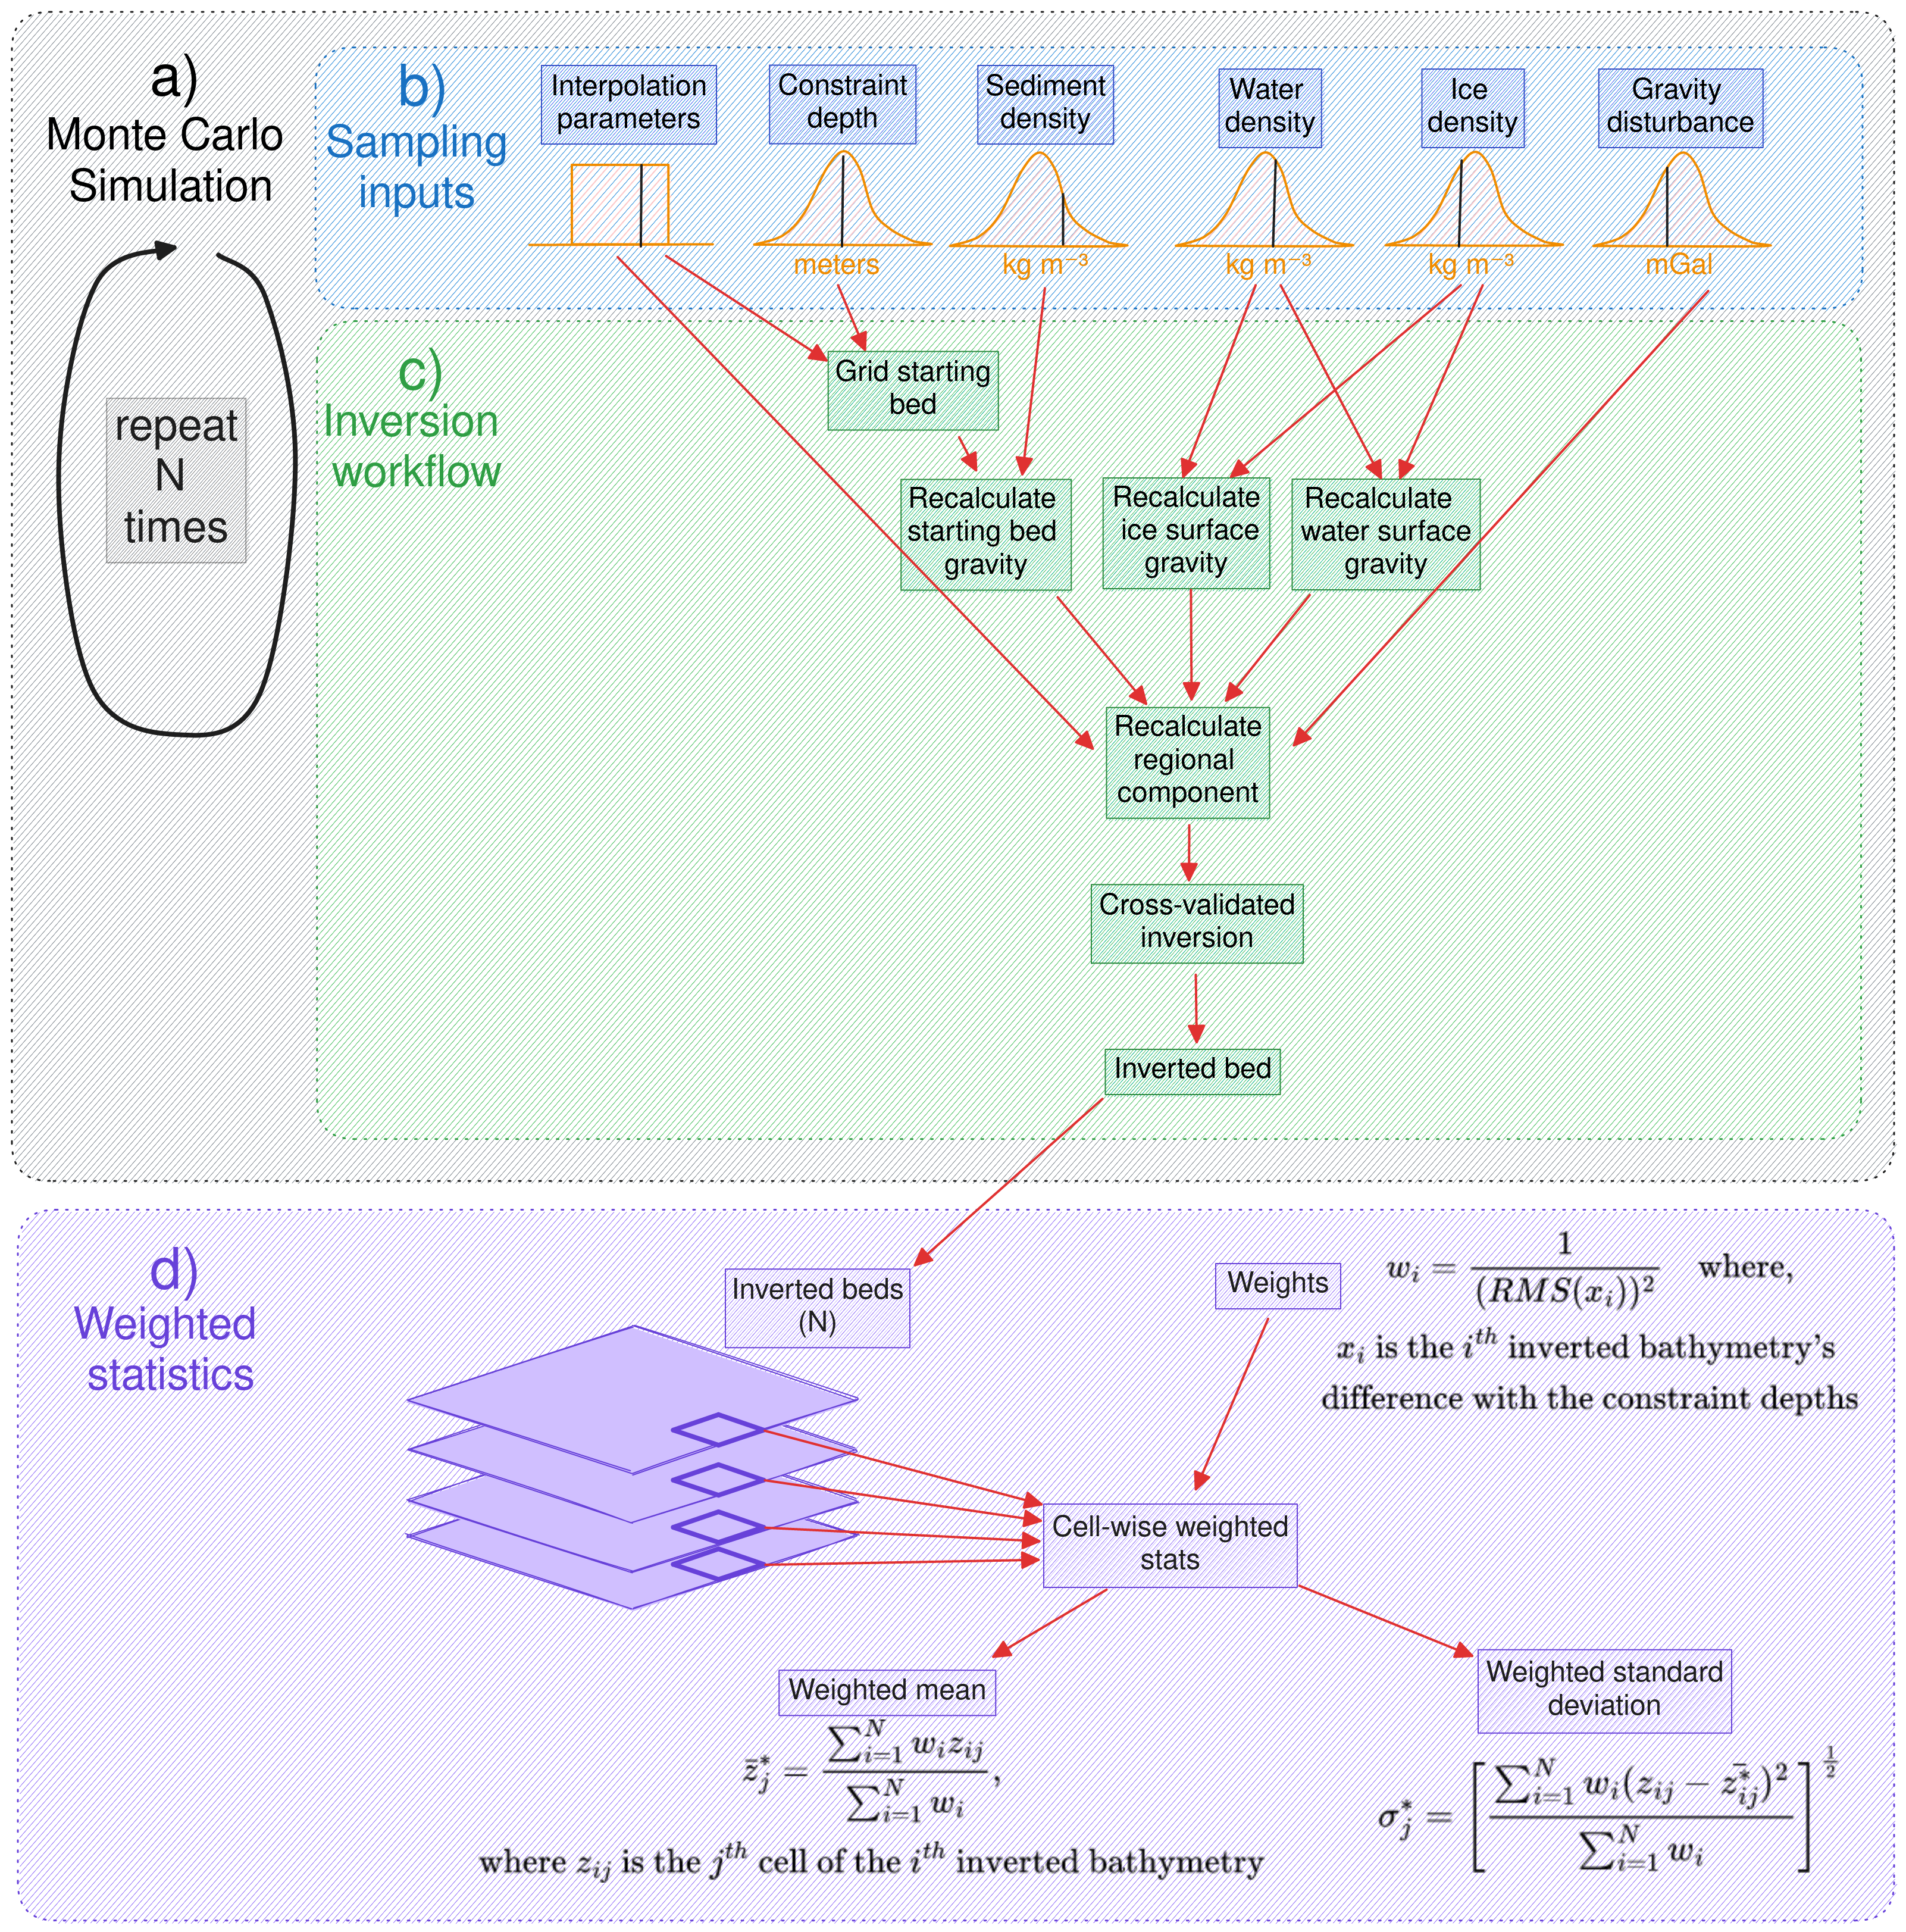
\includegraphics[width=0.99\textwidth]{figures/chp4/Monte_Carlo_workflow.png}
    \caption[Schematic Monte Carlo workflow diagram]{Schematic workflow diagram for the Monte Carlo uncertainty analysis. \textbf{a)} The Monte Carlo simulation, consisting of \textbf{b)} sampling the inputs from their respective distributions, and \textbf{c)} implementing the various components of the workflow, depending on which inputs have been sampled. This process is repeated $N$ times, yielding $N$ inverted bathymetry grids. \textbf{d)} Weighted cell-specific statistics are computed. Each inverted bathymetry grid (large purple boxes) is weighted by the respective inversion's constraint depth RMSE. These weights are used to compute the weighted mean and weighted standard deviation of each grid cell (bold purple square).}
    \label{fig:chp4_Monte_Carlo_workflow}
\end{figure}

The parameters included in the Monte Carlo sampling are: 1) the gravity disturbance data, 2) the constraints point depths, 3) the gridding parameters to create the starting bathymetry, 4) the density of ice, 5) the density of water, 6) the density of sediment, and 7) gridding parameters for the constraint point minimization technique of regional gravity estimation (Figure \ref{fig:chp4_Monte_Carlo_workflow}b). For the full Monte Carlo simulation, with all the above inputs sampled from their respective distributions, the entire inversion workflow needs to be repeated with each of the $N$ parameter sets. This includes 1) creating the starting bathymetry model from the constraint points (Section \ref{chp4_starting_bed_method}), 2) calculating the terrain mass effect to get the topo-free gravity disturbance (Section \ref{chp4_topo_mass_effect}), 3) estimating the regional component of the disturbance and removing it (Section \ref{chp4_regional_separation_method}), and 4) running the damping parameter value cross-validation (Section \ref{ch4_inversion_method}) to obtain the inverted bathymetry (Figure \ref{fig:chp4_Monte_Carlo_workflow}). For the individual Monte Carlo simulations, only portions of this workflow need to be repeated. For example, if only the gravity disturbance is sampled, only the regional field and inversion need to be re-run. The starting bed and topographic mass effect calculated during the baseline inversion are re-used. \\

\begin{figure}[!ht]
  \centering
    \begin{subfigure}[t]{.35\textwidth}
        \centering
        \includegraphics[width=\textwidth]{figures/chp4/random_sampling.png}
        \caption{Random sampling}
    \end{subfigure}
    \begin{subfigure}[t]{.35\textwidth}
        \centering
        \includegraphics[width=\textwidth]{figures/chp4/latin_hypercube_sampling.png}
        \caption{Latin hypercube sampling}
    \end{subfigure}
    \caption[Random vs Latin hypercube sampling]{Comparison of sampling methods for a Monte Carlo simulation of two variables ($X_1$ and $X_2$) with 9 samples drawn from each. \textbf{a)} Random sampling, where values are drawn at random from each variable's distribution, and \textbf{b)} Latin hypercube sampling, where values are drawn from equal-probability intervals. Note the effective coverage of the distributions in \textbf{b} relative to \textbf{a}. The figure is adapted from \citet{kochautomated2017}.}
    \label{fig:chp4_latin_hypercube_sampling}
\end{figure}

Due to the computational demand of a full inversion workflow, the total number of inversions in each Monte Carlo simulation is limited. To ensure the uncertainty distributions of the inputs are adequately sampled with this limited number of possible runs, we have used Latin hypercube sampling where possible \citep{jansenmonte1994}. This sampling technique is well suited for computationally demanding tasks since it ensures proper coverage of the uncertainty distributions of the sampled values, despite a low number of samples \cite{heltonsurvey2006}. To accomplish this, for a Monte Carlo simulation of $N$ runs, the given distributions are split into $N$ intervals of equal probability and one value is chosen from each interval. The $N$ values for each parameter are then randomly paired to get $N$ sets of sampled input parameter values \citep{heltonsurvey2006}. Since the gravity data and constraint points are each sampled on a point-by-point basis, Latin hypercube sampling is unnecessary and random sampling is used. Figure \ref{fig:chp4_latin_hypercube_sampling} shows a $N=9$ comparison of random sampling and Latin hypercube sampling for a two-parameter simulation. \\


\section[Past inversions]{Relation to past bathymetry inversions\sectionmark{Past inversions}} \label{chp4:past_inversions}

The fundamental theory in all bathymetry inversions is based on the fact that the density contrast across the bathymetry surface produces a measurable gravity effect. This phenomenon gives rise to several techniques to convert observed gravity data into bathymetric depths. This by definition is a geophysical inverse problem \citep{oldenburginversion2005}, but the methods chosen to solve it vary from 3D rigorous inversions to iterative 2D forward modelling. Our inversion method follows a classical least-squares approach to solving the inverse problem, while our uncertainty and sensitivity analysis follows a Bayesian approach \citep{asterparameter2018}. Here, we compare our inversion method and workflow to other bathymetry inversions. We attempt to include all past studies related to Antarctica, as well as several from Greenland. We start by comparing our technique for the gravity reduction process, followed by differences in the actual inversion, and finally by differences in our assessment of uncertainty. \\

\subsection{Gravity reduction comparison}

One of the largest differences between our method and past studies is the gravity reduction process. We employ a rigorous terrain mass effect calculation to obtain a topo-free gravity disturbance, often referred to as a Complete Bouguer Anomaly \citep{vajdasecondary2007}. Theoretically, this gravity signal contains only effects due to subsurface density anomalies and inaccuracies in calculating the terrain mass effect. Our method isolates the gravity effect of this inaccuracy since it is due to the deviations between the starting model of bathymetry and the true bathymetry. This is referred to as our residual component of the topo-free gravity disturbance. While most other bathymetry inversion studies achieve a similar residual anomaly, they complete this procedure in a theoretically different way, which may be introducing unnecessary errors. The differences arise from other studies ignoring the reference surface (the ellipsoid) for all calculations after the normal gravity correction.\\

The sign of a gravity disturbance value informs the interpreter as to whether the true Earth has either excess or deficient mass at that location with respect to the normal Earth. Therefore, the absolute level of gravity disturbance data should be retained, even though direct offsets (DC shifts) don't alter the amplitude of the gravity anomalies. For this reason, the reference surface used in the normal gravity calculation (here the ellipsoid) should be continued to be used in all further calculations of topographic masses, including in the forward calculation made during the inversion, as shown in Figure \ref{fig:chp4_discretized_topo_mass_effect} b. Many studies instead have discretized the ice, water, and starting bathymetry surfaces into prism layers which either have arbitrary references or density values not relative to the normal Earth model. This alternative discretization is shown in Figure \ref{fig:chp4_discretized_topo_mass_effect}f-h. For example, the gravity effect of ice, if not just ignored \citep[e.g.,][]{yangfeasibility2020, cochraninversion2012, jordannew2020, millanbathymetry2017}, is typically removed via a "stripping" technique \citep{vajdaglobal2008}, \citep[e.g.,][]{yangbathymetry2021, millanconstraining2020, mutosubglacial2013,greenbaumocean2015}. This stripping involves calculating the forward gravity of prisms with tops defined by the ice surface, bottoms defined by the ice base, and densities defined by the assumed density of ice (Figure \ref{fig:chp4_discretized_topo_mass_effect}f). Additionally, the prisms which comprise the starting bathymetry model for many inversions are bound above by the starting bathymetry, and below by an arbitrary constant depth (Figure \ref{fig:chp4_discretized_topo_mass_effect}h) \citep[e.g.,][]{mutosubglacial2013, tintoross2019}. The forward gravity calculations of this style of discretization can introduce several errors.
\begin{enumerate}
    \item The largest of these errors is an offset in the mean value of the forward gravity relative to the observed gravity. This offset needs to be estimated and removed prior to comparison with the observed data. The DC-shift used to remove the offset is typically estimated by finding a value that minimizes the difference between the observed and predicted data at locations of known bathymetry \citep[e.g.,][]{boghosianresolving2015, cochrandetailed2020, eisermannbathymetry2020, constantinoseafloor2020, mutosubglacial2013, millanbathymetry2017}. This additional step, referred to as "pinning", is unnecessary in our implementation, due to adhering to a rigorous determination of the terrain mass effect. If an incorrect DC shift is applied, the significance of the zero level of the topo-free gravity disturbance is lost. The value of 0 signifies that the simplified model of the Earth (i.e. the starting bathymetry model) is equal to the true Earth density distribution. Shifting this zero-level due to errors in estimating the DC-shift may lead to a vertical offset in the inverted bathymetry, especially if the inversion domain isn't well constrained. The DC-shifted terrain mass effect and the rigorous terrain mass effect for Antarctica are compared in Figure \ref{fig:chp4_antarctic_topo_free_disturbance}d.
    
    \item The forward gravity calculation with this style of discretization results in slightly different amplitude anomalies compared to the true terrain mass effect. This difference is due to the different densities assigned to the prism layer between the two techniques (Figure \ref{fig:chp4_discretized_topo_mass_effect}). While this difference is likely below the range of uncertainties in the gravity error, it is an unnecessary addition of error to the gravity reduction process.
    
    \item The last drawback to using this alternative discretization is an increased gravitational edge effect. As shown in Figure \ref{fig:chp4_discretized_topo_mass_effect}, the average densities and prism heights are larger with this technique. This increases the overall decay of calculated gravity at the edges of the model space, due to the contrast with the void-space beyond the model domain. To account for this, a larger buffer zone is needed, which can significantly increase the computational requirements during forward modelling (see Chapter \ref{ch:3} Section \ref{chp3_edge_effects}).
\end{enumerate}

\subsubsection{Regional separation}
The last step in the gravity reduction process for bathymetry inversion is separating the regional and residual signals, where the residual signal should theoretically be entirely a result of the bathymetry surface. Some techniques commonly used for this are described in Chapter \ref{ch:3} Section \ref{chp3_regional_seperation}. Past bathymetry inversions have used a variety of these techniques, as summarized below.

\begin{enumerate}
    \item Zero or uniform adjustment; For small inversion domains the regional field is sometimes assumed to be minimal. In these scenarios, past studies have either limited the inversion domain to where the regional field is assumed small \citep{cochraninversion2012, boghosianresolving2015}, used a uniform value for the regional component \citep{mutobathymetry2013}, or found a constant density value for the starting model which minimize the gravity misfit \citep{millanvulnerability2018, millanbathymetry2017, anbed2017}.
    
    \item Low-pass filtering; for inversion domains with an expected regional field slightly larger than the above scenario, low-pass filtering of the gravity data can approximate the regional component \citep{eisermannbathymetry2020, hodgsonfuture2019}. 
    
    \item Geologic modelling; To account for the regional field, some studies create geologic models of varying density to estimate the regional field. These models are typically informed from other geophysical data \citep{hodgsonfuture2019, greenbaumocean2015}, \textit{a priori} geologic knowledge \citep{tintoprogressive2011, cochranbathymetric2014, constantinoseafloor2020}, or from an approximated crustal density distribution \citep{tintoross2019, cochrandetailed2020, eisermannbathymetric2021, weigetz2020}.
    
    \item Upwards continuation / high altitude surveys; This technique estimates the long-wavelength regional component by either upward continuing the gravity data to large altitudes, using separate gravity data collect from high-altitude surveys \citep{mutosubglacial2016}, or a combination of both \citep{tintobathymetry2015}
    
    \item Constraint point minimization; the last commonly used technique utilizes the assumption that the desired residual component is near-zero at points of known bathymetry. From this assumption, the regional component at these constraint points is entirely equal to the gravity anomaly value. To estimate the regional field, the gravity values are sampled at the constraint points and interpolated over the region. This technique has been used in several recent inversions where sparse constraint points are available \citep{millanconstraining2020, yangbathymetry2021, yangocean2020, anbathymetry2019, anbathymetry2019a, jordannew2020, vaňkováhigh2023}. While implemented in a different method, this constraint point minimization follows the same concept as several studies which use the constrained locations to derive a spatially variable density model, accounting for the regional field \citep{tintoross2019, eisermannbathymetric2021, weigetz2020}.
\end{enumerate}

Here, we use the constraint point minimization technique for estimating and removing the regional component of the topo-free gravity disturbance.

\subsection{Inversion comparison}

We have developed a conventional non-linear geometric gravity inversion algorithm, as often used in modelling density contrasts, such as sedimentary basins \citep[e.g.,][]{martinssimultaneous2010, santosefficient2015}, or the Moho \citep[e.g.,][]{uiedafast2017, pappamoho2019}. This algorithm is similar in concept to inversions used in other bathymetric studies but differs in its implementation. Past inversion techniques used for bathymetry modelling can be grouped into several categories;
\begin{enumerate}
    \item algorithmic approaches. This method termed the "topographic shift method" \citep{hodgsonfuture2019, jordannew2020}, while not a formal inversion, calculates the equivalent rock thickness from the residual component of gravity, adds this to the starting bathymetry model, and constrains the results by the locations of known bathymetry.
    
    \item 2D profile inversions. Using the method of \citet{talwanirapid1959}, and often implemented within the commercial software Geosoft Oasis Montaj, these inversions retain the 2D nature of the airborne flight lines and invert only along the path of the flight \citep{tintobathymetry2015, cochranbathymetric2014, weigetz2020, boghosianresolving2015, cochrandetailed2020, tintoprogressive2011, constantinocook2023}.
    
    \item 3D frequency-based inversions. This category of inversion uses a Fourier transformation to calculate the forward gravity effect of a continuous topographic surface, forgoing the need to discretize the topography into vertical prisms \citep{parkerrapid1972, oldenburginversion1974}. This Fourier transform is then iteratively modified to minimize the misfit to the observed gravity. This method, particularly its implementation within the commercial software Geosoft Oasis Montaj, is frequently used for bathymetry inversions \citep{anbathymetry2019a, anbathymetry2019, anbed2017, greenbaumocean2015, millanconstraining2020, eisermannbathymetry2020, cochraninversion2012, millanvulnerability2018, millanbathymetry2017, studingerestimating2004, eisermannbathymetric2021}.
    
    \item Simulated Annealing. This global optimization technique \citep{kirkpatrickoptimization1983} performs many forward calculations of possible bathymetry surfaces and slowly converges on a model which minimizes the misfit with the observations. This method, similar to our Monte Carlo uncertainty analysis, has the benefit of providing an uncertainty estimate of the resulting bathymetry based on the uncertainty in the inversion inputs. This has been used in several bathymetric inversions \citep{royinversion2005, mutosubglacial2013, mutosubglacial2016, yangocean2020, yangbathymetry2021, yangseafloor2018, filinanew2008}

    \item Regularized least-squares inversions. This style of inversion is the conventional approach to solving non-unique inverse problems \citep{asterparameter2018}. While this method is commonly used for other geometric gravity inversions (e.g., Moho and basement), to our knowledge it is only applied to bathymetry inversions here, and in \citet{vaňkováhigh2023}.
\end{enumerate}

\subsection{Uncertainty comparison}

Here we compare our uncertainty analysis to those from other bathymetry-gravity inversion studies. Most of these past studies provide an estimation of uncertainty, but only a few provide spatially variable uncertainties \citep[e.g.,][]{anbathymetry2019, mutosubglacial2016}. Typically, these inversion uncertainties are assumed to result from three sources.

\begin{enumerate}
    \item Uncertainty in the gravity data. The uncertainties resulting from the gravity data uncertainty are typically estimated using a Bouguer slab approximation, with an assumed density of the contrast between rock and water ($\sim$~1600~kg~m\textsuperscript{-3}), and a gravity uncertainty approximated from the RMS crossover values of the airborne gravity survey \citep[e.g.,][]{tintoross2019, constantinoseafloor2020, boghosianresolving2015}. Alternatively, a simple conversion factor has been proposed of 100~m of inversion uncertainty per 5~mGal of gravity uncertainty \citep{anbathymetry2019, anbathymetry2019a}.

    \item Assumptions of the geologic structure. The uncertainty resulting from assumptions of the geologic structure is typically simplified as uncertainties in the choice of the constant density contrast between sediment and seawater. This uncertainty is sometimes approximated as a ratio of change in density to change in inverted relief as a percentage \citep[e.g., $\sim$3\% relief for 50~kg~m\textsuperscript{-3}][]{tintoross2019} or by altering the density and comparing the results \citep{boghosianresolving2015}.

    \item Uncertainties in the past measurements of bathymetry (constraints). Lastly, constraint point measurement uncertainties are typically assumed to result in a 1:1 uncertainty in the inverted bathymetry \citep[e.g.,][]{tintoross2019, boghosianresolving2015}.
\end{enumerate}

Our uncertainty analysis, through Monte Carlo simulation, provides robust spatial uncertainty estimates for each of these three sources of uncertainty. Similar to the above methods, Monte Carlo simulation only addresses uncertainties related to the uncertainty of the inputs to the inversion.

\section{Results}

Here we apply the above-described methods to recover a higher resolution bathymetry beneath Antarctica's Ross Ice Shelf. First, we show the results from an individual workflow, as depicted in Figure \ref{fig:chp4_workflow}. This includes the starting bathymetry model, the topo-free gravity disturbance calculations, and the resulting inverted bathymetry. Next, we present the Monte Carlo simulation results, where this entire workflow is repeated many times with varying values of input data and parameters.\\

\subsection{Starting bathymetry}

Existing options for a starting bathymetry model for the sub-Ross Ice Shelf include Bedmap2 \citep{fretwellbedmap22013} or BedMachine v3 \citep{morlighemdeep2020, morlighemmeasures2022}. BedMachine v3 for the Ross Ice Shelf contains the gravity-inverted bathymetry results from \citet{tintoross2019}. To avoid over-interpretation of the gravity data (starting an inversion with the results of a separate inversion) we opted to not use BedMachine for the starting model. Bedmap2 bed elevations for the Ross Ice Shelf were created through the interpolation of the point constraints \citep{fretwellbedmap22013}. These point constraints within the ice shelf (Figure \ref{fig:chp4_inversion_inputs}b) were compiled from several surveys, including the early traverses of the 1950s and 60s \citep{craryglaciological1962,  craryoversnow1959,craryoversnow1962}\footnote{These surveys included the Ross Ice Shelf Traverse (1957-1958), the Little America Station Byrd Trail Traverse (1958), the Victoria Land Traverse (1958-1959), and the Discovery Deep Traverse (1960), see \citet{bennettgravity1964} for the data and descriptions.}, and the Ross Ice Shelf Geophysical and Glaciological Survey \citep[RIGGS, 1973-1974][]{bentleyross1984} ($N=223$). However, the gridding algorithm used (ArcGIS Topogrid), while producing smooth results for the Ross Ice Shelf, didn't strictly adhere to the constraint point depths. This can be seen through the comparison of constraint point depths and Bedmap2 grid values at the same location (Figure \ref{fig:chp4_inversion_inputs}b). The RMS difference between the constraint depths and the grid depths within the ice shelf is 138~m. The largest differences are concentrated along the Transantarctic Mountain Front, where Bedmap2 grid values are much shallower than the constraint points. Due to this over-smoothing of the constraints, we have opted to create our own starting bathymetry model.\\

Our starting model was created from the combination of various seismic survey constraint points on the ice shelf, and bed data from BedMachine v3 \citep{morlighemdeep2020, morlighemmeasures2022} outside of the ice shelf. To create this, the BedMachine v3 bed elevations, relative to the WGS-84 ellipsoid, were masked within the Ross Ice Shelf, based on the MEaSUREs v2 Ross Ice Shelf boundary \citep{mouginotmeasures2017, rignoticeshelf2013}. These data were converted from gridded data into point data and merged with the various bathymetry data within the ice shelf. A continuous grid of bathymetry depths at a 5~km cell size was then interpolated from the combined data inside and outside the shelf. The interpolation can be accomplished with two gridding methods, bi-harmonic splines \citep{sandwellbiharmonic1987}, and minimum curvature \citep{smithgridding1990}. While the bi-harmonic spline method appears to have several advantages over minimum curvature (Chapter \ref{ch:3} Section \ref{chp3_gridding_comparison}), such as the ability to apply weights to the data, interpolating the above Ross Ice Shelf data resulted in significant unconstrained minima and maxima. Initial inversion results showed these erroneous features carry through to the final inverted bathymetry. Due to this, we have opted to interpolate the data to create the starting bathymetry model using tensioned minimum curvature. This method resulted in less extreme un-constrained minima and maxima.\\

% Both of these methods contain a parameter that must be chosen. For the minimum curvature method, this parameter is the tension factor (Section \ref{chp3_gridding_comparison}), which ranges from 0 to 1. For bi-harmonic splines, the parameter is a damping value applied to the interpolation. This damping is necessary in order to for the interpolation to account for the differing uncertainties of each constraint point \citep{uiedaverde2018}. This avoids an interpolation bias to highly uncertain data. Points outside of the ice shelf were assigned a constant uncertainty of 10 m, reflecting the relatively low uncertainty in determining bed elevation over grounded ice, or open ocean. Points within the ice shelf were assigned uncertainties of 5\% of their depth from the ice surface, equating to a mean uncertainty of 34 m. \\

\begin{figure}[!ht]
    \centering
    \includegraphics[width=0.98\textwidth]{figures/chp4/starting_bed_comparison.png}
    \caption[Ross Ice Shelf starting bathymetry]{Starting bathymetry models from the interpolation of constraint points within the ice shelf and BedMachine v3 gridded data outside of the shelf \citep{morlighemdeep2020, morlighemmeasures2022}. The ice shelf border, from \citet{mouginotmeasures2017}, is shown as the solid black line, representing the grounding line and the calving front. \textbf{a-f)} Bathymetry models resulting from 6 varying tension factor values of minimum curvature interpolation. Contours shown at 400~m intervals. \textbf{g)} The cell-specific weighted standard deviation of the six models (\textbf{a-f}). \textbf{h)} The cell-specific weighted mean bed elevation from the six models. \textbf{i)} The difference between Bedmap2 bathymetry and the mean model (\textbf{h}). The RMS difference is 95~m. Blues show where the mean model is shallower than Bedmap2, while reds show where the mean model is deeper. Root mean square error (RMSE) values in the plot titles are between the constraint point depths and the values at those points on the interpolated grids.}
    \label{fig:chp4_starting_bed_comparison}
\end{figure}

To test the importance of the tension value used in the minimum curvature gridding, we performed 6 interpolations, with tension values of 0, 0.2, 0.4, 0.6, 0.8, and 1 (Figure \ref{fig:chp4_starting_bed_comparison}a-f). From these six resulting bathymetry models, we calculated the standard deviation (Figure \ref{fig:chp4_starting_bed_comparison}g) and the cell-specific mean (Figure \ref{fig:chp4_starting_bed_comparison}h). These statistics were weighted, in the same method described in Figure \ref{fig:chp4_Monte_Carlo_workflow}d. The weight value used for each grid was the inverse square of the RMS difference between the constraint point depth values and the resulting grid values at the same points. These RMS values are shown in the figure titles of Figure \ref{fig:chp4_starting_bed_comparison}a-f. This weighted mean starting model is compared to Bedmap2 bathymetry (Figure \ref{fig:chp4_starting_bed_comparison}i). Note that while low tension factors result in models that closely match the constraints, they also produce local maxima and minima away from the data, which is not ideal since these features can be seen to carry through the inversion to the final bathymetry, as discussed later. Alternatively, higher tension values produce models that don't match the constraints as well (higher RMS values), but they don't have as many erroneous features. For this reason, we use the cell-specific mean of the six models as our starting bathymetry (Figure \ref{fig:chp4_starting_bed_comparison}h). This model has an RMS difference from BedMap2 within the ice shelf of 95~m.\\

\begin{figure}[!ht]
    \centering
    \includegraphics[width=0.5\textwidth]{figures/chp4/RIS_weighting_grid.png}
    \caption[Ross Ice Shelf weighting grid]{Weighting grid used in the Ross Ice Shelf bathymetry inversion. Grid colours show both the distance between each grid cell and the nearest constraint point and the weight values (0 - 1) from the normalization of these distances. Constraint points are defined as either direct measurements of bathymetry within the ice shelf (black crosses), or any grid cell outside of the ice shelf (small black dots). The ice shelf border, from \citet{mouginotmeasures2017} is shown as the solid black line, representing the grounding line or the calving front.}
    \label{fig:chp4_RIS_weighting_grid}
\end{figure}

From these constraint points used to create the starting bathymetry, a weighting grid was created (Figure \ref{fig:chp4_RIS_weighting_grid}). This grid was calculated from the distance between each grid cell and the nearest constraint point. This minimum constraint distance (top annotations of Figure \ref{fig:chp4_RIS_weighting_grid} colourbar) was then normalized between 0 and 1 to create the weighting grid (bottom annotations of Figure \ref{fig:chp4_RIS_weighting_grid} colourbar). As all grid cells outside of the ice shelf border are considered constraint points non-zero weights and  minimum constraint distances are confined to within the ice shelf border. The colourbar histogram shows a mean minimum constraint distance within the ice shelf of approximately 20~km, and an upper limit of approximately 60~km. Within the shelf, there are 223 constraint points. Over an area of $\sim$480,000~km\textsuperscript{2} \citep{mouginotmeasures2017}, this equates to a constraint density of $\sim$1 constraint per $46\times46$~km (2154~km\textsuperscript{2}).\\


\subsection{Gravity processing results} \label{chp4_gravity_processing_results}

We use airborne gravity data from the Ross Ocean and ice Shelf Environment, and Tectonic setting Through Aerogeophysical surveys and modelling project (ROSETTA-Ice). This project was created with the goal of investigating the interactions between ice, ocean, and earth of Antarctica's Ross Ice Shelf \citep{tintoross2019}. The survey consisted of 3 field seasons (2015-2017) of airborne geophysical surveying with a survey design consisting of E-W flight lines, at a nominal spacing of 10~km, and N-S tie lines with a nominal spacing of 55~km (Figure \ref{fig:chp4_inversion_inputs}a). Flights were flown at an average of 750~m above the ice surface and a speed of 180~knots (93~ms\textsuperscript{-1}), The survey was designed to maximize the overlap between the flight lines and the past bathymetry constraints across the ice shelf from the RIGGS seismic surveys \citep{bentleyross1984}. The data collection and initial processing were performed by \citet{tintoross2019} and are briefly summarized here. The gravity data were collected with a combination of a LaCoste and Romberg gravimeter upgraded with a ZLS UltraSys control system, an iMAR inertial measurement unit, and a DgS gravimeter. The ZLS data were tied to an absolute gravity reference station at McMurdo Station. Poor-quality data from the ZLS were replaced with the iMAR or DgS values. The accelerations of the aircraft were calculated from GPS data and removed from the gravity signal. The E\"{o}tv\"{o}s correction was applied, to account for measuring gravity on a moving platform \citep{harlaneotvos1968}. At each observation point, the effects of the normal earth were calculated and removed, giving the gravity disturbance values (See Section \ref{ch4 normal gravity}). Levelling was then performed using the cross-over values between E-W flight lines and N-S tie lines.\\

\begin{figure}[!ht]
    \centering
    \includegraphics[width=0.6\textwidth]{figures/chp4/ROSETTA_levelling_convergence.png}
    \caption[Re-levelling of the ROSETTA-Ice gravity data]{Re-levelling of the ROSETTA-Ice gravity data. First, flight lines were individually upward continued, then cross-over point misties were found. These were used in 0\textsuperscript{th}, 1\textsuperscript{st}, and 2\textsuperscript{nd} order iterative levelling, alternative between levelling flight lines to tie lines and vice versa at each iteration. The RMS cross-over errors at each iteration are shown. The major steps show the 0\textsuperscript{th}, 1\textsuperscript{st}, and 2\textsuperscript{nd} order stages of levelling.}
    \label{fig:chp4_levelling}
\end{figure}

Since this bathymetry inversion is strongly influenced by noise in the gravity data, as demonstrated in Chapter \ref{ch:3} Section \ref{chp3_effect_of_gravity_noise}, we have performed additional processing to the published ROSETTA-Ice dataset. Erroneous sections of flight line data were manually removed, and the dataset was re-levelled. The levelling procedure utilizes the gravity difference between E-W and N-S flight lines at cross-over points. While the flight paths intersect in 2-D space, their altitudes typically differ, meaning there is no true cross-over point in 3-D space. To account for this, the flight lines are individually upward continued to a constant elevation of 1~km (ellipsoidal height). The mean elevation of the cleaned data was $\sim$790~m, and 1~km was greater than 96\% of the data. This limited the amount of downward continuation while retaining a spatial resolution close to the original data. This continuation was calculated using the equivalent source technique \citep[see Section \ref{chp3:eq source resampled}][]{dampneyequivalent1969, solergradientboosted2021}. Since the cross-over points are now true 3-D intersections, the difference between E-W and N-S lines at these points (mis-ties) can be used to re-level the dataset. Here, we alternate between levelling the E-W lines to the N-S lines, and vice versa. We start with a 0\textsuperscript{th} order levelling, where only DC shifts are applied. Followed by a 1\textsuperscript{st} and 2\textsuperscript{nd} order levelling, where 1 and 2-degree polynomials, respectively, are fit to the mis-ties, and used to level the lines. The results of this levelling procedure are shown in Figure \ref{fig:chp4_levelling}. For each order of levelling several iterations are performed. The step-wise convergence of the RMS mis-tie values shows the 0\textsuperscript{th}, 1\textsuperscript{st}, and 2\textsuperscript{nd} order levelling stages. The re-levelling procedure brought the RMS mis-tie from $\sim$4.8~mGal to $\sim$3.2~mGal. \\

Finally, this re-levelled gravity disturbance line data were gridded onto a regular grid at 2.5~km spacing, using equivalent sources. Since the inversion only affects the bathymetry within the ice shelf border, as implemented with the weighting grid (Figure \ref{fig:chp4_RIS_weighting_grid}), the interpolated gravity grid is masked beyond 10~km outside of the ice shelf border (Figure \ref{fig:chp4_levelling}b). This 2.5~km gridded data ($N=85,914$) consists of both the \textit{testing} ($N=64,435$) and \textit{training} ($N=21,479$) sets used in the cross-validation. With the grid configuration shown in Chapter \ref{ch:3} Figure \ref{fig:chp3_CV_grid_spacing}, the \textit{training} data used in the actual inversion are on a regular 5~km grid. \\

\subsection{Gravity reduction results}

The terrain mass effect was calculated at each of the gridded gravity data points. For this calculation, the three layers of prisms shown in Figure \ref{fig:chp4_discretized_topo_mass_effect}c-e were created from BedMachine v3 \citep{morlighemdeep2020, morlighemmeasures2022} ice surface and water surface data and the mean starting bathymetry from Figure \ref{fig:chp4_starting_bed_comparison}h. All data are referenced to the WGS-84 ellipsoid. The ice surface elevations used from BedMachine v3 are in ice equivalent, meaning they have had a firn depth correction applied, making for a slightly lower surface elevation to account for spatially variable firn thickness \citep{morlighemdeep2020}. An ice equivalent surface is suitable for calculating the terrain mass effect since it gives the estimated thickness of the ice shelf with a density of ice, instead of the true ice shelf thickness, with a layer of low-density firn above. Comparing the forward gravity calculated from the true geometry of ice shelf thickness, the ice equivalent thickness, and a 2-layer model with firn and ice, show minimal differences, and thus we use the ice equivalent thickness in the terrain mass effect. The densities used in the terrain mass effect calculations were 1~kg~m\textsuperscript{-3} for air, 915~kg~m\textsuperscript{-3} for ice, 1024~kg~m\textsuperscript{-3} for seawater \citep{griggsantarctic2011}, and 2300~kg~m\textsuperscript{-3} for seafloor. Since we use a single value for the density of the seafloor, it should represent the expected average density of the seafloor over the entire region. Chapter \ref{ch:2} showed a continuous drape of sediment over the seafloor. We chose 2300 kg m\textsuperscript{-3} to be in the middle between unconsolidated sediment ($\sim1900$~kg m\textsuperscript{-3}) and low-density crystalline rock ($\sim2700$~kg m\textsuperscript{-3}) \citep{schöndensity2015}. The inversion domain was 1 million km\textsuperscript{2} (1000~km~$\times$~1000~km). To avoid gravitational edge effects in the forward calculations, the prism layers were extended in all directions by a 40~km buffer zone, resulting in 120,000 prisms. The resulting terrain mass effect was subtracted from the gravity disturbance to get the topo-free gravity disturbance. These data are shown in Figure \ref{fig:chp4_RIS_terrain_regional_residual}.\\

\begin{figure}[!ht]
  \centering
    \begin{subfigure}[t]{.99\textwidth}
        \centering
        \includegraphics[width=\textwidth]{figures/chp4/RIS_terrain_regional.png}
    \end{subfigure}
    \begin{subfigure}[t]{.8\textwidth}
        \addtocounter{subfigure}{4}
        \centering
        \includegraphics[width=\textwidth]{figures/chp4/RIS_terrain_regional_profile.png}
        \caption{}
    \end{subfigure}
  \caption[Gravity reduction results for the Ross Ice Shelf]{Gravity reduction results for the Ross Ice Shelf. \textbf{a)} Gravity disturbance, \textbf{b)} topo-free gravity disturbance, after the removal of the terrain mass effect, \textbf{c)} regional component of the topo-free disturbance, estimated with constraint point minimization, and \textbf{d)} residual component of the topo-free disturbance, as the difference between \textbf{b} and \textbf{c}. Background imagery is from MODIS-MOA \citep{scambosmodisbased2007} and grounding line and coastlines are from \citep{morlighemmeasures2022}. Constraint points within the ice shelf are shown as dots. \textbf{e)} Profile from A to A', location shown in \textbf{d}. \textbf{Upper panel} shows cross-section, with ice surface and ice base from BedMachine v3 \citep{morlighemdeep2020, morlighemmeasures2022}. Brown layer shows the mean starting bed model with bounding uncertainty (light brown lines) from the standard deviation of the various starting bed models in Figure \ref{fig:chp4_starting_bed_comparison}. The colour of ice surface shows the distance to the nearest constraint point. \textbf{Lower panel} shows data from \textbf{a-d} along the profile.}
    \label{fig:chp4_RIS_terrain_regional_residual}
\end{figure}

% \begin{figure}[!ht]
%   \centering
%     \begin{subfigure}[t]{.95\textwidth}
%         \centering
%         \includegraphics[width=\textwidth]{figures/chp4/RIS_terrain_effects.png}
%     \end{subfigure}
%     \begin{subfigure}[t]{.8\textwidth}
%         \addtocounter{subfigure}{3}
%         \centering
%         \includegraphics[width=\textwidth]{figures/chp4/RIS_terrain_effects_profile.png}
%         \caption{}
%     \end{subfigure}
%   \caption{Terrain mass effect correction. \textbf{a)} Forward calculated terrain mass effect from of BedMachine v3 ice surface, water surface, and the mean starting bed model from Figure \ref{fig:chp4_starting_bed_comparison}h, as discretized accorded to Figure \ref{fig:chp4_discretized_topo_mass_effect}. \textbf{b)} Levelled, upward continued, and gridded gravity disturbance data. \textbf{c)} Topo-free gravity disturbance data from the difference between \textbf{a} and \textbf{b}. Background imagery is from MODIS-MOA \citep{scambosmodisbased2007} and grounding line and coastlines are from \citep{morlighemmeasures2022}. Constraint points within the ice shelf are shown as dots. \textbf{d)} Profile from A to A'. \textbf{Upper panel} Earth layer cross-section, with ice surface and ice base from BedMachine v3 \citep{morlighemdeep2020, morlighemmeasures2022}. Brown layer shows the mean starting bed model with bounding uncertainty (light brown lines) from the standard deviation of the various starting bed models in Figure \ref{fig:chp4_starting_bed_comparison}. Purple points along the ice surface show locations within 5 km of a constraint point or grounded ice. \textbf{Lower panel} shows data from \textbf{a-c} along the profile.}
%     \label{fig:chp4_RIS_terrain_effects}
% \end{figure}

The topo-free gravity disturbance was subsequently separated into the regional and residual components. This was accomplished with constraint point minimization (Chapter \ref{ch:3} Section \ref{chp3_regional_seperation}). While the synthetic data of the past chapter showed a clear benefit of using a bi-harmonic spline interpolation over a minimum curvature interpolation, we use minimum curvature here. As with the interpolation for the starting bathymetry model, bi-harmonic spline interpolation led to excessive unconstrained maximum or minima. The resulting regional and residual components are shown in Figure \ref{fig:chp4_RIS_terrain_regional_residual}. \\

% \begin{figure}[!ht]
%   \centering
%     \begin{subfigure}[t]{.95\textwidth}
%         \centering
%         \includegraphics[width=\textwidth]{figures/chp4/RIS_regional_residual.png}
%     \end{subfigure}
%     \begin{subfigure}[t]{.8\textwidth}
%         \addtocounter{subfigure}{3}
%         \centering
%         \includegraphics[width=\textwidth]{figures/chp4/RIS_regional_residual_profile.png}
%         \caption{}
%     \end{subfigure}
%   \caption{Regional gravity separation results. \textbf{a)} Topo-free gravity disturbance, separated into regional (\textbf{b}) and residual (\textbf{c}) components. Background imagery is from MODIS-MOA \citep{scambosmodisbased2007} and grounding line and coastlines are from \citep{morlighemmeasures2022}. Constraint points within the ice shelf are shown as dots. \textbf{d)} Profile from A to A'. \textbf{Upper panel} Earth layer cross-section, with ice surface and ice base from BedMachine v3 \citep{morlighemdeep2020, morlighemmeasures2022}. Brown layer shows the mean starting bed model with bounding uncertainty (light brown lines) from the standard deviation of the various starting bed models in Figure \ref{fig:chp4_starting_bed_comparison}. Purple points along the ice surface show locations within 5 km of a constraint point or grounded ice. \textbf{Lower panel} shows data from \textbf{a-c} along the profile.}
%     \label{fig:chp4_RIS_regional_residual}
% \end{figure}

\subsection{Inversion results}

With the residual component of the topo-free gravity disturbance as the inversion input (Figure \ref{fig:chp4_RIS_terrain_regional_residual}d), we ran 10 inversions with varying levels of damping. Each inversion used a density of 1024~kg~m\textsuperscript{-3} for ocean water and 2300~kg~m\textsuperscript{-3} for the density of the seafloor. For each value of the damping parameter, the cross-validation score was calculated by forward modelling the gravity effect of the resulting bathymetry model onto the locations of the testing gravity data. The RMS difference between the residual component of the topo-free gravity disturbance and the forward-modelled results at these testing points gave the score. These scores are shown in Figure \ref{fig:chp4_RIS_inversion_results}a. The lowest score was achieved with a damping value of 10\textsuperscript{-2}. \\

This inversion took 8 iterations and 135 seconds\footnote{See Appendix \ref{chp1_open_source} for a description of the hardware used.} and converged due to a lack of change in the $\ell^2$-norm between subsequent iterations (Figure \ref{fig:chp4_RIS_inversion_results}b). The RMS of the residual gravity started at 6.1~mGal prior to the inversion and was reduced to 4.0~mGal (Fig \ref{fig:chp4_RIS_inversion_results}b). \\

\begin{figure}[!ht]
  \centering
    \begin{subfigure}[t]{.4\textwidth}
        \centering
        \includegraphics[width=\textwidth]{figures/chp4/RIS_damping_CV.png}
        \caption{}
    \end{subfigure}
    \begin{subfigure}[t]{.4\textwidth}
        \centering
        \includegraphics[width=\textwidth]{figures/chp4/RIS_convergence.png}
        \caption{}
    \end{subfigure}
    \begin{subfigure}[t]{.95\textwidth}
        \centering
        \includegraphics[width=\textwidth]{figures/chp4/RIS_inversion_results.png}
        % \caption{}
    \end{subfigure}
    \begin{subfigure}[t]{.8\textwidth}
        \addtocounter{subfigure}{3}
        \centering
        \includegraphics[width=\textwidth]{figures/chp4/RIS_inversion_results_profile.png}
        \caption{}
    \end{subfigure}
  \caption[Ross Ice Shelf singular bathymetry inversion results]{Ross Ice Shelf singular bathymetry inversion results. \textbf{a)} Damping parameter cross-validation with the lowest score shown in red. \textbf{b)} Convergence curve and cumulative inversion time for the optimal inversion. Blue line (left y-axis) shows consecutive iteration's RMS residual component of the topo-free gravity disturbance. Green line (right y-axis) shows cumulative time to run the inversion. \textbf{c)} Inverted bathymetry, \textbf{d)} water column thickness between the inverted bathymetry and Bedmachine v3 icebase \citep{morlighemdeep2020, morlighemmeasures2022}, \textbf{e)} final residual component of the topo-free gravity disturbance. \textbf{f)} \textbf{Profile A to A'}. \textbf{Upper panel} shows ice surface and icebase from BedMachine v3, both the starting bathymetry (dark brown) and the inverted bathymetry (light brown). The colour of the ice surface shows the distance to the nearest constraint point. \textbf{Lower panel} shows the initial residual gravity used as input to the inversion (blue line, left y-axis), and the total correction (red line, right y-axis) applied to the starting bathymetry surface during the inversion to get the inverted bathymetry.}
    \label{fig:chp4_RIS_inversion_results}
\end{figure}

The inverted bathymetry model for the sub-Ross Ice Shelf, at a 5~km resolution, is shown in Figure \ref{fig:chp4_RIS_inversion_results}c. Note that this is just the result of a single inversion. Our final inverted bathymetry model is achieved through the Monte Carlo simulation, as described below. The RMS difference between the inversion results and the starting model at the constraints is 16 m. The thickness of the water column, defined as the difference between BedMachine v3 ice base and the inverted bathymetry, is shown in Figure \ref{fig:chp4_RIS_inversion_results}d. \\

\subsection{Uncertainty}

We used a series of Monte Carlo simulations (Figure \ref{fig:chp4_Monte_Carlo_workflow}) to assess both the spatial uncertainty of the resulting inverted bathymetry and the importance of the various components and parameters of the inversion. By varying the inputs of the inversion within their ranges of uncertainties, we can gather a range of the possible bathymetry results, which when compared shows where the inversion results are more or less certain. The inputs and their respective uncertainty distributions included in the sampling are:
\begin{enumerate}
    \item 
    Gravity disturbance data; sampled from a normal distribution with a mean of the data point, and a standard deviation of the RMS mis-tie of the line data after levelling (3.3~mGal).
    \item 
    Constraint point depths; sampled from a normal distribution with a mean of the measured depth, and a standard deviation of 10~m for points outside of the ice shelf, and 5\% of depth from the ice surface for points within the ice shelf (mean of 36~m).
    \item 
    The density of ice, water, and sediment; all sampled from normal distributions with means of 915~kg~m\textsuperscript{-3}, 1024~kg~m\textsuperscript{-3}, and 2300~kg~m\textsuperscript{-3} respectively, and standard deviations of 5~kg~m\textsuperscript{-3}, 5~kg~m\textsuperscript{-3}, and 400~kg~m\textsuperscript{-3}. The small standard deviations of ice and water compared to sediment reflects the relative certainty of the value and spatial heterogeneity of the density of ice and water, compared to those of the material comprising the sea floor. For the Ross Ice Shelf, the entire region is likely to be draped is at least 10's of meters of sediment \citep[Chapter \ref{ch:2},][]{tankersleybasement2022}. With a mean of 2300~kg~m\textsuperscript{-3} and a standard deviation of 400~kg~m\textsuperscript{-3}, these values span the range from unconsolidated sediment to low-density crystalline rock \citep{schöndensity2015}. 
    \item 
    The tension factor used in minimum curvature gridding for interpolating both the starting bathymetry model and the regional component of gravity. The tension factor values were sampled from a uniform distribution between 0 and 1. 
\end{enumerate}


\begin{figure}[!ht]
  \centering
    \begin{subfigure}[t]{.98\textwidth}
        % \centering
        \hspace*{-1.5cm} %
        \includegraphics[width=\textwidth]{figures/chp4/RIS_LHC_covariance.png}
        \caption{}
    \end{subfigure}
    \begin{subfigure}[t]{.9\textwidth}
        \centering
        \includegraphics[width=\textwidth]{figures/chp4/RIS_LHC_distributions.png}
        \caption{}
    \end{subfigure}
  \caption[Latin hypercube sampling distributions and correlations]{Latin hypercube sampling results for the 10 inversions of the full Monte Carlo simulation. \textbf{a)} Correlations between each pair of the 5 sampled input parameters. \textbf{b)} Resulting distributions of the 10 sampled values of each parameter. Blue line shows kernel density estimates fit to each set of sampled values, which are shown as orange ticks.}
    \label{fig:chp4_RIS_sampling_results}
\end{figure}

Figure \ref{fig:chp4_RIS_sampling_results} shows the results of the Latin hypercube sampling of the 5 input variables (not including the gravity and constraints data). The correlations between each set of variables show that pairwise correlation was minimal. This is ideal since these inputs are unrelated, and therefore their sampled values should be uncorrelated \citep{heltonsurvey2006}. This also shows that with only 10 samplings, the Latin hypercube sampling was able to provide adequate spatial coverage of the individual distributions (\ref{fig:chp4_RIS_sampling_results}b) as well as all the pairwise distributions combinations (\ref{fig:chp4_RIS_sampling_results}a).

\begin{figure}[!ht]
    \centering
    \includegraphics[width=.99\textwidth]{figures/chp4/RIS_MC_bed_and_uncert.png}
    \caption[Ross Ice Shelf inverted bathymetry and uncertainty]{Final bathymetry depths and uncertainties from the full Monte Carlo simulation, merged with 500m resolution elevation and uncertainty data outside of the shelf from BedMachine v3 \citep{morlighemdeep2020, morlighemmeasures2022}. \textbf{a)} Final inverted bathymetry model, calculated as the weighted mean of the full Monte Carlo simulation. Shown with 300~m contours. \textbf{b)} Uncertainty estimation of the inverted bathymetry from the cell-specific weighted standard deviation of the inverted bathymetry results from the full Monte Carlo simulation. Shown with 100~m contours. Constraints within the ice shelf are shown as dots in \textbf{a}. Grounding line and coastline are shown in black \citep{morlighemmeasures2022}. Background imagery is from \citet{scambosmodisbased2007}. Cyan lines show Discovery Deep and Kamb Ice Stream seismic surveys.}
    \label{fig:chp4_RIS_MC_results}
\end{figure}

Each simulation consisted of 10 runs. We performed a \textit{full} simulation, where each of the above inputs were sampled (Figure \ref{fig:chp4_RIS_MC_results}). We performed five additional simulations (Figure \ref{fig:chp4_RIS_MC_sensitivity}) where 1) only the gravity data were sampled, 2) only the constraint point depths were sampled, 3) only the density values of ice, water, and sediment were sampled, 4) only the tension factor for interpolating the starting bathymetry model was sampled, and finally 5) only the tension factor for interpolating the regional component of gravity was sampled. Each simulation results in a series of inverted bathymetries. Finding the cell-specific weighted standard deviation of the bathymetry depths for each of these simulations gives an estimation of the uncertainty resulting from the associated parameter. The cell-specific statistics of these simulations were low-pass filtered to remove high-frequency noise induced by the random sampling. For the full simulation (Figure \ref{fig:chp4_RIS_MC_results}b) the weighted mean of the resulting bathymetries gives the final inverted bathymetry results of this study (Figure \ref{fig:chp4_RIS_MC_results}a). Note that this final bathymetry model resulting from the Monte Carlo simulation is similar, but distinct from the inverted bathymetry resulting from a single inversion without the Monte Carlo simulation, shown in Figure \ref{fig:chp4_RIS_inversion_results}c. \\

\begin{figure}[!ht]
    \centering
    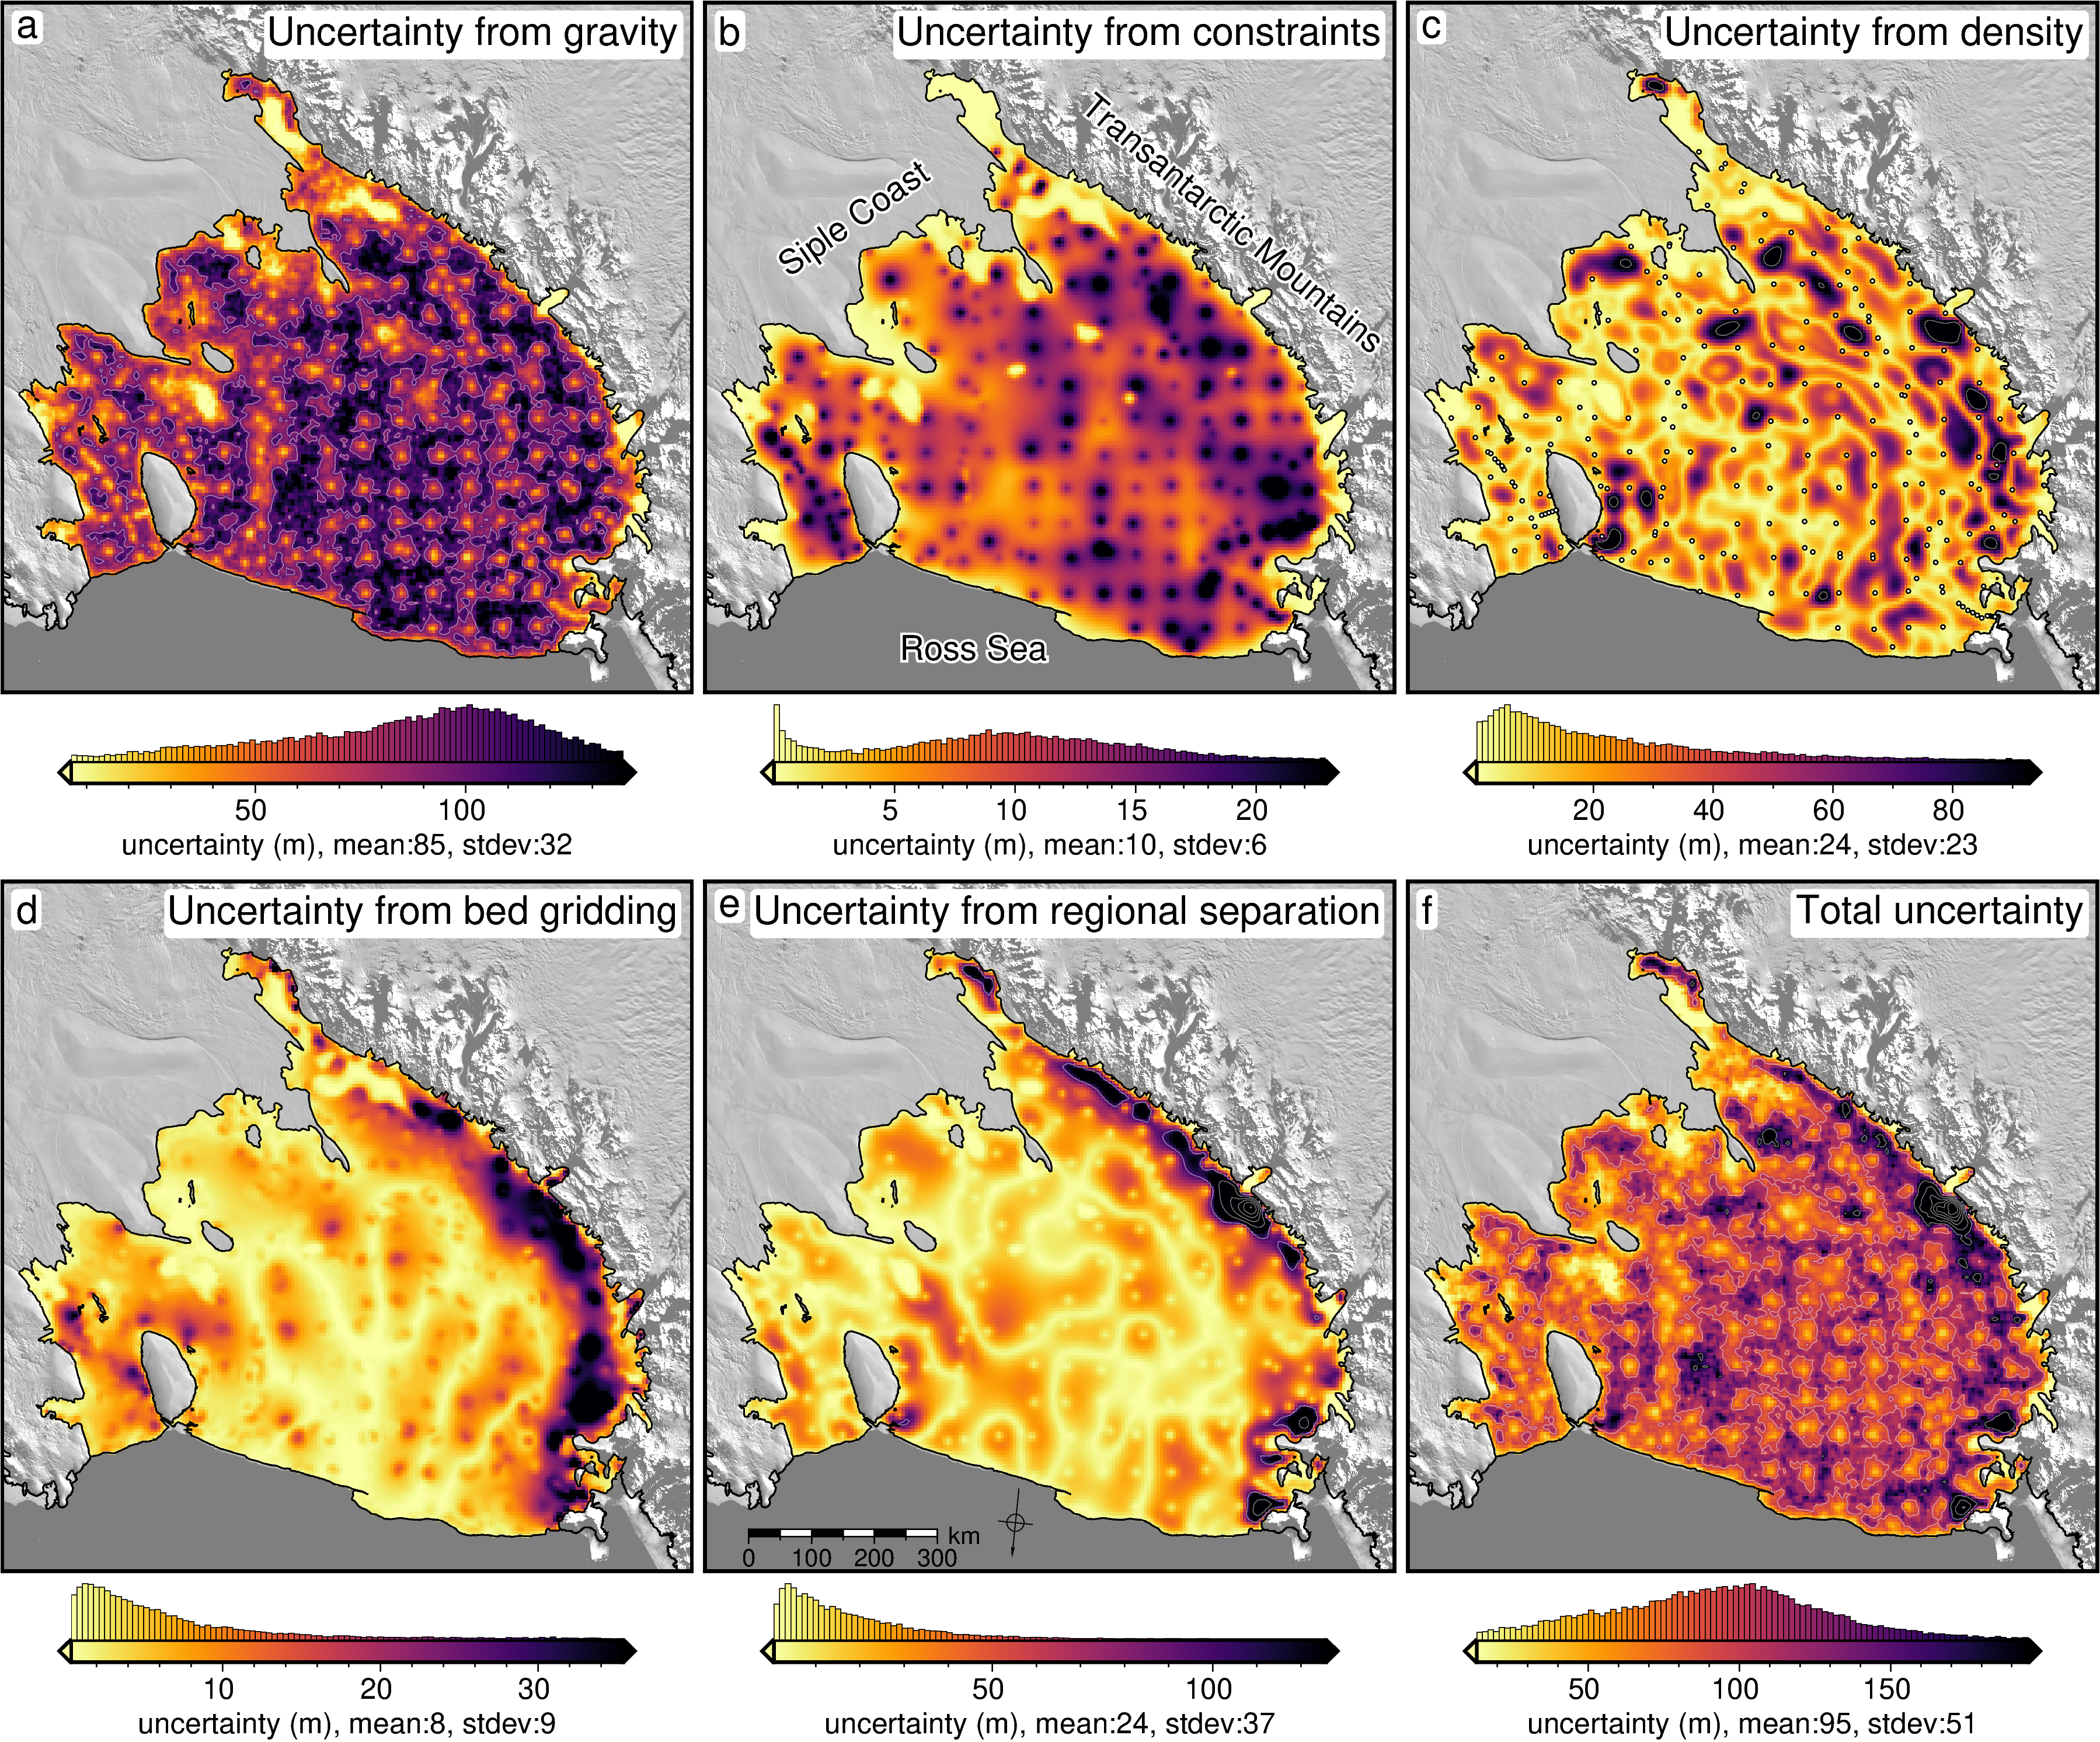
\includegraphics[width=.98\textwidth]{figures/chp4/RIS_MC_sensitivities.png}
    \caption[Monte Carlo results]{Sensitivity analysis for the inversion input data and parameters. Cell-specific weighted standard deviations of the inverted bathymetry results from Monte Carlo simulations with sampling the uncertainties of the \textbf{a)} gravity data, \textbf{b)} constraint points depths, \textbf{c)} ice, water, and sediment density values, \textbf{d)} starting bed interpolation tension factor, and \textbf{e)} tension factor for interpolating the regional gravity component. \textbf{f)} The total uncertainty from the full simulation. 100~m contours in white. Constraints within the ice shelf are shown as dots in \textbf{c}. Grounding line and coastline shown in black \citep{morlighemmeasures2022}. Background imagery is from \citet{scambosmodisbased2007}.}
    \label{fig:chp4_RIS_MC_sensitivity}
\end{figure}

The final bathymetry and uncertainty grids were resampled to a resolution of 500~m, from their original 5~km resolutions, masked outside of the ice shelf, and merged to the 500~m resolution bed and uncertainty data of BedMachine v3. This final bathymetry has a mean elevation of $\sim$-700~m within the ice shelf. The deepest point is $\sim-1370\pm187$~m, located near the Byrd Glacier outlet (Figure \ref{fig:chp4_inversion_inputs}b). Bathymetric features appear to have continuity with features from BedMachine v3 data outside of the ice shelf. The RMS difference between the bathymetry and the original constraint point depths is 44~m. Subtracting the bathymetry from the ice base elevations of BedMachine v3 \citep{morlighemdeep2020, morlighemmeasures2022} gives the water column thickness, as shown in Figure \ref{fig:chp4_RIS_inversion_profiles}b. Without ice base uncertainty estimates from BedMachine v3, we use the bathymetry uncertainty as our uncertainty for the water column thickness, acknowledging that this is a minimum uncertainty. Within the ice shelf boundary, this water column thickness has a mean value of 260~m and a maximum of 1000~m, located near the Nimrod Glacier outlet. Here, the bathymetry has an uncertainty of $\pm$800~m. Outside of this region, the thickest ocean cavity is $\sim940\pm180$~m, located at the Byrd Glacier outlet. The similarity between the bathymetry depth and the water column thickness shows that the ocean cavity is predominantly controlled by bathymetry and that the ice base topography is smooth compared to the bed. The uncertainty in the bed elevation ranges from $\sim$10~-~850~m, with a mean of 95~m (Figure \ref{fig:chp4_RIS_inversion_results}b). It has an approximately normal distribution, with a slight skew to the higher values. In general, the uncertainty is lowest at the constraint points and highest far from constraints. There are elevated uncertainties in several spots, with the largest being along the Transantarctic mountain front.\\

\subsubsection{Partitioning uncertainty}

The uncertainty in the inverted bathymetry which arises from the uncertainty in gravity data (Figure \ref{fig:chp4_RIS_MC_sensitivity}a) is relatively spatially uniform, with a mean of 85~m. It is lowest immediately at the constraint points, and generally highest far from constraint points. The uncertainty from the constraint point depths (Figure \ref{fig:chp4_RIS_MC_sensitivity}b) is also generally spatially uniform, with a mean of 10~m. Conversely, it is highest at the constraint points, and lowest far from constraint points. The uncertainty resulting from the choice of density values (Figure \ref{fig:chp4_RIS_MC_sensitivity}c) displays a more heterogeneous spatial distribution than the previous two uncertainties. It is lowest at the constraint points and has a mean of 24~m. The largest values are located at the gaps between constraint points. The uncertainty resulting from the interpolation of the starting bed (Figure \ref{fig:chp4_RIS_MC_sensitivity}d) has a distinct spatial distribution. It is highest along the Transantarctic Mountain front, with values up to 40~m, but it has an overall mean of 7~m. Lastly, the uncertainty resulting from the estimation and removal of the regional component of gravity, prior to the inversion, (Figure \ref{fig:chp4_RIS_MC_sensitivity}e), also shows highest values along the mountain front, with values over 200~m (up to 700~m at the Nimrod Glacier outlet). The mean value is 24~m. The reported uncertainties and their components from a wide range of past studies are shown in Table \ref{table:chp4_past_study_uncertainties}. \\


\begin{table}
\footnotesize 
\centering
\begin{tblr}{
  width = \linewidth,
  colspec = {Q[350]Q[140]Q[155]Q[160]Q[195]},
  cell{1}{2} = {c=4}{0.597\linewidth,c},
  vline{2} = {3-24}{},
  hline{2} = {2-5}{},
  hline{3} = {-}{},
  hline{25} = {-}{},
}
                                  & Inverted bathymetry uncertainty (m) & & &                 \\
Study                             & total  & from gravity  & from geology  & from constraints \\
\textbf{This study} ($\overline{x}\pm1\sigma$) & 95$\pm$51 & 85$\pm$32     & 48$\pm$30    & 10$\pm$6 \\
\citet{eisermannbathymetric2021}   & 220               & 84          & 116        & 20     \\
\citet{tintobathymetry2015}        & 160               & 26          & 124        & 10     \\
\citet{constantinoseafloor2020}    & 133               & 34          & 90         & 5-10   \\
\citet{boghosianresolving2015}     & 110               & 10-28       & 50-70      & 10     \\
\citet{tintoprogressive2011}       & 70                & 34          & 10-15      & 20     \\
\citet{constantinocook2023}        & 69-123            & 32-39       & 27-74      & 10     \\
\citet{tintoross2019}              & 68                & 48          & 10         & 10     \\
\citet{eisermannbathymetry2020}    & 175-225           & -           & -          & 10     \\
\citet{jordannew2020}              & 100               & 23          & -          & -      \\
\citet{anbathymetry2019}           & 60                & 60          & -          & -      \\
\citet{studingerestimating2004}    & 250               & -           & -          & -      \\
\citet{weigetz2020}                & 246               & -           & -          & -      \\
\citet{greenbaumocean2015}         & 190               & -           & -          & -      \\
\citet{brisbourneseabed2014}       & 160               & -           & -          & -      \\
\citet{hodgsonfuture2019}          & 100               & -           & -          & -      \\
\citet{yangbathymetry2021}         & 68                & -           & -          & -      \\
\citet{anbed2017}                  & 60                & -           & -          & -      \\
\citet{millanbathymetry2017}       & 50-65             & -           & -          & -      \\
\citet{millanvulnerability2018}    & 30-50             & -           & -          & -      \\
\citet{millanconstraining2020}     & 45                & -           & -          & -      \\
\citet{filinanew2008}              & -                 & 19          & -          & -      \\
\textbf{Mean}                      & 117 (N=25)        & 40 (N=13)   & 57 (N=11)  & 12 (N=10)
\end{tblr} 
\caption[Bathymetry uncertainties comparison]{Reported inverted bathymetry uncertainties and the various components. Our reported geologic uncertainty is the combination of uncertainties resulting from the density values and the tension factor used in grinding the regional field.}
\label{table:chp4_past_study_uncertainties}
\end{table}

% \citet{constantinoseafloor2020} total of 133 m,  34m from 2.4mgal cross over using bouguer slab, 5-10 from constraints, and 90 from density variations,
% \citet{eisermannbathymetry2020} totals of 175m, 225m, and 210m,
% 10m from ice thickness uncertainty, rest from gravity and density assumptions
% \citet{tintoross2019} 68m total, 48m for 3.2mGal bouguer slab, 10m from constraints, and 3\% (10m) from density
% \citet{jordannew2020} total of 100 m, 23 m from 1.56 mGal crossover and 130 m uncert if using 2500 instead of 2670, 
% \citet{yangbathymetry2021} 68 m 
% \citet{millanconstraining2020} 45 m, 
% \citet{boghosianresolving2015} 110 m, 10-28 m from gravity data, 10m from constraints, 50-70m from density,
% \citet{hodgsonfuture2019} 100 m,
% \citep{anbathymetry2019} 60 m, from 5mGal/100m of water
% \citet{tintobathymetry2015} 160 m total, 124 m from geologic variations, 26m from gravity data, 10 from constraints
% \citet{greenbaumocean2015} 190m total from comparison of grounded ice base from radar and inverted bed 
% \citep{brisbourneseabed2014} 160 m from RMS with constraints
% \citep{weigetz2020} 246 m from comparison of grounded ice base from radar and inverted bed 
% wavelengths resolved by the gravity system, 


\section{Discussion}

Here we discuss the results of our Ross Ice Shelf bathymetry model from the inversion of airborne gravity data. First, we describe the results of the uncertainty and parameter sensitivity analysis. Then we compare our results with two past bathymetry models beneath the Ross Ice Shelf and discuss the differences. Lastly, we discuss various implications of this updated bathymetry model, including how the findings relate to geology, tectonics, and ice sheet dynamics. %Lastly, we suggest future work with aims to improve our understanding of the sub-Ross Ice Shelf bathymetry. 

\subsection{Uncertainties and parameter importance}

The results of our Monte Carlo simulations provide answers to several important questions. 1) Wow confident are we in the inverted bathymetry depths? 2) Where are we most and least confident about the bathymetry depth? 3) What are the specific sources of this uncertainty? and finally, 4) What can be done to limit the uncertainty? Figures \ref{fig:chp4_RIS_MC_results}b and \ref{fig:chp4_RIS_MC_sensitivity}f show the resulting spatial uncertainty of the inverted bathymetry, providing an answer to the first two questions. To determine the sources of this uncertainty, the individual inputs to the inversion were isolated and their effects on the estimated uncertainty were found (Figure \ref{fig:chp4_RIS_MC_sensitivity}).\\

\subsubsection{Gravity component}
 The largest contributor to the overall uncertainty of the inversion is the uncertainty of the gravity data (Figure \ref{fig:chp4_RIS_MC_sensitivity}a). This uncertainty resulting from the gravity data results in a base-level bathymetry uncertainty of $\sim$~85~m and is relatively spatially uniform. This is because each gridded gravity data point is contaminated with independent noise of varying levels during the Monte Carlo sampling. It is this point-by-point random noise that creates the noisy component in the final inverted bathymetry. In reality, the uncertainty of nearby gravity data is likely correlated, where entire lines, or sections of lines have similar uncertainty values, due to changing data collection conditions, like turbulence, or mis-levelling, causing values of entire lines to be offset, or tilted. Here our estimate of gravity uncertainty is entirely dependent on cross-over misties; likely an oversimplified estimation of uncertainty for an entire survey. This suggests that the true uncertainty resulting from the gravity data likely has a different spatial distribution and may be larger than we report; a finding which is not surprising, since the entire method depends on these data.\\ 

\subsubsection{Constraints component}
 The uncertainty in the other data input to the inversion, the constraint point depths, has only a small effect on the results (Figure \ref{fig:chp4_RIS_MC_sensitivity}b). It is worth noting that while the uncertainty resulting from the constraint point measurement uncertainty is low, the constraints themselves are fundamental to the inversion. These constraints feed into all the components of the inversion and thus affect the uncertainty of each component, including the uncertainty from the gravity data. This is shown by the correlation between uncertainty and the distance to the nearest constraint (Figure \ref{fig:chp4_RIS_weighting_grid}) of all the components of Figure \ref{fig:chp4_RIS_MC_sensitivity}. Our Monte Carlo sensitivity analysis only tests the effects of estimated noise in the inputs, and not their overall importance for the inversion. Since the uncertainty in the constraints only impacts the inversion in the immediate vicinity of the constraint, for constraint data collection, efforts should be focused on quantity over quality, assuming the uncertainty can be limited to a reasonable amount. In practice, for over-ice seismic surveying, this may lead to the choice of fast and efficient systems as opposed to high-resolution systems, if the main goal of the survey is to collect bathymetry constraints. For example, towable snow streamers and sources such as surface detonations or vibroseis \citep[e.g.,][]{hofstedeevidence2021, smithdetailed2020} can collect data very efficiently ($\sim20$~km/day), compared to higher-resolution surveys with buried geophone arrays and drill-emplaced explosives \citep[e.g.,][]{horgansediment2013}. The remaining sources of uncertainty are related to user-defined inversion parameters.\\

\subsubsection{Density component}
The choice of density values for the ice, water, and sediment results in a mean uncertainty in the bathymetry model of 24~m (Figure \ref{fig:chp4_RIS_MC_sensitivity}c). The ranges of densities tested in the Monte Carlo simulation were $\sim$ 905~-~925~kg~m\textsuperscript{-3} for ice\footnote{We note that the maximum density of meteoric ice is 917~kg~m\textsuperscript{-3}, however; the inclusion of marine ice may raise this value \citep{frickerdistribution2001}}, $\sim$ 1015~-~1035~kg~m\textsuperscript{-3} for seawater, and $\sim$~1600~-~3000~kg~m\textsuperscript{-3} for the seafloor. We only test homogeneous changes in the density values.\\

The uncertainty arising from the choice in density values has a strong spatial correlation with the absolute value of the inversion's input gravity, the residual gravity (Figure \ref{fig:chp4_RIS_terrain_regional_residual}d). This correlation can be explained by the inverse relation between the amplitude of the corrections applied to the bathymetry during the inversion, and the density contrasts used in the inversion. For the same gravity anomaly, a smaller density contrast results in a larger amplitude correction while a larger density contrast results in a smaller correction. This means that changes in the density values just affect the amplitude of the correction applied to the bathymetry. Often, spatially variable density is used as a means to account for the regional component of gravity \citep[e.g.,][]{tintoross2019, constantinoseafloor2020}. We note that there is an additional benefit to incorporating spatially variable densities. If adequate \textit{a priori} information is known to justify a density distribution, this can be used to allow differing amplitudes of corrections across the inversion domain. In other words, if the seafloor truly is denser in one region of the inversion compared to the seafloor elsewhere, for a similar gravity anomaly, the inversion correction should be of smaller amplitude in the high-density region. However, due to a lack of geologic knowledge beneath the ice shelf, we use constant density values. We propose Monte Carlo sampling of a wide range of possible density values as a robust and feasible method to avoid biasing the resulting bathymetry model to either too high or too low correction amplitudes, to achieve both the most realistic results and an estimation of the uncertainty.\\

\subsubsection{Interpolation component}
The final components of the overall uncertainty are related to interpolation conducted during two stages of the inversion; 1) the interpolation of the starting model from the sparse constraint point depths, and 2) the estimation of the regional field from the interpolation of gravity values at the constraint points. Here, we have used a minimum curvature gridding algorithm \citep{smithgridding1990}, which accepts a tension factor for the interpolation which can range from 0 to 1. Figure \ref{fig:chp4_starting_bed_comparison} shows the results of six different values of this tension factor for creating the starting bed model. These figures show that low values of tension are able to accurately reproduce the data with a smooth interpolation, but can result in unconstrained local maxima or minima. Conversely, high tension values produce smooth surfaces without false oscillations but don't adhere to the data as well. For these issues associated with the two end members, intermediate values of 0.25 and 0.35 are often suggested for potential field data and topographic data, respectively. We suggest a more robust alternative to using these suggested values is the Monte Carlo sampling approach we have used. This runs the inversion with a variety of tension factors and uses the standard deviation of the resulting bathymetry models as a means to estimate the uncertainty associated with the choice of the tension factor. While tensioned minimum curvature gridding has been used in several past inversions \citep[e.g.,][]{yangbathymetry2021, millanconstraining2020, anbathymetry2019}, the choice of the tension values has not been discussed for these applications. \\ 

The uncertainties arising from the choice of tension factors are shown in Figure \ref{fig:chp4_RIS_MC_sensitivity}d and e. The tension factor for gridding the starting bed model results in a relatively low uncertainty with a mean of 7~m. The resulting uncertainty for the regional separation is comparatively high, with a mean of 24~m. Both of these results show large spatial heterogeneity, with significantly larger uncertainties along the Transantarctic Mountain front. This is likely related to the poor performance of this gridding algorithm for high-gradient data. This region along the mountain front has both steep topography and high amplitude gravity anomalies. \\

\subsubsection{Reducing uncertainties}

Of the various components of the uncertainty analysis, only some can feasibly be reduced. Reducing the uncertainty resulting from the interpolation parameters may be possible with future method development, but this is beyond the discussion of this research. To our knowledge, there is no robust method of determining a spatially variable density distribution to be used in the inversion, without the collection of in-situ data. This leaves the data inputs, gravity and constraints, as viable components of a bathymetry inversion where further reductions of uncertainties can occur. We propose a favourability of quantity over quality for constraint data since typical bed elevation uncertainty is already relatively low, and therefore more data of mediocre quality should be prioritized over high-quality but spatially limited data. In order to reduce the uncertainty component resulting from the gravity data, first we must be able to estimate the realistic spatial uncertainty of the gravity data itself. A simple cross-over analysis is too simple to cover the effects of turbulence, changing flight speed and altitude, and errors in processing steps, such as base station ties and levelling. The areas of largest uncertainty are generally a function of 1) distance to the nearest constraint point (Figure \ref{fig:chp4_RIS_weighting_grid}) and 2) proximity to steep gradients of topography and/or gravity (Figure \ref{fig:chp4_RIS_MC_sensitivity}d and e). This highlights the entire Transantarctic Mountain front of the Ross Ice Shelf and the two major constraint gaps in the central-east portion of the ice shelf (Figure \ref{fig:chp4_RIS_weighting_grid}) as locations that would greatly benefit from additional seismic surveying. 

\subsubsection{Past estimations of uncertainty}

Our comprehensive uncertainty and sensitivity analysis is shown to be similar to the approximated uncertainties reported for other ice shelves (Table \ref{table:chp4_past_study_uncertainties}). Some differences include; our reported uncertainty resulting from the gravity data uncertainty is the highest reported, while our values resulting from other sources, and the total uncertainty, were similar to those of other studies. Our larger reported uncertainty resulting from the gravity data likely shows that the simple Bouguer slab approximation used by the other studies underestimates the component of uncertainty resulting from the gravity data uncertainty. We take the uncertainties resulting from geologic variations to be the combination of our reported uncertainties from the chosen density values (Figure \ref{fig:chp4_RIS_MC_sensitivity}c) and from the regional separation gridding (Figure \ref{fig:chp4_RIS_MC_sensitivity}e) since these both affect the estimation of the regional component. The uncertainty resulting from the constraint point measurement uncertainty was very similar across all studies.\\

From this, we propose future bathymetry inversions undertake similar uncertainty analysis through the Monte Carlo sampling of the input parameters. This technique not only provides similar uncertainty estimates to past studies, but it accomplishes it in a systematic and reproducible method. Additionally, this technique provides a spatial distribution of the uncertainties, instead of a single value. Once the inversion workflow is set up, the sampling and re-running of the inversion is a simple procedure, and with the use of Latin hypercube sampling, we have shown that with only 10 runs, the parameter space of all the inputs is adequately sampled (Figure \ref{fig:chp4_latin_hypercube_sampling}).\\

\subsection{Past bathymetry models}

Our gravity-inverted bathymetry model for the sub-Ross Ice Shelf reveals significant differences with previous bathymetry models. However, a portion of these differences are not related to the inversion, but to the creation of the starting model. First, we will discuss the differences between our starting bathymetry model and another interpolation-based bathymetry model, then we will compare our inversion results with two past models. These past models include Bedmap2 \citep{fretwellbedmap22013} and Bedmachine v3 \citep{morlighemdeep2020, morlighemmeasures2022}. The Bedmap2 model for the Ross Ice Shelf region is created from the interpolation of the same constraint points within the ice shelf as used in this study, as well as grounded ice thickness measurements and limited rock outcrop elevation data \citep{fretwellbedmap22013, lebrocqimproved2010, timmermannconsistent2010}. BedMachine v3 used these point measurements and applied additional methods to increase the resolution of the bed. For outside of the ice shelf, this included mass conservation for areas of fast-moving ice (outlet glaciers and ice streams), streamline diffusion for regions of slow-moving ice, as well as minimum curvature gridding to interpolate the remaining gaps \citep{morlighemdeep2020}. Within the ice shelf, BedMachine used the gravity inversion results of \citet{tintoross2019}.\\

\subsubsection{Starting model comparison}

Figure \ref{fig:chp4_starting_bed_comparison} shows the series of six starting bed models we created from the interpolation of the sparse constraints. These were created with six levels of tension applied to a minimum curvature interpolation. The cell-specific standard deviation of these six models shows the uncertainty associated with this interpolation (Figure \ref{fig:chp4_starting_bed_comparison}g), and the mean of the six grids is our chosen starting model (Figure \ref{fig:chp4_starting_bed_comparison}h) This is compared with the Bedmap2 model in (Figure \ref{fig:chp4_starting_bed_comparison}i). The RMS difference between the two grids, within the ice shelf, is 95~m. Our starting bed is deeper proximal to the entire grounding zone, while it is shallower along the ice front and throughout the centre of the ice shelf. However, these differences of up to 200~m do not suggest our starting model is inaccurate. Sampling the grid values at the constraint points and comparing them with the constraint depths shows that our model was significantly better at adhering to these constraints, compared to Bedmap2. The RMS of the difference with our model was 14~m, while the RMS of Bedmap2 was 138~m (Figure \ref{fig:chp4_inversion_inputs}).\\

These large differences for Bedmap2 are concentrated along the Transantarctic Mountain front, where the interpolation algorithm used in Bedmap2 resulted in excessively shallow bathymetry. This interpolation appears to have favoured smoothness over accuracy for this location of steep terrain. This has resulted in a "leakage" of the high elevations within the mountains into the bathymetry interpolation, as pointed out in this region \citep{lebrocqimproved2010}, as well as for other ice shelves \citep{brisbourneupdated2020}. This over-smoothing and "leakage", while strongest along the mountain front, can be seen along the entire grounding zone. This is the reason why Bedmap2 was shallower than our starting model along the grounding line. This shows that care needs to be taken when picking or creating a starting model for an inversion, especially in regions of steep topography. The re-creation of the starting model from the point data allows the choice of interpolation techniques better suited for the region of interest, compared to techniques determined most suitable for a continent-wide study.\\

\subsubsection{Inversion result comparisons}

\begin{figure}[!ht]
    \centering
    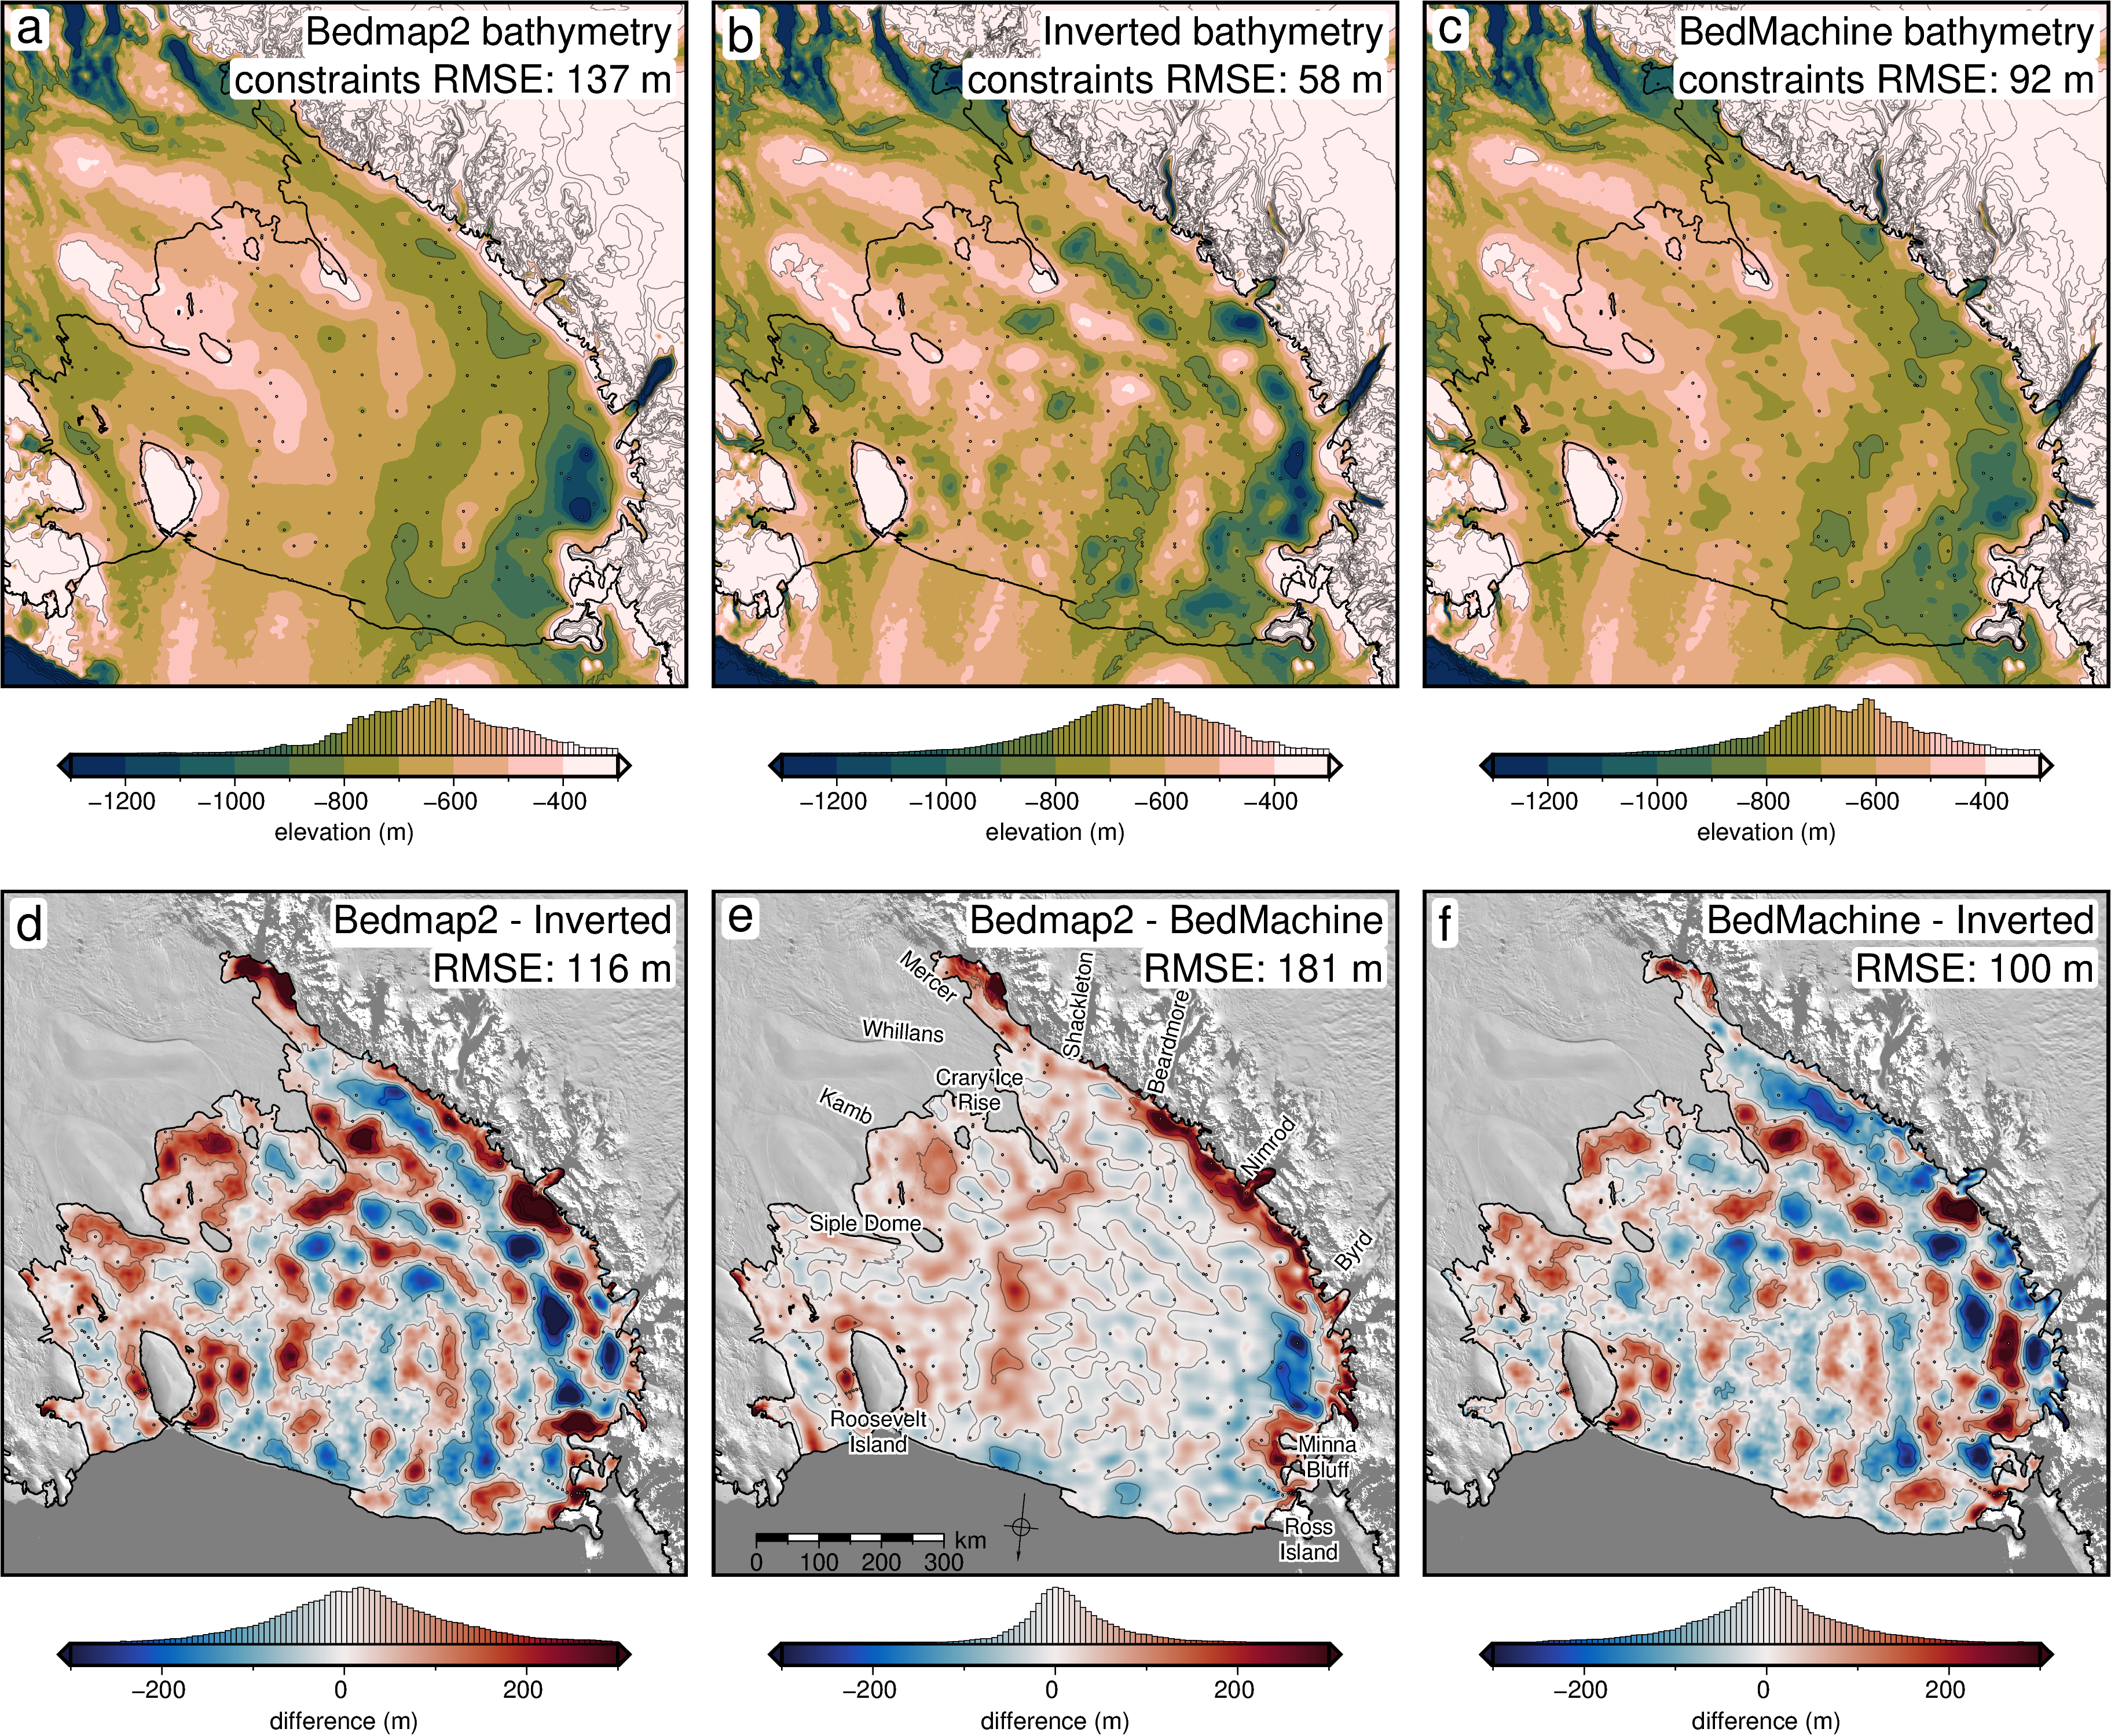
\includegraphics[width=.98\textwidth]{figures/chp4/RIS_bed_model_comparisons.png}
    \caption[Inverted bathymetry comparisons]{Comparison of our inverted bathymetry with past models. \textbf{a)} Bedmap2 bathymetry, \textbf{b)} our inversion results, from the weighted mean of the full Monte Carlo simulation, and \textbf{c)} BedMachine bathymetry. All three share the same colour scale and are contoured at 400 m intervals. RMS difference with the constraint points for each model is stated on the maps. \textbf{d)} Difference between our model and Bedmap2, \textbf{e)} difference between Bedmap2 and BedMachine v3, and \textbf{f)} difference between our model and BedMachine v3. Grids share a colour scale and are contoured at 100 m intervals. Blue regions in \textbf{d} and \textbf{f} indicate where our results are shallower, while red regions indicate where our results are deeper than the past models. Blue regions in \textbf{e} indicate where BedMachine is shallow, while red regions indicate where BedMachine is deeper than Bedmap2. RMS differences are stated on the maps. Grounding line and coastline are shown in black \citep{morlighemmeasures2022}. Background imagery is from \citet{scambosmodisbased2007}. Elevations are referenced to the WGS-84 ellipsoid.}
    \label{fig:chp4_RIS_bed_model_comparison}
\end{figure}

\paragraph*{Bedmap2 comparison}

Figure \ref{fig:chp4_RIS_bed_model_comparison} compares our final bathymetry results with the models of Bedmap2 and BedMachine v3. Additionally, several profiles across different regions are shown in Figure \ref{fig:chp4_RIS_inversion_profiles}, comparing the various models. Interestingly, the inversion has raised the RMS difference with Bedmap2, compared to the starting model. But due to the issues with the Bedmap2 grid along the mountain front, this increased difference is expected. The differences between our inverted bed and Bedmap2 have a normal distribution (Figure \ref{fig:chp4_RIS_bed_model_comparison}d). Our results introduce many small-scale features, as expected since Bedmap2 is an inherently smooth product. However, there are several noticeable large-scale differences with Bedmap2. Proximal to the grounding line, our results are generally deeper, as seen with the starting model comparison (Figure \ref{fig:chp4_RIS_inversion_profiles}g). Many of the regions where our results are deeper are related to the issue of over-shallow interpolation of Bedmap2. Portions of the grounding zone along the Siple Coast are over 200~m deeper, including the Kamb (Figure \ref{fig:chp4_RIS_inversion_profiles}c) and Mercer ice stream grounding zones. \\

Another notable difference is an NW-SE oriented trough which appears in our results but is essentially absent in Bedmap2. This feature begins at the southern end of the Crary Ice Rise grounding zone and continues $\sim300$~km, paralleling the mountain front (Figure \ref{fig:chp4_RIS_inversion_profiles}c). This feature is the southwestern-most of a series of 2 or 3 parallel troughs and ridges, as shown in Figure \ref{fig:chp4_RIS_inversion_profiles}d. These features are oriented at a high angle to both E-W and N-S flight lines, increasing their likelihood as true features of the bathymetry and not flight line levelling artifacts. While they are subtle, their presence alters the general \textit{texture} in the region from a primary N-S / NNE-SSW to an NW-SW orientation. This switches the general trend of bathymetry features in the region to be aligned with Siple Coast ice flow, rather than the Transantarctic outlet glacier ice flow. Whether these bedforms are tectonic in nature, revealing the tectonic fabric, or are erosion/depositional, and thus revealing the past flow directions of the previously grounded ice sheet is unknown. The last major difference with Bedmap2 is a significantly deeper bathymetry along the western edge of Roosevelt Island (Figure \ref{fig:chp4_RIS_inversion_profiles}a).\\


\paragraph*{Bedmachine comparison}

Comparing our results to Bedmachine v3 provides a unique opportunity to evaluate the differences resulting from different gravity inversion algorithms. The gravity inversion results of \citet{tintoross2019}, which comprise the Bedmachine v3 data beneath the ice shelf, used similar input datasets (gravity data and constraint points), suggesting that differing inversion algorithms and workflows are likely responsible for the majority of the differences shown in Figure \ref{fig:chp4_RIS_bed_model_comparison}f. However, some of the differences may arise from re-processing the gravity data, and a different method of gravity reduction applied here, as compared in Section \ref{chp4:past_inversions}.\\

% Additionally, we have incorporated additional constraint points. These include the Little America Station Byrd Trail seismic survey (1958) between Roosevelt Island and King Edward VII peninsula, the Victoria Land Traverse (1958-59) and the Discovery Deep Traverse (1960), from Roosevelt Island across the ice front to the Skelton Glacier, and the Ross Ice Shelf Traverse (1957-58), a large traverse encompassing most of the ice shelf in a triangle between Roosevelt Island, Minna Bluff, and Crary Ice Rise. See \citet{bennettgravity1964} for descriptions of these traverses.

To remove the regional component of gravity, \citet{tintoross2019} used a smoothly varying density model in their inversion. To create this density model, they created an initial prism layer with prisms extending from their starting bathymetry to a depth of 60~km. With the gravity disturbance, they performed a density inversion to recover the density of each prism. This spatially variable density was then low-pass filtered, with a 50~km cutoff. Incorporating this remaining long-wavelength gravity signal within the density model removed the regional component from the gravity input to the inversion. This technique is conceptually similar to high-pass filtering the gravity data to remove the long-wavelength component. For the inversion, \citet{tintoross2019} used the commercial software Geosoft Oasis Montaj. Limited information is available from Geosoft as to the specifics of this inversion procedure.\\

Comparing our bathymetry (Figure \ref{fig:chp4_RIS_bed_model_comparison}f), there is a normal distribution of differences, centred on zero. The RMS difference between the two grids is $\sim$100~m. Comparing each grid to the constraint point depths, the BedMachine grid has an RMS difference of 92~m, compared to our RMS of 44~m. Generally, our results are approximately 50-100~m deeper proximal to most of the Siple Coast grounding line. Conversely, our results are approximately 50-100~m shallower along the Transantarctic Mountain front. This could be due to our inability to fully fix the issue of overly-shallow interpolation of data along the mountain front in the creation of our starting model, as discussed.\\

Alternatively, the differences could be a result of the different gravity reduction steps. Figure \ref{fig:chp4_RIS_terrain_regional_residual}b and e show that correcting the gravity disturbance for the terrain mass effect results in a large negative topo-free disturbance along the Transantarctic Mountain front (dark blues in \textbf{b}). During the regional field estimation, fitting a spline to these large negative values would bring down the nearby regional field, resulting in an underestimation of the regional (more negative), and thus an overestimation of the residual (positive values). This is shown by the profile of Figure \ref{fig:chp4_RIS_terrain_regional_residual}e. On the right side, along the mountain front, in an attempt to fit the negative values of the topo-free disturbance (red dashed line), the regional field (blue) has been underestimated, leaving a large positive residual anomaly (pink dashed). This positive residual results in a shallowing of the inverted bathymetry.\\

\begin{figure}[p]
% \renewcommand\thesubfigure{\arabic{subfigure}}
  \centering
    \begin{subfigure}[t]{.8\textwidth}
        \includegraphics[width=\textwidth]{figures/chp4/RIS_profile_locations.png}
    \end{subfigure}
    
    \makebox[\linewidth][c]{%
    \begin{subfigure}[t]{.6\textwidth}
        \includegraphics[width=\textwidth]{figures/chp4/profile_A.png}
    \end{subfigure}
    \begin{subfigure}[t]{.6\textwidth}
        \includegraphics[width=\textwidth]{figures/chp4/profile_B.png}
    \end{subfigure}
    }
    \makebox[\linewidth][c]{%
    \begin{subfigure}[t]{.6\textwidth}
        \includegraphics[width=\textwidth]{figures/chp4/profile_C.png}
    \end{subfigure}
    \begin{subfigure}[t]{.6\textwidth}
        \includegraphics[width=\textwidth]{figures/chp4/profile_D.png}
    \end{subfigure}
    }
    \makebox[\linewidth][c]{%
    \begin{subfigure}[t]{.6\textwidth}
        \includegraphics[width=\textwidth]{figures/chp4/profile_E.png}
    \end{subfigure}
    \begin{subfigure}[t]{.6\textwidth}
        \includegraphics[width=\textwidth]{figures/chp4/profile_F.png}
    \end{subfigure}
    }
    \begin{subfigure}[t]{.95\textwidth}
        \includegraphics[width=\textwidth]{figures/chp4/profile_G.png}
    \end{subfigure}
    
  \caption[Ross Ice Shelf assorted cross-sections]{\textbf{Upper panel)} Ross Ice Shelf inverted bathymetry (left) and water column thickness (bed to ice base) relative to Bedmachine v3 ice base \citep{morlighemmeasures2022}. Pink lines show profile locations with ticks every $\sim$100~km. Grounding line and coastline in black \citep{mouginotmeasures2017}. Constraint points shown as dots. \textbf{Profiles A-G)} Various cross-sections showing the ice layer (light blue), water layer (darker blue), and bathymetry (yellow), with uncertainties (brown). Red and black lines show Bedmap2 and BedMachine v3 bathymetry, respectively. The colour of the ice surface indicates the distance to the nearest constraint. Legend and colourmap shown above profile A.}
    \label{fig:chp4_RIS_inversion_profiles}
\end{figure}

These shallower depths along the mountain front, instead, could be revealing a flaw in the constraint point minimization assumption of the residual being 0 at constraint points. While the constraint point itself doesn't contribute to the residual signal, since the actual bed is equal to the starting bed at those points, deviations between the actual bed and the starting bed in the vicinity of the constraints may lead to a non-zero residual at the constraint. In this case, the interpolation of the regional field attempts to smoothly connect extremely negative values at the mountain front, and high values at the nearby constraint points. This high gradient leads to poor interpolation. This can be seen in \ref{fig:chp4_RIS_terrain_regional_residual}e where the regional (blue line) is forced exactly equal to the topo-free disturbance (red dashed line) at the constraint point at 700~km along the profile. In reality, the residual gravity at that constraint is likely non-zero. A non-zero value may allow the regional field to more closely match the large positive topo-free disturbance located at 720~km.\\

The remaining major differences between our results and BedMachine v3 include the same series of alternating NW-SE troughs and ridges as discussed above, an $\sim$100~m deeper region on the west side of Roosevelt Island, and a significantly deeper ($\sim$250~m) trough spanning from the south side of Minna Bluff to the outlet of the Byrd Glacier. The greatest depths we model in this trough are $\sim1350\pm100$~m, located offshore of the Byrd Glacier Outlet. Preliminary results of a seismic survey at Discovery Deep, just south of Minna Bluff (cyan line Figure \ref{fig:chp4_RIS_MC_results}), in the 2021/2022 field season report depths up to 1450~m (pers. comm. Prof. A. Gorman). These findings confirm the presence of depths of this magnitude. However, our deepest location is approximately 100~km south of the Discovery Deep survey. These seismic data were not included in this inversion. An additional comparison to a seismic survey can be made proximal to the Kamb Ice Stream grounding zone (cyan line Figure \ref{fig:chp4_RIS_MC_results}). \citet{horganpoststagnation2017} image bathymetry depths along a $\sim20$~km seismic survey with a mean depth of $\sim605$~m. Sampling our bathymetry and uncertainty along this profile yields a mean depth of $\sim608\pm45$~m, while sampling BedMachine v3 bathymetry and uncertainty yields a mean depth of $\sim572\pm79$~m.\\

Comparing the various difference maps of Figure \ref{fig:chp4_RIS_bed_model_comparison} shows that our inversion has resulted in more varied topography across the ice shelf compared to \citet{tintoross2019}. This increased amplitude is likely due to the differences in densities used between the inversions. \citet{tintoross2019} used a spatially variable density model, which ranged from $\sim$2600~-~2800~kg~m\textsuperscript{-3}, with a mean of $\sim$2700~kg~m\textsuperscript{-3}. While we used a spatially-constant density value, in the Monte Carlo analysis the density was varied between $\sim$1800~-~3000~kg~m\textsuperscript{-3}, with a mean of $\sim$2400~kg~m\textsuperscript{-3}. This $\sim$300~kg~m\textsuperscript{-3} difference between the mean density values would result in a more subdued inverted bathymetry from the \citep{tintoross2019} model. While the \citet{tintoross2019} density model does a good job of removing the regional field prior to the inversion, whether or not the density values used are representative of the seafloor is questionable. The lowest values in their model of approximately 2600~kg~m\textsuperscript{-3} represent the upper end of sedimentary rock densities \citep{schöndensity2015}, and are significantly greater than expected densities of unconsolidated sediments. For a region with an expected continuous drape of seafloor sediments \citep[Chapter \ref{ch:2},][]{tankersleybasement2022}, we expect the densities used in \citep{tintoross2019} were too high. This explanation for the differences between the inversion results is supported by the strong correlation between our bathymetry uncertainty resulting from the choice in density (Figure \ref{fig:chp4_RIS_MC_sensitivity}c) and the difference between the inversion results (Figure \ref{fig:chp4_RIS_bed_model_comparison}f). This shows the importance of picking a plausible density value, and the added benefit of testing many values to estimate the uncertainty related to the chosen density value. \\


\subsubsection{Ocean cavity comparison}

Due to the smoothness of the base of an ice shelf, relative to bathymetry, the water column thickness beneath many ice shelves is predominately determined by the bathymetry. We use BedMachine v3 ice base elevations and our updated bathymetry to calculate the water column thickness beneath the Ross Ice Shelf and compare the results to the water column thicknesses of Bedmap2 and BedMachine (Figure \ref{fig:chp4_RIS_ocean_draft_comparison}). These differences are very similar to those described above, due to the smooth nature of the ice base. Notable areas where our results show a thicker ocean cavity (within uncertainty ranges) compared to past models include;
\begin{enumerate}
    \item 
    Nearby the Kamb grounding zone ($\sim100\pm50$~m thicker, Figure \ref{fig:chp4_RIS_inversion_profiles}c near km 100).
    \item 
    The west side of Crary Ice Rise ($\sim300\pm150$~m thicker, Figure \ref{fig:chp4_RIS_inversion_profiles}c near km 350).
    \item 
    The south side of Minna Bluff ($\sim300\pm200$~m thicker, Figure \ref{fig:chp4_RIS_inversion_profiles}g near km 2100).
    \item 
    The west side of Roosevelt Island ($\sim200\pm100$~m thicker, Figure \ref{fig:chp4_RIS_inversion_profiles}a near km 220)).
\end{enumerate}

Notable areas where our results show a thinner cavity include;
\begin{enumerate}
    \item 
    The mountain front north of Byrd Glacier ($\sim300\pm50$~m thinner, Figure \ref{fig:chp4_RIS_inversion_profiles}g near km 2000)).
    \item 
    Three 50~km wide regions in the central ice shelf, which are up to $200\pm50$~m thinner.
    \item 
    Several points approximately 50~km off of the Transantarctic Mountain front which are up to $400\pm50$~m thinner (Figure \ref{fig:chp4_RIS_inversion_profiles}c near km 450).
\end{enumerate}

\begin{figure}[!ht]
    \centering
    \includegraphics[width=.98\textwidth]{figures/chp4/RIS_ocean_draft_comparison.png}
    \caption[Water column thickness comparisons]{Comparison of our updated water column thickness with past models. \textbf{a)} Difference between our model and the water column thickness from Bedmap2, and \textbf{b)} the Bedmap2 water column thickness. \textbf{c)} Water column thickness calculated as the difference between BedMachine v3 icebase and our inverted bathymetry. \textbf{d)} Difference between our model and the water column thickness from Bedmachine v3, and \textbf{e)} the Bedmachine v3 water column thickness. Blue regions in the difference maps indicate where our results' water column is thinner, while red regions indicate where our results are thicker than the past models. Grounding line and coastline are shown in black \citep{morlighemmeasures2022}. Background imagery is from \citet{scambosmodisbased2007}. Water column thickness grids are contoured at 200~m intervals, and the 20~m contour is shown in bright blue. The difference grids are contoured at 100~m intervals. Water column thickness grids and difference grids share common colour scales.}
    \label{fig:chp4_RIS_ocean_draft_comparison}
\end{figure}

\subsection{Implications}

Here, we discuss several of the important implications of our updated sub-RIS bathymetry. These implications relate to the stability of the Ross Ice Shelf, geology, and tectonics. 

\subsubsection{New potential pinning points}

We have identified several areas of thin water column thickness ($<20$~m) with our updated results beneath the Ross Ice Shelf. These areas are shown by the 20~m water column thickness contour, in bright blue in Figure \ref{fig:chp4_RIS_ocean_draft_comparison}a. These include a $\sim$100x100~km region SW of Roosevelt Island, several $\sim$50x50~km regions on the north flank of Crary Ice Rise (Figure \ref{fig:chp4_RIS_inversion_profiles}g at km~$\sim900$), and a widespread region south of Crary Ice Rise (Figure \ref{fig:chp4_RIS_inversion_profiles}g at km~$\sim1350$). Thin water depths south of Crary Ice Rise have also been modelled by a local gravity survey along the Whillans Ice Stream grounding zone \citep{mutobathymetry2013}. Additionally, two smaller regions of sub-20~m water column thickness are found nearer the centre of the ice shelf. One is approximately 100~km off the point of Crary Ice Rise and is $\sim400$~km\textsuperscript{2} (Figure \ref{fig:chp4_RIS_inversion_profiles}c at km~$\sim200$). The second is $\sim200$~km north of Crary Ice Rise and is slightly smaller (Figure \ref{fig:chp4_RIS_inversion_profiles}b at km~$\sim350$). None of these shallow water column regions are present in either of the past models. Interestingly, these regions coincide with some of the lowest uncertainties we report $\sim20$~m. A portion of this low uncertainty may be related to the inversion constraining the bathymetry to the ice base, which in regions of thin water column will reduce the variability of the suite of inversions in the Monte Carlo simulation which were used to define the uncertainty.\\

These newly-identified shallow regions highlight where the Ross Ice Shelf was likely grounded in the recent past, or could likely become re-grounded in the future. While some of these regions are small, analysis of pinning points on the Ross Ice Shelf has shown some of the smallest pinning points can create the largest effective resistance on the ice shelf \citep{stillmechanical2019}. Additionally, some of these locations (north side of Crary Ice Rise) are predicted to have on the order of 1~m/yr of basal accretion \citep{adusumilliinterannual2020}. An already thickening shelf within $\sim$20~m of the bed will likely affect the ice sheet dynamics as part of future projections of the ice shelf. Incorporation of these localities of likely past pinning points may aid in resolving the ongoing debate of the style of grounding line retreat and readvance of the Ross Ice Shelf throughout the Holocene \citep{venturellimid2020, kingslakeextensive2018, lowrydeglacial2019}.\\ 


\subsubsection{Basal melting}

\begin{figure}[!ht]
    \centering
    \includegraphics[width=0.95\textwidth]{figures/chp4/RIS_basal_melt.png}
    \caption[Basal melt]{Basal melt rate and water column thickness compared for the Ross Ice Shelf. \textbf{a)} Blue to red contours show interpolated basal melt rate from \citet{dasmulti2020} derived from ROSETTA-ice airborne ice-penetrating radar. Background shows water column thickness from this study. \textbf{b)} Same as \textbf{a} but with basal melt rate from \citet{adusumilliinterannual2020} derived from satellite altimetry. Black line is the grounding line from \citet{mouginotmeasures2017}. Background imagery is from MODIS-MOA \citep{scambosmodisbased2007}.}
    \label{fig:chp4_basal_melt}
\end{figure}

Our updated bathymetry, water column thickness, and uncertainty maps provide additional information vital to understanding the distribution of basal melt beneath the ice shelf. Melt beneath the Ross Ice Shelf is thought to predominantly occur 1) along the ice front, where Antarctic Surface Water causes rapid melting in the summer \citep[Figure \ref{fig:chp4_basal_melt}][]{horgansurface2011, moholdtbasal2014}, and along the deep grounding zones of the Transantarctic Mountain front, where contact with High Salinity Shelf Water induces melting \citep[Figure \ref{fig:chp4_basal_melt}b][]{tintoross2019, adusumilliinterannual2020}. Throughout the centre of the ice shelf are zones of refreezing \citep[Figure \ref{fig:chp4_basal_melt}][]{dasmulti2020, adusumilliinterannual2020}. Overall basal melting of the Ross Ice Shelf is thought to be low compared to other shelves due to the blocking of warm Circumpolar Deep Water from entering the cavity. This blocking is from a layer of dense High Salinity Shelf Water \citep{tintoross2019, dinnimanmodel2011}. The Hayes Bank (Figure \ref{fig:chp4_inversion_inputs}b) has been identified  as one location where the Circumpolar Deep Water is able to penetrate the ice shelf cavity and induce melting, but this penetration is thought to be limited to the region near Roosevelt Island \citep{tintoross2019, dasmulti2020}. Our ocean cavity is $\sim100$~m thicker than \citet{tintoross2019} immediately to the west of Roosevelt Island (Figures \ref{fig:chp4_RIS_inversion_profiles}a and \ref{fig:chp4_RIS_ocean_draft_comparison}d). This region should be investigated with sub-shelf circulation models using our updated bathymetry. Our larger cavity allowing the inflow of warm Circumpolar Deep Water beyond Roosevelt Island could help explain the relatively large basal melt rate found in the region as shown by satellite altimetry (Figure \ref{fig:chp4_basal_melt}b).\\

The high melt rates measured along the Transantarctic Mountain front \citep{adusumilliinterannual2020} are caused by the inflow of High Salinity Shelf Water \citep{tintoross2019}. This water is thought to be guided by bathymetric troughs and is able to induce melting only at large depths, due to the pressure suppression of the melting temperature of ice. Figures \ref{fig:chp4_basal_melt} show a comparison of both airborne radar and satellite altimetry-derived basal melt rates to the updated water column thickness resulting from our bathymetry inversion. The deeper bathymetry proximal to the Transantarctic Mountain front found in both our inversion and \citet{tintoross2019}, compared to the depths of Bedmap2, help explain the high melt rates measured there. The other locations we report with deeper bathymetry near grounding zones, such as the south side of Minna Bluff, and the far southern end of the ice shelf, at the Mercer Ice Stream grounding zone, may be potential locations where High Salinity Shelf Water is able to induce basal melt. Additionally, some of the very shallow water column thicknesses ($<20$~m) we find (Figure \ref{fig:chp4_RIS_ocean_draft_comparison}c), for instance to the south of Crary Ice Rise, correspond with low basal melt rates (Figure \ref{fig:chp4_basal_melt}). This may be due to the lack of stratification in the water column, which occurs due to tidal mixing possible only in thin water columns \citep{mutobathymetry2013, hollandmodel2008}.


% RIS
% RIS show high melt rates under deep ice drafts near GZ and shallow ice drafts near ice front, separated by zones of refreezing \citep{adusumilliinterannual2020}
% most RIS melting at ice drafts between 250 and 750m \citep{adusumilliinterannual2020}
% recent stability of RIS due to insulation of cavity from warm CDW intrusions by cold dense water masses  \citep{tintoross2019, dinnimanmodel2011}
% 25-30\% of total mass loss from basal melt \citep{rignoticeshelf2013}
% mCDW flows south at Hayes Bank to ice front, melting hotspot \citep{dasmulti2020}

% GZ
% RIS basal mass loss driven by cold, High Salinity Shelf Water melting near GZ 
% ocean modelling suggest melt rates are less variable at deep GZ sinze driven by stable circulation of HSSW \citep{tintoross2019}
% ICE FRONT
% 10-40\% sub-RIS melt within 40km of ice front \citep{horgansurface2011}
% ice shelf front melt less important than at grounding since it is within passive ice zones 
% \citep{adusumilliinterannual2020}

% BATHY
% no direct relation between cavity thickness and melting \citep{goldbergbathymetric2020, derydtgeometric2014}
% seabed ridge (300 m )blocks deep and warm waters from reaching thickest ice in Pine Island Glacier. Ridge enhances PIG's sensitivity to oceanic and therefore climatic forcing, by \citep{dutrieuxstrong2014, derydtgeometric2014} 
% similar to entrance sill offshore of ice front at Jakobshavn Glacier

% thin water is tidally mixed, not statified, and therefore has slower basal melting \citep{mutobathymetry2013, holland2008}

% in general grounding line is deeper than bedmap2
% Whillans and Mercer has shallower grounding zones and thinner ocean drafts. 
% 400 m deeper at Nimrod glacier grounding zone Figure \ref{fig:chp4_RIS_inversion_profiles}d 
% 200 m deeper at Mulock glacier grounding zone


\subsubsection{Geologic and tectonic significance}

While there are many interesting implications to explore in this new dataset, we limit our discussion to several sub-Ross Ice Shelf bathymetric features of possible importance to solid-Earth investigations. These features include the bathymetry along the Transantarctic Mountain front, a deep feature on the southwest flank of Crary Ice Rise, and a newly identified orientation of bathymetry features, aligned with the Siple Coast ice streams. 

\paragraph*{Transantarctic Mountain front}

The Transantarctic Mountains (Figure \ref{fig:chp4_inversion_inputs}a) make up the world's largest rift shoulder. Despite their prominence, the uplift mechanisms are still debated \citep{goodgegeological2020}. It is likely that these mechanisms vary along-strike, and consist of some combination of thermal, flexural, or isostatic support \citep{goodgegeological2020}. For the central TAM, a mechanism of cantilevered flexure is proposed for the uplift of the mountains \citep{wannamakeruplift2017, yamasakinumerical2008}. This theoretically should be accompanied by a deep trough parallel just offshore the range front, and an outer bathymetric high, approximately 200 km from the range front \citep{sternflexural1989}. These features have not yet been observed \citep{tenbrinkgeophysical1993, wannamakeruplift2017}. Our results show a deep trough along the range front between the Nimrod Glacier and Minna Bluff, with bathymetry highs further offshore. These features may support the theory of flexural uplift along this portion of the TAM \citep{wannamakeruplift2017}. Further south, where the trough disappears, the mechanism of flexural uplift is not required, since the mountains have a crustal root, which likely provides the uplift mechanism, via Airy isostasy \citep{blockantarctic2009, wannamakeruplift2017}. 

% support lithospheric foundering and the associated thermal support are proposed for the southern TAM \citep{shenseismic2018}, mechanical support through a cantilevered flexure mechanism is proposed for the central TAM \citep{wannamakeruplift2017}, and thermal support associated with a high-temperature anomaly of the upper mantle is suggested for the vicinity of Ross Island \citep{olivettivariability2018}. 

% MT survey \citep{wannamakeruplift2017} shows highly resistive lithosphere of upper mantle, eliminating thernal load possibility, and suggests cantilevered flexure for uplift of CTAM, but lack of hangingwall flexural trough is not observed \citep{tenbrinkgeophysical1993}

\paragraph*{Fault bound Crary Ice Rise}

Figure \ref{fig:chp4_RIS_inversion_profiles}c shows a profile of the updated bathymetry model across the Crary Ice Rise. Our results show a steep drop off the south flank of the ice rise (at km $\sim320$), to depths up to $\sim1000\pm200$~m. This steep drop-off is aligned with an NW-SE fault proposed by \citet{mutobathymetry2013} from a local gravity survey along the Whillan Ice Stream grounding zone. Depth to basement analysis from magnetic data \citep[Chapter \ref{ch:2},][]{tankersleybasement2022} also highlights this north flank of Crary Ice Rise as a likely location for faults. We believe this steep bathymetry feature adds evidence to the proposition of the Crary Ice Rise as a fault-bound horst \citep{mutobathymetry2013}. This would imply the current grounding of the Ross Ice Shelf along the Crary Ice Rise is in part controlled by regional tectonics. 

\paragraph*{New bathymetric trend}

From the gridding of point data, the bathymetry of the central Ross Ice Shelf is dominated by an N-S~-~NNE-SSW trend, aligned with the flow directions of the outlet glaciers of the Transantarctic Mountains (Figure \ref{fig:chp4_inversion_inputs}). Our updated bathymetry model (Figure \ref{fig:chp4_RIS_MC_results}a) adds an overprinted NW-SE trend to the bathymetry features of the central portion of the ice shelf. This trend is prevalent, but subtle, in the inversion of \citet{tintoross2019}. The features comprising this trend are a series of 2-3 ridges and troughs of $\sim100$~m amplitudes and $\sim50$~km wavelengths, as shown in Figure \ref{fig:chp4_RIS_inversion_profiles}d. These features are oblique to flight lines, adding to their validity, and are well-aligned with the Crary Ice Rise and the general ice flow direction of the Siple Coast ice streams. This trend could signify several things; 1) the most recently grounded ice in this region had a flow direction aligned with the Siple Coast ice streams, leaving behind erosional or depositional features with these orientations, 2) these features are tectonic in origin, and are the surface expressions of rift structures. These structures overprint the large bathymetric depression which runs from the Nimrod glacier to the calving front. If these are features left behind from the most recent grounding line retreat, they might inform the style of retreat. As seen in the Ross Sea, physiography of the sea floor exerts the primary control on ice stream flow and the patterns of retreat \citep{halberstadticesheet2016}. 


% \begin{itemize}
%     \item Bathymetry features
%         \begin{itemize}
%             \item \sout{shallow zones can reground to become ice rises / rumples, providing added resistance}
%             \item \sout{new shallow zones as past pinning points}
%             \item \sout{trough along TAM, related to flexure?}
%             \item \sout{Steep dropoff at CIR (Muto et al. faulting?}
%             \item Byrd and Nimrod troughs, Byrd is very sharp
%             \item deeper at glacier inlets (byrd, nimrod, beardmore, skelton)
%             \item generally all grounding line is deeper
%             \item majority of calving front is shallower
%             \item Minna bluff is all deeper (loading?)
%             \item new deepest point at Disco Deep (confirmed by 2022 surveying)
%             \item bedrock plateaus \citep{wilsonbedrock2006}
%         \end{itemize}
%     \item Ocean draft
%         \begin{itemize}
%             \item thinner along siple coast
%             \item thinner at calving front
%             \item compare sat-derived melt rates, ROSETTA melt rates, and ocean cavity
%             \item Baldachnio for sensitivity analysis
%         \end{itemize}
%     \item Analysis of resulting Topo-Free disturbance
%         \begin{itemize}
%             \item low gravity around Roosevelt?
%             \item Relationship between gravity data and bathymetry, karner et al 2005.
%             \item  Disco deep low offset from gravity high
%             \item majority of gravity signal not reflective of bathymetry, shows likely crustal features
%         \end{itemize}
% \end{itemize}

% \subsection{Future work}

% apply noise to entire lines, and redo interpolation, instead of adding noise to individual points of the gridded data

% Larsen C is a good candidate for an inversion 
% - largest on the AP
% - past inversions were very uncertain \citep{cochraninversion2012}
% - new compilation of seismic data \citep{brisbourneupdated2020, }

% \begin{enumerate}
%     \item incorporate ground-based gravity surveys into the input observed gravity data
%     \item use satellite gravity to re-level the ROSETTA flight lines
%     \item use cross-validation to choose best density value
% \end{enumerate}

% inversion can be used on grounded ice as well

\section{Conclusion}

Here we present an updated model of bathymetry depths beneath Antarctica's Ross Ice Shelf, as modelled from airborne gravity data. Our inversion algorithm provides a comprehensive spatial uncertainty analysis and parameter sensitivity estimation. This uncertainty highlights regions of high uncertainty that would benefit from additional seismic constraints. These regions include the entire Transantarctic Mountain front and two points near the centre of the shelf which are up to 40~km from the nearest constraints. We summarize some key findings from the research below;

\begin{enumerate}
    \item Monte Carlo sampling is a robust method of uncertainty quantification and parameter sensitivity analysis for bathymetric gravity inversions.
    \item Sensitivity analysis shows that gravity data are the largest contributor to bathymetry uncertainty, followed by assumptions of the geology of the region.
    \item Our updated bathymetry model better matches \textit{a priori} sub-ice shelf measurements compared to past models.
    \item Compared to Bedmap2, our results are deeper proximal to the grounding line and shallower along the ice front.
    \item Differences with the inversion of \citet{tintoross2019} (BedMachine v3) are mostly due to different chosen density contrasts.
    \item Newly identified potential past pinning points are found along the Siple Coast and in the central Ross Ice Shelf.
    \item Thick ocean cavity is found along the west flank of Roosevelt Island, where Circumpolar Deep Water flows under the shelf and may highlight a region of importance for ocean circulation modelling. 
    \item Possible tectonic implications including a fault-bound Crary Ice Rise and a flexural trough associated with Transantarctic Mountain uplift.
\end{enumerate}

Our results provide the datasets necessary to begin answering key questions regarding the role of the Ross Ice Shelf in various components of the Earth system. These questions include: 1) where are melt-inducing bodies of water guided beneath the ice shelf? 2) where was the ice shelf grounded in the recent past, and what was the geometry of Holocene grounding line retreat and re-advance? Are the modern bathymetry features remnants of the last grounding line retreat, or are they tectonic in origin? While we don't provide direct answers to these questions, without adequate knowledge of the sea floor morphology and the associated uncertainties, investigators won't have the relevant boundary conditions to answer these questions. All of the research conducted here is published as open-source Python code (see Chapter \ref{ch:1} Section \ref{chp1_open_source}), with hopes that the methods presented here can be used by researchers to better model the bathymetry and uncertainty of other Antarctic ice shelves. 

\chapter{Synthesis}
\label{ch:5}
% synthesis

% Overview paragraph
%     summarizing importance of S.L.R.
%     why does the RIS matter?
%     what are the geologic controls on RIS stability?

Improving decadal to centennial projections of global sea level rise is of utmost importance for mitigating future environment and socio-economic impacts \citep{durandsealevel2022}. 
Antarctica's projected contributions to global sea level rise by the end of the century under a high-emission scenario is between 0.03 and 0.28~m \citep[RCP 8.5,][]{intergovernmentalpanelonclimatechangeipccocean2022}. 
This wide range of possible values expresses the uncertainty of the Antarctic Ice Sheet's response to a warming world. 
Over 80\% of ice loss from Antarctica occurs through ice shelves \citep{rignoticeshelf2013}, highlighting their importance in reducing the uncertainty in sea level rise projections. 
Antarctica's largest ice shelf, the Ross Ice Shelf, is fed from both the East and West Antarctic Ice Sheets. 
Its catchment contains a total volume of ice equivalent to 11.6~m of global sea level rise \citep{fretwellbedmap22013, rignotantarctic2011, tintoross2019}. 
While the Ross Ice Shelf is relatively stable currently \citep{moholdtbasal2014, rignoticeshelf2013}, geologic evidence shows the rapid destabilization of the ice shelf within the past $\sim$7,000 years \citep[e.g.,][]{venturellimid2020, naishobliquitypaced2009}. \\

The destabilization of the ice shelf is thought to have been primarily caused by ocean forcings \citep{lowrydeglacial2019}, as bathymetric troughs guide the inflow of melt-inducing ocean circulations \citep{tintoross2019}. 
The subsequent grounding line retreat however is predominantly controlled by the physiography, geology, and glaciological feedbacks \citep{halberstadticesheet2016}. 
This highlights the solid earth, through its bathymetric control on basal melt and its effects on grounding line retreat dynamics, as an important component of the dynamics of the Ross Ice Shelf. 
To reliably understand the contribution of the Ross Ice Shelf to future sea level rise, we must provide ocean and ice modellers with the necessary geologic boundary conditions. 
This thesis aimed to provide both these boundary conditions and estimates of their uncertainties to the modelling community. 
A series of research questions were proposed, as restated below.

\begin{enumerate}
    \item 
        What is the geologic structure of the upper crust beneath the Ross Ice Shelf? 
        If there are sediments, what is their thickness and distribution? 
        Where are the major faults likely located? 
    \item 
        How can bathymetry beneath an ice shelf best be modelled? 
        Are there further improvements that can be made to the gravity-inversion process? 
        What are the predominant sources of uncertainty, and how can these be limited? 
    \item 
        How deep is the bathymetry beneath the Ross Ice Shelf and where are we most and least certain about it? 
    \item 
        What are the geologic controls on the Ross Ice Shelf's stability? 
\end{enumerate}

Here we draw from the various research chapters to provide answers to these questions. 


\section[Geologic structures]{Investigating geologic structures\sectionmark{Geologic structures}}
% summarize basement depths and sediment thickness results
% where do we anticipate likely faults?
\paragraph*{Research question 1}

To address research question 1 we sought to model the depth of the crystalline basement rock beneath the ice shelf. We accomplished this with a depth-to-magnetic source technique, which used airborne magnetic data and was calibrated to seismically imaged basement depths of the Ross Sea. Our resulting basement topography revealed large-scale, fault-controlled extensional basins throughout the sub-Ross Ice Shelf crust (Figure \ref{fig:chp5_syntheis_figure}f). Above this basement sits various sediments, likely ranging from coherent sedimentary rock to unconsolidated recent glacial and marine deposits. While there is a continuous drape of sediments across the entire ice shelf, we also image several distinct depocenters; the Western Ross Basin, covering the East Antarctic half of the ice shelf, and several basins on the West Antarctic side, including the Siple Dome Basin and the Crary Trough (Figure \ref{fig:chp5_syntheis_figure}f). These results were incorporated into an Antarctic-wide review of sedimentary basins \citep[Figure \ref{fig:chp5_syntheis_figure}a][]{aitkenantarctica2023}, showing the widespread distribution of similar basins across much of Antarctica. From our findings, we were able to draw a wide range of implications, ranging from tectonic influence on ice dynamics along the Siple Coast to the buried and subsided remnants of an above-sea-level Oligocene mountain range, which likely accommodated alpine glaciers. These results provided the first view of the upper crust beneath the entirety of the Ross Ice Shelf. \\

\begin{figure}[p]
    \centering
    \includegraphics[width=.75\textwidth]{figures/chp5/synthesis_figure.png}
    \caption[Ross Embayment geophysical and geologic information]{Summary of southern Ross Embayment geophysical and geologic information. \textbf{a)} Generalized geologic classification of the bed from \citet{aitkenantarctic2023}, 
    \textbf{b)} ROSETTA-Ice airborne magnetic anomalies \citep{tintoross2019} merged with ADMAP2 magnetic anomaly compilation \citep{golynskynew2018}, 
    \textbf{c)} Gravity disturbance compilation from \citet{forsbergpreliminary2020}, include ROSETTA-Ice data. 
    \textbf{d)} Geothermal heat flux from a seismically-derived model \citep{shengeothermal2020}, and point measurements compiled from \citet{burton-johnsongeothermal2020}.
    \textbf{e)} Inverted bathymetry from Chapter \ref{ch:4}, 
    \textbf{f)} Basement topography from Chapter \ref{ch:2}. 
    Solid black line shows the grounding line and ice front from \citet{mouginotmeasures2017}. Fainter black lines show inferred (dashed) and exposed (solid) faults from a combination of Chapter \ref{ch:2} and \citet{coxcontinentwide2023}. Background imagery in \textbf{f} from MODIS-MOA \citep{scambosmodisbased2007}.}
    \label{fig:chp5_syntheis_figure}
\end{figure}


\section[Inversion]{Developing a gravity inversion\sectionmark{Inversion}}
% How did we improve the methodology for conducting gravity inversions?
% How did we improve the assessment of inversion uncertainty?
% What are the dominant sources of uncertainty?
% How can uncertainty be limited?
\paragraph*{Research question 2}

To provide modellers with accurate bathymetry depths beneath the Ross Ice Shelf, we utilized a gravity inversion technique. While there is an existing gravity-inverted bathymetry model for the Ross  Ice Shelf \citep{tintoross2019}, the reported uncertainties were spatially uniform. To provide spatial uncertainties, we chose to develop a new gravity inversion algorithm. In addition, since the majority of gravity inversions use proprietary and expensive software, in an effort towards open-source and reproducible science, we chose to develop our gravity inversion using Python and release the code in an online repository. \\

Chapter \ref{ch:3} described this algorithm in detail. Extensive testing of various synthetic and semi-realistic datasets revealed several intricacies of performing a gravity inversion to attain a bathymetry model. The estimation and removal of the regional component of gravity, which occurs in the data reduction steps before the inversion, accounts for the majority of the error in the model. There are various techniques to remove the regional field. We explore several of these methods and provide recommendations to best reduce the errors. 
% The only major improvement for this regional separation involves collecting additional \textit{a priori} bathymetric measurements. 
Our uncertainty analysis highlighted regions of either steep topography or high gradient gravity anomalies as key regions where additional bathymetry measurements will make a significant contribution to reducing uncertainties. These suggestions of where to collect additional data should be considered alongside key regions of investigation identified through ocean modelling. Our findings suggest the quantity of bathymetry measurements is more important for reducing inversion uncertainty than the quality of these measurements. Conversely, we show larger sensitivity of the inversion results to the noise in the gravity data, relative to the density of gravity data collected. This suggests optimizing quantity over quality for bathymetry constraints while optimizing quality over quantity for gravity observation data. We hope these suggestions are able to better inform future Antarctic data collection for the goal of improving sub-ice shelf bathymetry models. \\

As part of Chapter \ref{ch:4}, we compared our methods, of both the gravity reduction process and the inversion procedure, to all past bathymetry models conducted in Antarctica, as well as several from Greenland. Several other inversions have used a regional separation method similar to ours; however, none of these have provided an assessment of the associated uncertainties related to this method, which we found to be significant. We also found that all other inversions utilized a non-rigorous method of correcting the gravity data for the effects of ice, water, and topography. While the error introduced is likely small, with modern computing, applying this correction correctly is trivial. \\

From the other studies, excluding those with undocumented inversion algorithms, we found only one study which used a conventional regularized least-squares approach, similar to ours. Comparing our uncertainty analysis to past inversions revealed only two studies that report spatially variable uncertainties of their bathymetry model. It is our hope that the improvements made for the gravity inversion process are incorporated in future inversions in order to attain better estimates of uncertainties. \\

\section[Ross Ice Shelf bathymetry]{Modelling Ross Ice Shelf Bathymetry\sectionmark{Ross Ice Shelf bathymetry}}
% Summarize how the updated bathymetry compares with the past models.
% where are we most and least certain of these results?
\paragraph*{Research question 3}

With the gravity inversion methodology laid out in Chapter \ref{ch:3}, we created a new model of sub-Ross Ice Shelf bathymetry (Figure \ref{fig:chp5_syntheis_figure}e). This model highlighted some important differences from past bathymetry models. In general, our model has more varied topography, compared to the smooth Bedmap2 model, and the intermediate BedMachine model. Compared to Bedmap2, we report significantly deeper bathymetry proximal to the entire grounding zone, including notably deeper areas near the Kamb Ice Stream, along the west side of Roosevelt Island, and south of Minna Bluff. Compared to the past inverted bathymetry \citep{tintoross2019}, our results are deeper along the Siple Coast but vary between deeper and shallower along the Transantarctic Mountain front. Our uncertainty analysis identified gravity data quality as the largest component of the overall uncertainty, while the distance from the nearest constraint and interpolation parameter values contributed significantly to the spatial variability of the uncertainty. From this, the largest uncertainties were found either far from constraints, or along the steep topography of the Transantarctic Mountains. This highlighted several locations where future seismic surveys would be able to effectively reduce uncertainties.


\section[Geologic controls]{Geologic controls on Ross Ice Shelf Stability\sectionmark{Geologic controls}}
\paragraph*{Research question 4}

Next, we synthesize our findings which relate to the geologic influence on the Ross Ice Shelf, in an attempt to answer research question 4. We start with the controls on the ice shelf as it is today, before speculating on what these geologic controls were in the past or will be in the future. 

\subsection{Present controls}

\subsubsection{Basal melt}
% In Chapters \ref{ch:2} and \ref{ch:4} we proposed several mechanisms of geologic control on the current stability of the Ross Ice Shelf. Here, we synthesize these geologic controls resulting from the basement topography, sediment thickness, bathymetry, and ocean draft.
Basal mass loss of the Ross Ice Shelf is dominated at the deep grounding zones, where relatively cool High Salinity Shelf Water is able to induce melting due to the high pressure at depth \citep{adusumilliinterannual2020, tintoross2019}. These inflows of cold and dense water occur along the seafloor and are guided south beneath the ice shelf by bathymetric features \citep{hollandmodel2008}. \citet{tintoross2019} model the dominant inflow of High Salinity Shelf Water starting near Ross Island, flowing south along the mountain front, where at the southern flank of Crary Ice Rise the flow turns north and flows back to the ice front through the centre of the ice shelf. This inflow is responsible for much of the basal melting of the Ross Ice Shelf \citep{tintoross2019, adusumilliinterannual2020}. Our bathymetry model (Figure \ref{fig:chp5_syntheis_figure}e) confirms the presence of a deep trough ranging from the western ice front along the Transantarctic Mountain front which accommodates this High Salinity Shelf Water inflow. Our mountain front trough, however, is both narrower and deeper than past models. At the Nimrod Glacier outlet our trough steps to the east by $\sim100$~km, and eventually ends along the south flank of Crary Ice Rise. \\

This eastward step is likely important for two reasons. 1) South of Nimrod Glacier, we model a shallow bathymetric shelf proximal to the grounding line. This likely blocks grounding line access to southward flowing High Salinity Shelf Water, limiting basal melt for the southernmost outlet glaciers. 2) The eastward step likely re-directs southward flowing High Salinity Shelf Water closer to the Siple Coast grounding zone, particularly the south flank of Crary Ice Rise. In this region, past bathymetry models show a continuous bathymetric ridge for $\sim300$~km off the edge of Crary Ice Rise which blocks the inflow of High Salinity Shelf Water to the Siple Coast north of Crary Ice Rise \citep{tintoross2019}. Our results however show this ridge being dissected by two low saddles. If included in ocean circulation models, the lack of a continuous ridge and the presence of these low saddles may allow the inflow of circulations to the Siple Coast; a scenario which should be further explored. \\

% Our bathymetry model (Figure \ref{fig:chp5_syntheis_figure}e) shows a deep trough ranging from the western ice front, past Minna Bluff, along the grounding line, ending near Nimrod Glacier. This trough is deeper than both past bathymetry models, further supporting the Transantarctic Mountain front as a location with a strong susceptibility to basal melt. At the Nimrod Glacier outlet, this trough steps to the east by $\sim100$km, and eventually ends along the south flank of Crary Ice Rise. In past models, the expression of this trough was either subdued \citep{fretwellbedmap22013} or was closer to the mountain front \citep{tintoross2019}. Neither of these past models shows this trough extending as far out from the mountain front or reaching the flanks of Crary Ice Rise. This may provide an avenue for High Salinity Shelf Water to reach the Siple Coast; a scenario which should be further explored. \\

The Hayes Bank, to the west of Roosevelt Island, has been identified as the primary location of inflow of warm Circumpolar Deep Water \citep{tintoross2019, dasmulti2020}. We model a region of deeper-than-previously seen bathymetry along the west edge of Roosevelt Island and propose this as a location that may allow the incursion of this ocean water with a high potential for melt. Additionally, along the Shirase Coast, south of Roosevelt Island, we model a thicker ocean cavity than past estimates. This may allow further penetration of water which enters the shelf near Hayes Bank. To address these highlighted regions of importance for basal melt, future ocean circulation models should incorporate our bathymetry model. Further, to test the sensitivity of sub-shelf circulations to bathymetry, the upper and lower bounds of uncertainty should be used in separate circulation models to test the range of possible sub-shelf circulations. 

\begin{figure}[!ht]
    \centering
    \includegraphics[width=.8\textwidth]{figures/chp5/uncertainty_limits.png}
    \caption[Uncertainty bounds for Ross Ice Shelf bathymetry and ocean cavity]{Lower and upper uncertainty bounds of Ross Ice Shelf bathymetry and ocean cavity thickness. \textbf{a)} Upper bathymetry uncertainty bound, \textbf{b)} lower bathymetry uncertainty bound, \textbf{c)} upper ocean cavity uncertainty bound, \textbf{d)} lower ocean cavity uncertainty bound.}
    \label{fig:chp5_uncertainty_limits}
\end{figure}


\subsubsection{Modern pinning points}
Analysis of Ross Ice Shelf's pinning points has shown that the effective resistance as well as the temporal persistence of pinning points are not tied solely to their size, but are strongly influenced by the competency of the bedrock \citep{stillmechanical2019, stillmechanics2021}. Areally small pinning points which exert large effective resistance are assumed to be grounded on bed with a high friction coefficient, while large pinning points which exert only minor resistance are assumed to be grounded on an easily deformable substrate. Based on the ratio of area to effective resistance, \citet{stillmechanical2019} suggested the bed beneath the Shirase Coast Ice Rumples, to the south-east of Roosevelt Island (Figure \ref{fig:chp5_3D_stack}), is likely composed of competent bedrock with a high friction coefficient. Conversely, they suggest pinning point \#14, just north of Crary Ice Rise, to be grounded on easily deformable till. The downstream extent of streaklines from pinning points provides an estimate of the temporal persistence of these features. Based on these streaklines, the Shirase Coast Ice Rumples and the Crary Ice Rise have likely been grounded for hundreds of years, while the large Steershead Ice Rise, just west of Siple Dome, only became grounded within the last 400 years \citep{stillmechanical2019, fahnestockmillennium2000}. \\

\paragraph*{Persistent pinning points}
Our basement and sediment thickness results provide support for many of these observations of ice dynamics. The Shirase Coast Ice Rumples, predicted to have been long-lasting and grounded on competent bedrock, are shown in our basement results to sit upon a large basement high, with thin sedimentary cover. This implies both that the bedrock beneath the pinning point is either crystalline basement, or very coarse sediment from minimally re-worked basement material, and that the elevation of the bed is stable. This stability is likely due to both the tectonic nature of the bed as a fault-bounded horst, and the higher strength of the bedrock, able to resist erosion by the overriding ice. Similarly, the persistence of Crary Ice Rise in the glaciologic record may be owed to its location above a basement ridge. Of the areas of possible recent grounding we identified, the region to the south of Crary Ice Rise, and the smaller area $\sim200$~km north of Crary Ice Rise, both are located on similar large basement highs with thin sedimentary cover. When grounded, these past pinning points likely imparted a large effective resistance on the overriding ice. \\

\paragraph*{Recent pinning points}
The predicted deformable substrate of both Steershead Ice Rise and pinning point \#14 \citep{stillmechanical2019}, as well as the recent grounding of Steershead Ice Rise \citep{fahnestockmillennium2000}, are supported by our findings of these features being located over thick fault-bound sedimentary basins. These thick sediments provide material that is easily weathered into glacial till by the overriding ice, which lowers the effective resistance of the pinning point. If the basin bounding faults we predicted in Chapter \ref{ch:2} are truly active, they could accommodate local vertical bed movements associated with glacial isostatic adjustment following changing ice loads \citep{peltierglacial2022, steffenglacially2021}. For the very low-viscosity upper mantle and thin lithosphere beneath West Antarctica \citep{pappamoho2019, chenvariations2018}, these solid earth responses to changing ice thickness may occur on decadal timescales \citep{barlettaobserved2018}. This may help explain the short-lived history of these pinning points. One of the possible recent pinning points we identified is within the same sedimentary basin as Steershead Ice Rise (between Steershead Ice Rise and Roosevelt Island), and when grounded, likely shared these qualities. With these observations, we support the notion of a strong geologic control on the buttressing ability and persistence of pinning points throughout the Ross Ice Shelf. As the West Antarctic Ice Sheet thins, swift glacial isostatic rebound may lead to re-grounding; a response which may promote stability of the ice sheet \citep{couloncontrasting2021, barlettaobserved2018, kachuckrapid2020}. Accurate bathymetry beneath the Ross Ice Shelf is vital for knowing where this re-grounding may occur, and thus where new pinning points will develop. 

% These highlighted regions of strong geologic control on present and likely past pinning points should be further investigated to help constrain the future dynamics of the Ross Ice Shelf.\\

% The Ross Ice Shelf has numerous isolated areas of grounded ice, surrounded by floating ice, known as pinning points. These are predominantly located along the Siple Coast. Our updated ocean draft highlighted several locations with less than 20 m between the ice base and the bed (Figure \ref{fig:chp5_3D_stack}). We identify one extensive region of very thin draft just north of Siple Dome. This region coincides with anomalous streaklines, pointed out by \citet{fahnestockmillennium2000}. While we don't suggest this region is currently grounded, it may have been recently, possibly altering the ice dynamics and creating these anomalous streaklines within the past few hundred years. Given the lack of seismic constraints in the immediate vicinity, this feature should be further explored. Additionally, we find a small region of equally thin draft $\sim100$ km off the end of the Crary Ice Rise. Since this feature sits directly in-line with crevasses formed from ice flow over Crary Ice Rise \citep{fahnestockmillennium2000}, if this portion of the ice shelf was recently grounded, the resulting surface expression may be masked by these crevasses. \\

% Current pinning points
%     are they composed of sediment or crystalline rock?
%     Informs whether they are short-live or have had influence throughout the ice sheet history.
%     competency controls the amount of friction

\subsubsection{Sediment distribution}
The dynamics of Siple Coast ice streams are intrinsically tied to the bed which they flow over. The presence of sediments and sedimentary basins allows for several mechanisms to achieve the fast flow seen in these ice streams. 1) The sediments are able to deform in response to the shear stress of the overriding ice, allowing faster flow \citep{alleydeformation1986}, 2) groundwater stored within the sedimentary basins both lubricates the ice base, reducing basal friction and increases till deformation, through increased pore-fluid pressure \citep{tulaczykbasal2000}. Our results of Chapter \ref{ch:2} show a continuous drape of sediments across the ice shelf including along the Siple Coast grounding zone. The presence of these sediments helps explain the fast-flowing ice along this region. Additionally, we image several large sediment basins beneath the Siple Coast (Figure \ref{fig:chp5_syntheis_figure}f). The groundwater storage capabilities of such basins could provide up to half of the groundwater in the subglacial system of West Antarctica \citep{christoffersensignificant2014}. The southernmost of these sedimentary basins has been confirmed by a recent magnetotelluric survey, which identified \textgreater~1~km of sediments with extensive groundwater storage \citep{gustafsondynamic2022}. The other two basins we imaged, the Siple Dome Basin, and the Crary Trough (Figure \ref{fig:chp5_3D_stack}), could be key drivers on subglacial hydrology beneath the Siple Coast. 

% Sediment distribution effects (Aitken et al. 2023)
%      at Siple Coast allows ice streaming
%     holds vast volumes of groundwater, necessary for basal deformation / sliding
%     insulates geothermal heat


\subsubsection{Geothermal heat flux at Siple Coast}
% Evidence of geologically recent rifting along Siple Coast,
%     increased GHF (Reading et al. 2022)
%     enables GIA

\paragraph*{Spatial control on geothermal heat}

The last main geologic control on Ross Ice Shelf stability we propose is the distribution of geothermal heat along the Siple Coast (Figure \ref{fig:chp5_syntheis_figure}d). Geothermal heat flux is one of the least constrained boundary conditions for Antarctica \citep{larourice2012, pollardsensitivity2005, seroussiinfluence2017}. High geothermal heat supplied to the ice base can accelerate flow by 1) increasing englacial temperatures, reducing ice viscosity, 2) increasing basal lubrication through meltwater production and 3) increasing the ability of subglacial tills to deform, through water-saturation \citep{golledgebasal2014, pollardsensitivity2005}. While we don't provide any direct measurements of geothermal heat flux, our fault-bound sedimentary basins along the Siple Coast provide important insights into the temporal and spatial variability expected for geothermal heat flux along the Siple Coast. \\

Measurements and predictions of geothermal heat flux along the Siple Coast are shown to vary significantly, even between nearby (within $\sim100$~km) measurements \citep[Figure \ref{fig:chp5_syntheis_figure}d, ][]{begemanspatially2017, foxmauleheat2005}. This high spatial variability is attributed to the localization of heat due to upper crustal structures \citep{begemanspatially2017}. Faults and basement margins act as efficient fluid conduits, which can localize the already regionally elevated heat \citep[e.g.,][]{foxmauleheat2005, burton-johnsongeothermal2020}, resulting in vastly enhanced heat flow to the ice base \citep{goochpotential2016}, which is likely the cause of the anomalously high heat flow measured at Subglacial Lake Whillans \citep[285~mWm\textsuperscript{-2},][]{fisherhigh2015}. We hypothesized in Chapter \ref{ch:2} that these faults not only provide a spatial control on geothermal heat flux, but a temporal control as well. \\

\paragraph*{Temporal control on geothermal heat}
As ice thickness has varied throughout the Holocene, the changing ice overburden pressure on the subglacial sediments drives the discharge and recharge of these sedimentary aquifers \citep{goochpotential2016, lisedimentary2022}. This fluid movement is accommodated along fault-damage zones and impermeable basement margins \citep[Figure \ref{fig:chp5_syntheis_figure}][]{joliegeological2021}. This may present a positive feedback, where thickening ice drives groundwater into the aquifers, advecting heat away from the ice base, which slows the flow of ice, leading to increased thickness. Similarly, as ice thins, the reduced overburden on the aquifers results in water discharge to the ice base and an associated localization of heat. The resulting increased flow speed and thinning of the ice further reduces the overburden pressure. These mechanisms express how crustal structures often thought of as static on a millennial timescale from the viewpoint of ice dynamics may enable rapid changes in ice dynamics. The co-location of highly dynamic ice streams \citep{bougamontreactivation2015, cataniavariability2012}, extensive groundwater reservoirs \citep{gustafsondynamic2022, christoffersensignificant2014}, elevated geothermal heat flux \citep{shengeothermal2020, burton-johnsongeothermal2020}, and fluid pathways (Chapter \ref{ch:2}), highlight the Siple Coast as an ideal study site to investigate these possible relations between changes in ice thickness, groundwater discharge, and the advection of geothermal heat. We now discuss various implications of our geologic findings for understanding past and future ice dynamics of the Ross Ice Shelf region. \\
% I'm mostly trying to show that the effects on the ice from the faults and sedimentary basins are not completely static, as some have assumed, but the magnitude of influence is tied to the ice dynamics. As the ice thins, significantly more groundwater can be discharged, which can also concentrate the GHF. I figured this temporal aspect was important to state since the Siple Coast ice streams are not only very dynamic but are strongly controlled by the basal conditions. Do you think I should flush this out a bit more? Personally, do you think there's validity to these sediment-basin aquifer interactions with the ice streams? Happy to leave this as is, or remove it, and we can discuss this stuff later.

\begin{figure}[!ht]
    \centering
    \includegraphics[width=.99\textwidth]{figures/chp5/3D_stack.png}
    \caption[3D perspective view of Ross Ice Shelf]{A 3D perspective view of the structure of the Ross Ice Shelf. Starting at the top, ice surface, and ice base from BedMachine v3 \citep{morlighemdeep2020, morlighemmeasures2022}, inverted bathymetry results from Chapter \ref{ch:4}, and basement topography from Chapter \ref{ch:2}. Grounding line shown in all layers if from \citet{morlighemmeasures2022}. Bright blue contour shows 20~m water column thickness. Note each layer has an independent vertical exaggeration to aid in visualization. Acronyms: BIS: Bindschadler Ice Stream, KIS: Kamb Ice Stream, WIS: Whillans Ice Stream, SCIR: Shirase Coast Ice Rumples, SIR: Steershead Ice Rise.}
    \label{fig:chp5_3D_stack}
\end{figure}


\subsection[Past and future implications]{Constraining past and future ice sheet behaviour\sectionmark{Past and future implications}}
% Past/future pinning points
%     with thicker ice, where was the RIS likely pinned?
%     As ice thins and earth rebounds, where will new pinning points emerge?
% Newly identified basement highs
%     likely subareal during Oligocene ice initialization,
%     would have been major pinning points, similar to Roosevelt Island
%     possibly created ice flow divide between EANT and WANT as seen in Ross Sea sediment record
%     effect on total ice mass calculations for early ice sheet
% Bathymetry features
%     might show depositional / erosional remnants of past retreats/readvances
%     insights into saloon door vs swinging gate mechanism of retreat

While the above geologic controls on the ice sheet likely existed in the past and will continue into the future, our study has implications that are exclusive to past or future ice sheet configurations. The pinning points we discussed, and the regions of thin draft, were all likely pinning points during periods of thicker ice. Since the Last Glacial Maximum ($\sim22$~ka) retreat of the grounding line from the outer shelf edge has been primarily controlled by the physiography of the bed, as well as its geologic composition \citep{halberstadticesheet2016, andersonseismic2019}. While the retreat dynamics have been well studied in the Ross Sea, where the open ocean conditions allow seismic and high-resolution multi-beam sonar surveying \citep{halberstadticesheet2016, andersonseismic2019}, and drill cores provide sedimentary records \citep{mckayantarctic2016}, under the Ross Ice Shelf there has been very little investigation on retreat dynamics, apart from modelling studies \citep{lowrygeologic2020, kingslakeextensive2018}. Here we have provided the physiography of the region, through the sub-Ross Ice Shelf bathymetry model, enabling insight into the retreat dynamics throughout the Holocene. \\
%Understanding the way in which the Ross Ice Shelf and paleo Ross Ice Sheet responded during past periods of warming is vital to predicting its future response to a warming climate. \\

\subsubsection{Retreat dynamics}
While we don't constrain the age of the sea floor sediments, the general physiography of the sea floor can provide some insights. The eastern side of the ice shelf, apart from Roosevelt Island, shows similar physiography to the eastern Ross Sea, with relatively flat bathymetry without major banks or troughs (Figure \ref{fig:chp5_syntheis_figure}e). There, the subdued bathymetry likely resulted in a stepwise style of grounding line retreat throughout the Miocene, with the stabilizing build-up of grounding zone wedges, followed by decoupling and rapid retreat of 10's of kilometres \citep{bartparadox2017, andersonseismic2019}. The bathymetry of the western Ross Ice Shelf, characterized by depth troughs and shallow banks, is similar to that of the western Ross Sea (Figure \ref{fig:chp5_syntheis_figure}e). There, the retreat style, also controlled by the bathymetry, was continuous and complex, as ice streams followed the bathymetry in a continuous retreat back to the outlet valleys in the Transantarctic Mountains \citep{halberstadticesheet2016, andersonseismic2019}. 
% Retreat style and physiography are interdependent; smooth topography leads to wide ice streams, which when retreating in a stepwise fashion, stagnate and deposit significant sediment volume, adding to the smooth nature of the topography. Conversely, steep topography confines flowing ice, leading to narrow ice streams. These are thought to retreat in a continuous fashion, where a lack of stagnation leads to minimal grounding zone deposition. 
In the western Ross Sea, repeated cycles of advance and retreat within these confined bathymetry troughs led to the scouring of sediments from the inner shelf, and an over-deepened, landward sloping inner shelf \citep{andersonseismic2019}. These contrasting styles of retreat proposed for the eastern and western Ross Ice Shelf may be in part responsible for the varied bathymetry found on either side of the ice shelf. The above section discussed our bathymetry results in relation to past and future ice dynamics. Next, we discuss the implication of our basement topography on the glacial history of the region. \\

\subsubsection{Glacial initialization}
During the Oligocene, the Ross Embayment contained a long and broad mountain range emergent above sea level, trending N-S from the Ross Sea through the ice shelf. This feature was first recognized from the drill cores of DSDP (Deep Sea Drilling Project) site 270 in the Ross Sea \citep[Figure \ref{fig:chp5_syntheis_figure}f, ][]{leckielate1983}, where a 400~m sedimentary sequence with depositional environments ranging from above sea level to $\sim500$~m below sea level was found, dating from late Oligocene to early Miocene \citep{kulhanekrevised2019}. Beneath this sequence was crystalline basement. The broad dome-like shape of this basement high was revealed by shipborne seismic surveys \citep{brancolinidescriptive1995}, which imaged a similar basement high further north. These basement features were termed the Northern and Southern Central High. Seismic data also revealed small U-shaped channels within the acoustic basement, which were attributed to alpine glaciation \citep{desantisseismic1995}. Off the flanks of these fault-bound basement highs, wider troughs in the basement were imaged and attributed to the erosion of ice streams flowing off these basement highs. During the late Oligocene, ice caps nucleated on these subaerial basement features \citep{desantisseismic1995, olivettiice2023}. Thermal subsidence following the onset of mid-Cretaceous West Antarctic Rift System extension \citep{karnergravity2005, wilsonwest2009} gradually submerged these basement highs \citep{desantiseastern1999, olivettiice2023}. In addition to the North and South Central High features in the Ross Sea, paleotopographic reconstructions of the Oligocene \citep{paxmanreconstructions2019, wilsonantarctic2012} have predicted the continuation of this broad subaerial mountain range under the Ross Ice Shelf. Our depth to magnetic basement (Chapter \ref{ch:2}) provided the first observations of the feature, which we termed the Mid Shelf High, beneath the Ross Ice Shelf (Figure \ref{fig:chp5_syntheis_figure}f). \\

The strong continuity of the Mid Shelf High with the Ross Sea's Central High suggests that these features have similar histories. We propose the three blocks of the Mid Shelf High were emergent and hosted ice caps in the Oligocene. Following their submersion, likely in the latest Oligocene \citep{olivettiice2023} these features would have acted as major bathymetry pinning points, similar to the modern Roosevelt Island. We suggest this chain of shallow basement blocks formed a long-lasting catchment divide of both sediment transport and ice flow between East and West Antarctica. This divide has been predicted as far back as the Paleogene, from distinct microfossil assemblages on either side of the Ross Embayment \citep{coenenpaleogene2019}. Since the Last Glacial Maximum, the Central High has been thought to be an ice flow divide, separating ice originating from the East and West Antarctic Ice Sheets \citep{liapatite2020, lichtupb2014, lichtprovenance2005}. The prominent Mid Shelf High / Central High appears to have played a central role in the history of the Ross Embayment since the Oligocene. 

% \section{Insights into tectonic and geologic histories}
% direct evidence of West Antarctic Rift System extension
% new evidence of active divergent tectonics within West Antarctica
% additional sediment thickness effects paleotopo reconstructions
% bathymetry trough possible indicator of central TAM uplift style


\section{Future work}
Here we provide several suggestions for future research and fieldwork related to this thesis. A primary piece of future work resulting from this thesis should be the incorporation of the updated bathymetry into a sub-ice shelf circulation model. 
To access the sensitivity of sub-shelf circulations to bathymetry, models should be run for our mean bathymetry model, as well as the upper and lower ranges of our uncertainties, as defined by the mean model plus and minus the spatial uncertainty we present (Figure \ref{fig:chp5_uncertainty_limits}). 
% Ideally, this would incorporate the spatially variable uncertainty of the bathymetry. 
To better improve the bathymetry model and reduce uncertainties, we suggest three alternatives for field seasons on the Ross Ice Shelf. 

\begin{enumerate}
    \item Collect additional seismic depth measurements along the Transantarctic Mountain front. This would serve to lower uncertainties in the bathymetry associated with the nearby steep topography. A traverse-style field season would be best for this to accommodate the linear nature of the grounding zone. Collecting occasional cross lines, running perpendicular to the grounding line, would likely image the range front faults, commonly inferred by only rarely imaged. 
    \item A seismic survey of the central block of the Mid Shelf High (Figure \ref{fig:chp5_syntheis_figure}f). This survey would accomplish several goals. First, it would fill one of the two major gaps in bathymetry measurements in the central ice shelf, reducing the bathymetry uncertainty. Secondly, it would inform on the nature of the Mid Shelf High as a past pinning point and nucleation site of Oligocene ice caps. Lastly, it would act as a site survey for potential sea-floor drilling. The thin sedimentary cover of the Mid Shelf High may provide a good target for future drilling since a temporally wide-ranging sequence may be concentrated into a thin sedimentary package. Additionally, sampling of the crystalline basement, trace element and provenance analysis will give further insights into 1) the proposed East-West Antarctic geologic boundary along the middle of the Ross Embayment \citep{tintoross2019}, 2) the region's Cretaceous extensional history \citep{olivettiice2023}, and 3) the region's Oligocene to Miocene climatic evolution \citep{olivettiice2023}.
    \item Conduct a regional seismic survey across portions of the Siple Coast to better image the sedimentary basins and basin bounding faults, especially where the faults proposed in Chapter \ref{ch:2} may interact with the ice streams.
\end{enumerate}

We make several suggestions for future inversions based on our comprehensive review of past Antarctic bathymetry gravity inversions. To test the inversion method developed here, it would be useful to perform another  inversion for an ice shelf that has been previously inverted. The three best options would be the Getz Ice Shelf, the Thwaites Glacier, and the Pine Island Glacier. The bathymetry beneath each of these ice shelves has been inverted three separate times, allowing the comparison of several different methods. The Getz Ice shelf bathymetry has been inverted in 2D \citep{weigetz2020, cochrandetailed2020}, and with a 3D frequency-based inversion \citep{millanconstraining2020}. The Thwaites cavity has also been inverted in both 2D \citep{tintoprogressive2011} and 3D, with both the "topo-shift method" \citep{jordangeological2020}, and a frequency-based method \citep{millanbathymetry2017}. Lastly, the Pine Island Glacier bathymetry has been inversion twice with Simulated Annealing \citep{mutosubglacial2016, mutosubglacial2013}, and once with a frequency-based inversion \citep{millanbathymetry2017}. To compare to a wider range of methods, the Thwaites glacier would be optimal. To gain insights into the effectiveness of our uncertainty analysis, Pine Island Glacier should be chosen since spatially variable uncertainty estimates exist from the studies which used Simulated Annealing. \\

Of the major Antarctic ice shelves, there are four that stand out as prime candidates for a future inversion if the goal is to increase our sub-ice shelf bathymetric knowledge. These include the Larsen C Ice Shelf, the Ronne Filchner Ice Shelf, the Riiser-Larsen Ice Shelf, and the Shackleton Ice Shelf.

\begin{enumerate}
    \item Larsen C is the largest ice shelf on the Antarctic Peninsula, yet bathymetry knowledge beneath it is still limited. A bathymetry inversion has been conducted \citep{cochraninversion2012}, but comparison with seismic constraints revealed large uncertainties in the model. A recent constraint compilation and new seismic data \citep{brisbourneupdated2020} make this an ideal candidate without needing any field work. Additional gravity data has also been collected over the ice shelf during 2016, 2017, and 2018 Operation Ice Bridge flights \citep{icebridge2020}. 
    \item The Ronne Filchner is the second-largest ice shelf, yet has not been included in a gravity inversion. An extensive array of seismic constraints, similar to the RIGGS survey of the Ross Ice Shelf exists \citep{rosiernew2018, fretwellbedmap22013}, and gravity data from compiled from Russian airborne and ground-based surveys \citep{aleshkovagravity2000, studingercrustal1999} is accessible as part of the continent-wide AntGG gravity compilation \citep{scheinertnew2016}. 
    \item and 4. The Riiser-Larsen and the Shackelton Ice Shelves are the 5th and 7th largest ice shelves, respectively. To our knowledge, there is no bathymetry knowledge beneath the entirety of either shelf. Gravity data exists for both shelves from the AntGG compilation \citep{scheinertnew2016}. Performing inversions for these shelves would require extensive seismic data acquisition to be adequately constrained.
\end{enumerate}

Lastly, we highlight a few alternative use cases and limitations for our gravity inversion algorithm. While this has been developed for a regional-scale sub-ice shelf application, at its core the inversion is a standard geometric (sometimes referred to as structural) inversion. Therefore, this code can be used to invert any topographic surface of a user-defined density contrast based on input gravity anomaly data. It is compatible with domains ranging from small-scale, local areas, to large domains such as ours ($1000~\times~1000$~km). However, domains significantly larger than ours (continental scale) will introduce inaccuracies due to our use of vertical right-rectangular prisms, which makes assumptions of a planar Earth. For these continental to global scale inversions, vertical prisms should be replaced with spherical prisms (tesseroids), as implemented by \citep{uiedafast2017}. With this, our inversion will work for other applications, such as predicting regional Moho depths, the sediment-basement contact, or determining bed depths beneath grounded ice, under subglacial lakes, or in the open ocean. We hope this code is used by others for these various applications.

\section{Concluding remark}
% - improved geologic knowledge for the sub-RIS
% - provide the necessary modelling boundary conditions to lower uncertainties of future sea level rise
% - provided open sources tools to allow other researchers to conduct this research in other locations

The primary aim of this thesis was to use existing airborne geophysical data to better characterize the geology and physiography beneath Antarctica's Ross Ice Shelf. We used and developed several geophysical techniques to accomplish this. We first used variations in Earth's magnetic field measured over the ice shelf to model the spatial distribution and thickness of sediments beneath the ice shelf. We then developed and extensively tested a geophysical inversion, which uses measurements of Earth's gravity field to model the depth to the seafloor. With this, we created an updated model of the bathymetry beneath the ice shelf. \\

From this geophysically informed knowledge of the upper crust of the sub-Ross Ice Shelf, we were able to draw inferences on the complex interactions between the solid Earth, ocean, and ice for the Ross Embayment. We highlighted the Siple Coast as a location with strong geologic control on ice dynamics, through 1) the distribution of sediments, which control the competency of bedrock material beneath grounded ice, and 2) the location of deep sedimentary basins, which likely supply the ice base with lubricating water and localize the geothermal heat delivered to the ice. Our bathymetry model confirms the findings of past models which show a deep trough spanning from the ice front near Ross Island south along the Transantarctic Mountain Front. This trough likely guides High Salinity Shelf Water from the ice front to the deep grounding zone of the Transantarctic Mountain outlet glaciers, where it induces significant basal melting. Our spatial uncertainty results highlight the Transantarctic Mountain Front as the least-certain portion of the sub-ice shelf bathymetry model. Combined with this region's importance for basal melt, we suggest future seismic surveys target the mountain front. This thesis provides the necessary boundary conditions and estimates of their uncertainties for ice and ocean modellers to better characterize the Ross Ice Shelf's response to past, present, and future changes in the climate. 

\begin{appendices}
    % Appendix

\chapter{} \label{appendix:A}
This appendix section provides supplementary information to Chapter \ref{ch:2}, and is taken directly from the published supplementary materials of \citet{tankersleybasement2022}.

\section{Introduction}
This supplement provides additional information on the assumptions behind the process of determining basement depth from magnetic anomalies (Section \ref{appA:text_S1}), the collection and processing of aeromagnetic line data (Section \ref{appA:text_S2}), the methodology of tying ROSETTA-Ice magnetic basement to ANTOSTRAT acoustic basement \citep{brancolinidescriptive1995}, through the use of Operation IceBridge (OIB) magnetic data \citep{cochranicebridge2014} (Section \ref{appA:text_S3} \& \ref{appA:text_S4}), the gridding, merging, and filtering of the resulting basement grid (Section \ref{appA:text_S5}), the calculation of sediment thickness and $\beta$-factors for the region (Section \ref{appA:text_S6}), and our quantification of uncertainties and comparison with points of previously measured sediment thickness (Section \ref{appA:text_S7}). Sediment thickness comparisons with past seismic surveys are included in Table S1. Also included are supplementary figures showing various additional Ross Ice Shelf grids (Figure \ref{fig:appA_S1}), the Werner deconvolution solutions of OIB flight 403.3 (\ref{fig:appA_S2}), several selected ROSETTA-Ice flight lines with Werner deconvolution solutions (\ref{fig:appA_S3}), unfiltered basement solutions with flight line locations and individual Werner deconvolution solutions (\ref{fig:appA_S4}), uncertainties applied to basement and sediment thickness results (\ref{fig:appA_S5}), and misfit distributions between OIB, ANTOSTRAT, and ROSETTA basement models (\ref{fig:appA_S6}). Python code, within a Jupyter notebook, documents our workflow and figure creation and is accessible here: \url{https://zenodo.org/badge/latestdoi/470814953} or at the GitHub repository: \url{https://github.com/mdtanker/RIS_basement_sediment}. Results in the form of netCDF’s and csv’s are available at \url{https://doi.pangaea.de/10.1594/PANGAEA.941238}, including figures of all ROSETTA-ice flight line basement solutions.

\section{Depth to basement assumptions} \label{appA:text_S1}
Our resulting basement grid is the depth to the shallowest magnetic signal. It is assumed that the crystalline basement in this region produces significantly larger magnetic anomalies compared to the overlying sediment fill. Note that in some instances, such as igneous bodies intruded into sedimentary basin fill, Werner determined solutions fall upon the crest of the intrusion, and the actual top of the crystalline basement could be at a deeper level. Intrusions of small lateral extent will have small widths, resulting in small values of parameter S (susceptibility $\times$ width) and therefore will be removed by our filter (Section \ref{appA:text_S3}). For larger intrusions into existing basins, (i.e. Ross Island and Minna Bluff \cite{coxcontinentwide2023}), the modelled magnetic basement surface will be shallower than the bottom of the sedimentary basin. While this underestimates sediment volume, it better characterizes the competency of the substrate from an ice dynamics perspective. This is similar to how extensive intrusions into basins would be imaged by seismic surveys as shallow basement. However, these extensive regions of late-Cretaceous-Cenozoic magmatism are not expected to be prevalent under the RIS \citep{andrewsresolving2021}.

\section{Magnetic data collection, processing, and Werner deconvolution} \label{appA:text_S2}
Both ROSETTA-Ice and OIB data sets were collected with a Scintrex CS3 Cesium magnetometer. Average flight speeds were 123 m/s and 93 m/s for OIB and ROSETTA-Ice respectively. Altitudes for the sections of OIB flight 403 used here average around 400 m above sea level, while ROSETTA-Ice altitude averaged at 750 m above the ice sheet surface. OIB data were resampled from 20 Hz to 1 Hz to match the frequency of the ROSETTA-Ice data. Both datasets have been despiked, diurnally corrected, and had the International Geomagnetic Reference Field model removed. See \citet{tintoross2019} for more details of the ROSETTA-Ice survey and flight line locations. Due to variable flight elevations, both between and within the datasets, all magnetic data were upward continued to 1000 m above sea level. To avoid artifacts of downwards continuing, any data with flight elevations above 1000 m were removed ($\sim10$\% of the data).\\

Here we use 2D Werner deconvolution \citet{wernerinterpretation1953}, applied to aeromagnetic line data, to image the shallowest magnetic signals in the crust. Assuming that the overlying sediments produce smaller magnetic anomalies than the crystalline basement, we treat the resulting solutions as a depth to the magnetic basement. During Werner deconvolution, moving and expanding windows are passed over the magnetic anomaly line data. Within each window, after linearly detrending the data, the source parameters of the anomalies are estimated with a least-squares approach, assuming the source bodies are infinite-depth dikes or contacts. The source parameters include position (distance along profile and depth), magnetic susceptibility, and source geometry (contact or dike). Solutions are considered valid between 1200 m and 20 km of upward continued flight elevation (approx. 200 m - 19 km bsl). Windows ranged from 500 m - 50 km, with a window shift increment of 1 km and an expansion of 1 km.\\

Due to passing over the data many times with varying window widths, Werner deconvolution produces a depth-scatter of solutions, which tend to cluster vertically beneath the true magnetic sources. Each of these solutions consists of location, depth, susceptibility (S), window width (W), and a simplified source geometry (dike or contact). For contact-type solutions, parameter S is the estimated magnetic susceptibility of the body, while for dike-type solutions, S is the product of susceptibility and dike width. During filtering (Sections \ref{appA:text_S3} \& \ref{appA:text_S4}), a cut-off based on parameter S is used to remove shallow solutions. Since the value of parameter S for contact solutions are typically much smaller than for dike solutions (since they are not multiplied by dike width), only dike solutions have been considered here. To achieve a basement surface from this resulting depth-scatter of solutions, we have utilized parameter-based filtering and clustering, described in Sections \ref{appA:text_S3} \& \ref{appA:text_S4}. This Werner deconvolution process was the same for both OIB and ROSETTA-Ice magnetics data. Werner deconvolution was performed in Geosoft’s Oasis Montaj and subsequent processing of these results was performed in Python, and is included in a Jupyter notebook; \url{https://zenodo.org/badge/latestdoi/470814953}.\\

This magnetic basement approach has been used to map sedimentary basins throughout Antarctica, including the Ross Sea \citep{karnergravity2005}, western Marie Byrd Land \citep{bellidentifying2006}, and Wilkes Subglacial Basin \citep{studingersubice2004, frederickdistribution2016}. Our approach is similar to past studies, but our proximity to well-constrained offshore seismic basement depths \citep{brancolinidescriptive1995} allows us to develop the method further. Most studies display their results as 2D profiles with the depth-scatter of solutions mentioned above, and simply use the tops of the clusters as the basement depth. By comparison with seismic basement, we have developed a reliable, automated method of ‘draping’ a surface over these depth-scattered solutions to produce a 3D surface. This process is described below.

\section{Tying magnetic basement to seismic basement} \label{appA:text_S3}
To validate the method described in Section \ref{appA:text_S2} and address uncertainty we perform Werner deconvolution for OIB magnetics data \citep[Figure \ref{fig:chp2_Bathy_Mag}b,][]{cochranicebridge2014} over the Ross Sea. Here, ice-free conditions have permitted shipborne seismic surveys to image basement depths in the region. These have been compiled by the Antarctic Offshore Acoustic Stratigraphy project (ANTOSTRAT) \citep{brancolinidescriptive1995} (Figure \ref{fig:chp2_Bathy_Mag}b). The basement was not imaged for the deepest portions of the basins and data coverage of actual basement reflectors, versus interpolation between basement reflectors, is not reported. Werner deconvolution (Section \ref{appA:text_S2}) produces a series of many solutions (black dots in Figures \ref{fig:chp2_OIB_403_1} \& \ref{fig:appA_S2}) at each window along the line.\\

To achieve a basement surface, instead of a depth-scatter of solutions, solutions were filtered based on Werner window width (W) and the product of magnetic susceptibility and body width (parameter S). Filtered solutions (black circles, scaled to parameter S in Figures \ref{fig:chp2_OIB_403_1} \& \ref{fig:appA_S2}) were then horizontally binned with variable bin sizes (parameter B) (vertical grey lines in Figures \ref{fig:chp2_OIB_403_1} \& \ref{fig:appA_S2}). Bins with a minimum count of solutions (parameter C) were retained, and the depth of the bin centre was set to the 95th-percentile depth of the solutions in the bin. This removed spurious shallow solutions, while effectively retaining the ‘top’ of the magnetic signal. These bin centres (orange crosses in Figures \ref{fig:chp2_OIB_403_1} \& \ref{fig:appA_S2}) were then interpolated, producing our model of magnetic basement depths (orange line in Figures \ref{fig:chp2_OIB_403_1} \& \ref{fig:appA_S2}). The above filtering techniques removed the solutions above the basement, and the clustering technique fitted a surface over the remaining points, which represents the top of the basement. This interpolated line allowed a direct comparison between ANTOSTRAT seismic basement and OIB magnetic basement.\\

We varied each of the four parameters (W, S, B, and C) with 21 different values and conducted the above procedures for all unique combinations of them on OIB line 403, segments 1 and 3, in the Ross Sea (location in Figure \ref{fig:chp2_Bathy_Mag}b). This resulted in 194,481 iterations, for each of which we calculated a mean absolute difference at points every 5 km between ANTOSTRAT seismic basement and the resulting OIB magnetic basement. We found the parameter values which produced the closest match between OIB magnetic basement and ANTOSTRAT seismic basement, as shown in Figures \ref{fig:chp2_OIB_403_1} \& \ref{fig:appA_S2}. These resulting values were a maximum Werner deconvolution window width (parameter W) of 10 km, a minimum product of magnetic susceptibility and body width (parameter S) of 1.0, a horizontal bin width (parameter B) of 36 km, and a minimum number of solutions per bin (parameter C) of 6. The median absolute misfit between OIB and ANTOSTRAT basement for the two line-segments was 480 m (260 m for Line 403.1 (Figure \ref{fig:chp2_OIB_403_1}), and 1040 m for Line 403.3 (Figure \ref{fig:appA_S2})). This equates to 11\% of average ANTOSTRAT depths for the two lines. The close fit between the OIB magnetic basement and the ANTOSTRAT seismic basement both supports the validity of this method and gives us the parameters necessary to repeat this method for data over the RIS.

\section{Tying Ross Sea magnetic basement to Ross Ice Shelf magnetic basement} \label{appA:text_S4}
Having optimized our method to match OIB magnetic basement to ANTOSTRAT seismic basement in the Ross Sea (Section \ref{appA:text_S3}, Figures \ref{fig:chp2_OIB_403_1} \& \ref{fig:appA_S2}), we now optimize the method to match ROSETTA-Ice magnetic basement to OIB magnetic basement. This additional optimization is necessary due to differences in processing and survey design, including flight elevations, speed, aircraft, mounting equipment used, and frequency of recording. With the optimized parameters for OIB data (Section \ref{appA:text_S3}), we calculate magnetic basement for OIB flight 404 over the ice shelf. We treat this as the ’true’ basement and update the filtering and clustering parameters (Section \ref{appA:text_S2}) to minimize the misfit between OIB basement and the resulting ROSETTA-Ice basement. This tuning was performed on ROSETTA-Ice lines 590 and 650, which were coincident with segments from OIB line 404 (location in Figures \ref{fig:chp2_Bathy_Mag}b \& \ref{fig:appA_S4}). Optimal parameters to match ROSETTA-Ice solutions to OIB basement are found to be W\textless26 km, S\textgreater1.2, B=36 km, and C\textgreater40, resulting in a median absolute misfit between OIB basement and ROSETTA-Ice solutions of 400 m (630 m for line 404.590 (Figure \ref{fig:appA_S3}e) and 310 m for line 404.590 (Figure \ref{fig:appA_S3}f). This equates to 18\% of OIB depths for the two lines. With these parameters which best match ROSETTA magnetic basement to OIB magnetic basement, we performed the same procedure on all the ROSETTA-ice flight lines. A selection of these lines, and the two ties to OIB 404, are shown in Figure \ref{fig:appA_S3}. All ROSETTA-ice flight line solutions are available as images at the PANGAEA link.

\section{Gridding, merging, and filtering} \label{appA:text_S5}
The above processes were performed on all ROSETTA-ice flight lines (white lines in Figure \ref{fig:appA_S4}), including the N-S tie lines at $\sim55$ km spacing. Where the tie lines crossed over  the E-W flight lines, some resulting basement solutions (black dots in Figure \ref{fig:appA_S4}) are nearby those from the crossing line. Since we are interested in the shallowest magnetic signals, we have retained only the shallowest solution with 8 km cells across our region. Since bin widths (parameter B) were set to 36 km, the nearest solutions along individual lines were further apart than the 8 km cell. The closest spacing of E-W flight lines was 10 km, so this process only affected solutions at the crossover between N-S and E-W lines. These points were then gridded with a 5 km cell size and a minimum curvature spline with a tension factor of 0.35 \cite{smithgridding1990} (Figure \ref{fig:appA_S4}). This grid was then merged with a Ross Sea seismic basement grid. The Ross Sea grid, while mostly ANTOSTRAT data, was sourced from a regional compilation of sediment thicknesses \citep{lindequepreglacial2016, wilsonwest2009} we have subtracted from bathymetry depths \citep{morlighemdeep2020} to achieve basement depths. Where the grids overlap near the ice shelf edge, we retain our RIS values. To aid in the merging at the overlaps, and to match RIS basement wavelengths to the characteristic basement wavelengths of ANTOSTRAT, we filtered the merged grid with an 80 km Gaussian filter (Figure \ref{fig:chp2_Basement_sediment}a). This filtering was performed with a variety of wavelengths (20-120 km), where we found filters \textless 80 km didn’t significantly alter the regional basement, while filters \textgreater 80 km excessively smoothed the basement topography. A few locations with anomalously shallow basement were set equal to BedMachine bathymetry.

\section{Sediment thickness and $\beta$-factor calculations} \label{appA:text_S6}
With the regional basement model (Figure \ref{fig:chp2_Basement_sediment}a) including RIS magnetic basement and offshore seismic basement, we calculated sediment thickness (Figure \ref{fig:chp2_Basement_sediment}b) by subtracting the grid from Bedmachine bathymetry depths \citep[Figure \ref{fig:chp2_Bathy_Mag}a \& \ref{fig:appA_S1}e,][]{morlighemdeep2020}. Previous estimates of sediment thickness for the sub-RIS come from the extrapolation of gravity anomalies with bathymetry trends \citep{wilsonwest2009}. These were included in the \citet{lindequepreglacial2016} compilation (Figure \ref{fig:appA_S1}d). Eocene Oligocene boundary paleotopographic reconstructions \citep{wilsonantarctic2012, paxmanreconstructions2019} assumed this sediment estimate was post-Eocene and used it as their maximum sub-RIS sediment thickness, incorporated into their minimum surface reconstruction. The thickness of sediment affects onshore erosion estimates, surface raising due to deposition, and isostatic surface subsidence to due loading. For their maximum paleotopographic reconstructions, they used a thinner sediment model, with the same general trends \citep{wilsonwest2009}. Figure \ref{fig:appA_S1} (c, d, \& f) shows the comparison between the sediment thickness models. Figure \ref{fig:appA_S1}f colorbar histogram shows the distribution, with our values having a mean thickness $\sim115$ m greater than the past model. Yet, along the Siple Coast, we show much greater discrepancies, up to 2 km thicker. $\beta$-factor, the ratio of initial crustal thickness to final crustal thickness, is useful for quantifying the thinning of crust in extensional settings. We calculate a distribution of $\beta$-factors beneath the RIS by assuming a uniform initial crustal thickness and dividing it by current crustal thickness. We pick an initial crustal thickness of 38 km, which represents a global average for un-thinned plateau-type crust \citep{mooneycrust1998}, and has been used for the West Antarctic Rift System $\beta$-factor calculations \citep{müllereocene2007}. For the final (current) crustal thickness, we use a continent-wide Moho model from surface wave observations to define the bottom of the crust \citep{ansvelocity2015}. For the top of the crust, we use our resulting RIS basement grid.

\section{Uncertainties} \label{appA:text_S7}
We estimated a representative uncertainty for our basement model by examining the misfit of our modelled basement compared to offshore seismic basement depths \citep{brancolinidescriptive1995}. We did this by sampling our OIB magnetic basement estimate and the coincident ANTOSTRAT basement at 1 km intervals along lines 403.1 and 403.3 (Figures \ref{fig:chp2_OIB_403_1} and \ref{fig:appA_S2}) and compared the values. The resulting absolute values of the differences don’t exhibit a normal distribution (Figure \ref{fig:appA_S6}a); therefore, we use the median of the absolute misfit ($\pm480$ m) as the basement model uncertainty. This equates to 22\% of average basement depths for the sub-RIS. We performed a similar analysis between OIB magnetic basement and ROSETTA-Ice magnetic basement for coincident lines 590 and 650 (Figure \ref{fig:appA_S3} e \& f). This resulted in a median absolute misfit of 400 m (Figure \ref{fig:appA_S6}b). \citet{tintoross2019} report an uncertainty of 68 m for their bathymetry model. Incorporating this with our basement model gives an uncertainty of 550 m (37\% of average thickness) for our sediment thickness results. Comparison with sub-RIS sediment thickness and distribution results from a variety of methods, including active source seismic surveys (Table \ref{table:appA_S1} and references within), seismic radial anisotropy \citep{zhouradial2022}, geophysical machine learning \citep{lisedimentary2022}, and magnetotelluric surveying \citep{gustafsondynamic2022}, all show general agreement with our results.


\begin{table}[] 
\resizebox{\textwidth}{!}{%
\begin{tabular}{lllll} 
\textbf{Name} & \textbf{Reference}              & \textbf{\begin{tabular}[c]{@{}l@{}}Seismic sediment \\ thickness (m)\end{tabular}} & \textbf{\begin{tabular}[c]{@{}l@{}}Magnetic sediment \\ thickness (m)\end{tabular}} & \textbf{\begin{tabular}[c]{@{}l@{}}Absolute \\ difference (m)\end{tabular}} \\
CIR           & \citep{rooneyseismic1987}      & 400                                                                                & 514                                                                                 & 114                                                                         \\
I10S          & \citep{robertsonross1989}       & $750\pm100$                                                                        & 1281                                                                                & 818                                                                         \\
J9DC          & \citep{greischaranalysis1992}   & 1350                                                                               & 770                                                                                 & 580                                                                         \\
BC            & \citep{robertsonross1989}       & $1900\pm400$                                                                       & 1082                                                                                & 818                                                                         \\
RI            & \citep{greischaranalysis1992}   & 850                                                                                & 822                                                                                 & 28                                                                          \\
C49           & \citep{crarymarinesediment1961} & 754                                                                                & 1162                                                                                & 408                                                                         \\
LAS           & \citep{crarymarinesediment1961} & 1325                                                                               & 1799                                                                                & 474                                                                         \\
Q13           & \citep{greischaranalysis1992}   & $255\pm145$                                                                        & 721                                                                                 & 466                                                                        
\end{tabular}%
}
\caption[Previous Ross Ice Shelf seismic sediment thickness measurements]{Previous seismic sediment thickness results for the Ross Ice Shelf. Stations names are labelled in Figure \ref{fig:chp2_Basement_sediment}b. Magnetic sediment thickness column shows our sampled results at the location of each station. Comparing the seismic estimates with our sediment thickness at the eight stations gives a median absolute misfit of 470 m.}
\label{table:appA_S1}
\end{table}

\begin{figure}[!ht]
    \centering
    \includegraphics[width=.95\textwidth]{figures/chp2/figure_S1.png}
    \caption[Various Ross Ice Shelf grids]{\textbf{a)} ROSETTA-Ice free air gravity \citep{tintoross2019}. Shaded yellow regions are shallow basement ($<\sim1600$ mbsl), shaded blue regions are deep basement ($>\sim2600$ mbsl). \textbf{b)} ROSETTA-Ice airborne magnetic anomaly data \citep{tintoross2019}. \textbf{c)} Sediment thickness from this study (same as Figure \ref{fig:chp2_Basement_sediment}b), with 1 km contours. \textbf{d)} Sediment thickness from a regional compilation \citep[Section \ref{appA:text_S6},][]{lindequepreglacial2016, wilsonwest2009}, with 1 km contours. \textbf{e)} BedMachine2 bathymetry \citep{morlighemdeep2020}, from which sediment thickness in c) was calculated. \textbf{f)} Difference between c) and d). Red signifies our results have more sediment, while blue signifies our results have less sediment. Histogram shows data distribution, with mean value (black) at 115 m. Inferred faults in a), b), c), and e) same as Figure \ref{fig:chp2_Tectonic_interpretation}a. Grounding line and coastlines in black \citep{rignoticeshelf2013}. Projection is Antarctic Polar Stereographic: EPSG 3031.}
    \label{fig:appA_S1}
\end{figure}

\begin{figure}[!ht]
    \centering
    \includegraphics[width=.95\textwidth]{figures/chp2/figure_S2.png}
    \caption[OIB 403.3 magnetic and seismic basement comparison]{Ross Sea magnetic and seismic basement comparison. Operation IceBridge airborne magnetic data (lower panel) from segment 403.3 (Figure \ref{fig:chp2_Bathy_Mag}b). Small dots show Werner deconvolution solutions, which were filtered based on parameters S and W (Section \ref{appA:text_S2}) to produce black circles, which are scaled to parameter S. These circles were binned at a width equal to parameter B, shown by the vertical grey lines in the upper panel. Orange crosses show bin centres, which were fitted to a line to facilitate the comparison between the magnetic basement (orange line) and seismic basement (blue line). Orange band shows $\pm480$ m uncertainty for the basement model. Ross Sea basement features are labelled on top.}
    \label{fig:appA_S2}
\end{figure}

\begin{figure}[!ht]
    \centering
    \includegraphics[width=.95\textwidth]{figures/chp2/figure_S3.png}
    \caption[Werner deconvolution solutions for ROSETTA-Ice lines]{Werner deconvolution solutions for a selection of ROSETTA-Ice lines, locations highlighted in Figure \ref{fig:appA_S4}. Bathymetry from Bedmap2 \citep{fretwellbedmap22013}. Dots, circles, and vertical grey lines same as Figure \ref{fig:appA_S2}. \textbf{a-d)} Comparison between magnetic basement before and after filtering and gridding. Orange crosses are magnetic basement solutions, shown as black dots in Figure \ref{fig:appA_S4}, and highlighted for these lines. Blue lines are magnetic basement sampled from the grid of Figure 1a, after gridding and filtering. Red lines show 258 ROSETTA-Ice magnetics data. \textbf{e-f)} Comparison between magnetic basement resulting from Werner deconvolution of coincident OIB and ROSETTA-Ice flight lines. Location is shown in Figures \ref{fig:chp2_Bathy_Mag}b and \ref{fig:appA_S4}. These two lines were used to tie the ROSETTA-Ice survey to the OIB survey (Section \ref{appA:text_S4}). Blue lines are OIB magnetic basement results, orange crosses and fitted orange lines with uncertainty bands are ROSETTA-Ice magnetic basement. ROSETTA-Ice (pink) and OIB (black) magnetics data are shown in lower panels.}
    \label{fig:appA_S3} 
\end{figure}

\begin{figure}[!ht]
    \centering
    \includegraphics[width=.95\textwidth]{figures/chp2/figure_S4.png}
    \caption[Unfiltered magnetic basement and point solutions]{Unfiltered magnetic basement. Point solutions (black dots here, orange crosses in Figure \ref{fig:appA_S3}) along ROSETTA-Ice flight lines (labelled) were gridded with a 5 km cell size and a minimum curvature spline with a tension factor of 0.35. Figure \ref{fig:appA_S3} flight lines (bold white) and point solutions (coloured circles) are shown. Black line through the Mid-Shelf High shows the East-West Antarctic divide used in colorbar histograms of Figures \ref{fig:chp2_Basement_sediment} and \ref{fig:chp2_Tectonic_interpretation}a. Grounding line and coastlines in black \citep{rignoticeshelf2013}.}
    \label{fig:appA_S4}
\end{figure}

\begin{figure}[!ht]
    \centering
    \includegraphics[width=.95\textwidth]{figures/chp2/figure_S5.png}
    \caption[Uncertainty limits of basement and sediment thickness]{Upper and lower limits of uncertainty applied to \textbf{a-b)} magnetic basement and \textbf{c-d)} sediment thickness. See Section \ref{appA:text_S7} for how these uncertainties were determined.}
    \label{fig:appA_S5}
\end{figure}

\begin{figure}[!ht]
    \centering
    \includegraphics[width=.95\textwidth]{figures/chp2/figure_S6.png}
    \caption[Misfit distributions between magnetic and seismic basement]{Misfit distributions for comparisons between \textbf{a)} OIB magnetic basement and ANTOSTRAT seismic basement and between \textbf{b)} ROSETTA magnetic basement and OIB magnetic basement. Inset maps show the locations of flight lines. Basement models were sampled at 1 km intervals for the comparison.}
    \label{fig:appA_S6} 
\end{figure}

\clearpage

 
 




\chapter{} \label{appendix:B}
This appendix section provides supplementary information to Chapter \ref{ch:3}. 

\section{Synthetic inversion with a regional field} \label{appendix:B:simple_regional_inversion}

\paragraph*{Regional separation techniques}

Figure \ref{fig:appB_simple_regional_comparison_profile} shows profiles comparing the various regional separation techniques shown in Figure \ref{fig:chp3_simple_regional_comparison} of Chapter \ref{ch:3}.

\begin{figure}[!ht]
    \centering
    \includegraphics[width=.95\textwidth]{figures/chp3/chp3_simple_regional_comparison_profiles.png}
    \caption[Comparison of four methods of regional separation]{Comparison of four methods of regional separation. \textbf{Upper panel} shows the error in the inverted bathymetry models for each method. \textbf{Lower panel} shows the errors in the regional field estimation of each method. Profile location shown at the top.}
    \label{fig:appB_simple_regional_comparison_profile}
\end{figure}

\paragraph*{Constraint point minimization gridding techniques}

Figure \ref{fig:appB_simple_regional_comparison_profile} shows profiles comparing the various gridding techniques for the constraint point minimization regional separation method. These various gridding techniques are shown in map view in Figure \ref{fig:chp3_simple_regional_gridding_comparison} of Chapter \ref{ch:3}.

\begin{figure}[!ht]
    \centering
    \includegraphics[width=.95\textwidth]{figures/chp3/chp3_simple_regional_gridding_comparison_profiles.png}
    \caption[Constraint point minimization gridding comparison profiles]{Comparison of gridding techniques for the constraint point minimization method of regional separation. \textbf{Upper panel} shows the error in the inverted bathymetry models for each method. \textbf{Lower panel} shows the errors in the regional field estimation of each method. Profile location shown at the top.}
    \label{fig:appB_simple_regional_gridding_comparison_profile}
\end{figure}

\paragraph*{Added noise}

Here, we repeat the inversion from Section \ref{chp3:simple_regional_model} with noise added to the observed gravity data. Noise was from a Gaussian distribution with a mean of 0 and a standard deviation of 2\% of the max absolute values of the data, equating to 0.24 mGal. The cross-validation curve and a profile across the inverted bathymetry as shown in Figure \ref{fig:appB_simple_regional_noise_CV_and_profile}. The inverted bathymetry and difference with the true bathymetry as shown in Figure \ref{fig:appB_simple_regional_noise_results}. The error in the inverted bathymetry is compared to the error in the regional field estimation in Figure \ref{fig:appB_simple_regional_noise_bed_error}.

\begin{figure}[!ht]
  \centering
    \begin{subfigure}[t]{.40\textwidth}
        \centering
        \includegraphics[width=\textwidth]{figures/chp3/chp3_simple_regional_noise_CV.png}
        \caption{}
    \end{subfigure}
    \begin{subfigure}[t]{.58\textwidth}
        \centering
        \includegraphics[width=\textwidth]{figures/chp3/chp3_simple_regional_noise_profile.png}
        \caption{}
    \end{subfigure}
  \caption[Synthetic inversion with regional and noise, CV and profile]{Cross-validation and profiles for the simple synthetic inversion with a regional component removed and 2\% noise added to the observed gravity data. a) Cross-validation curve showing the optimal damping parameter (red square). b) 2D profile of the inversion results. The top panel shows profile location and constraint points (black crosses). The middle panel contains topographic profiles of the starting, inverted, and true bathymetries. The bottom panel contains gravity anomaly profiles.}
    \label{fig:appB_simple_regional_noise_CV_and_profile}
\end{figure}

\begin{figure}[!ht]
    \centering
    \includegraphics[width=.95\textwidth]{figures/chp3/chp3_simple_regional_noise_results.png}
    \caption[Synthetic inversion with regional and noise, results]{Simple synthetic model inversion with a removed regional component and noise contamination. a) True bathymetry, b) difference between a) and c), c) final inverted bathymetry. Black crosses are constraint points. The RMS difference with the true bathymetry at these constraints is 2 m.}
    \label{fig:appB_simple_regional_noise_results}
\end{figure}

\begin{figure}[!ht]
    \centering
    \includegraphics[width=.7\textwidth]{figures/chp3/chp3_simple_regional_noise_bed_error.png}
    \caption[Inversion and regional error for model with regional and noise]{Source of inverted bathymetry error for model with regional field and noise. a) Inverted bathymetry error from Figure \ref{fig:chp3_simple_regional_results}b. b) Error in the estimation of the regional component of gravity from comparison with the true regional component (Figure \ref{fig:chp3_simple_regional_gravity}b). Black cross show constraint points. Colourmaps are opposed to highlight the similarities and the mean has been removed from the regional error.}
    \label{fig:appB_simple_regional_noise_bed_error}
\end{figure}

\paragraph*{Lower-resolution gravity survey}

This same inversion is now repeated with a lower-resolution gravity survey. Instead of the original 1 km survey grid, a 4 km grid is used. 

\begin{figure}[!ht]
  \centering
    \begin{subfigure}[t]{.40\textwidth}
        \centering
        \includegraphics[width=\textwidth]{figures/chp3/chp3_simple_regional_sampled_CV.png}
        \caption{}
    \end{subfigure}
    \begin{subfigure}[t]{.58\textwidth}
        \centering
        \includegraphics[width=\textwidth]{figures/chp3/chp3_simple_regional_sampled_profile.png}
        \caption{}
    \end{subfigure}
  \caption[Synthetic inversion with regional and re-sampling, CV and profile]{Cross-validation and profiles for the simple synthetic inversion with a regional component removed and low-resolution gravity data. a) Cross-validation curve showing the optimal damping parameter (red square). b) 2D profile of the inversion results. The top panel shows profile location and constraint points (black crosses). The middle panel contains topographic profiles of the starting, inverted, and true bathymetries. The bottom panel contains gravity anomaly profiles.}
    \label{fig:appB_simple_regional_sampled_CV_and_profile}
\end{figure}

\begin{figure}[!ht]
    \centering
    \includegraphics[width=.95\textwidth]{figures/chp3/chp3_simple_regional_sampled_results.png}
    \caption[Synthetic inversion with regional and re-sampling, results]{Simple synthetic model inversion with a removed regional component and gravity re-sampling. a) True bathymetry, b) difference between a) and c), c) final inverted bathymetry. Black crosses are constraint points. The RMS difference with the true bathymetry at these constraints is 2 m.}
    \label{fig:appB_simple_regional_sampled_results}
\end{figure}

\begin{figure}[!ht]
    \centering
    \includegraphics[width=.7\textwidth]{figures/chp3/chp3_simple_regional_sampled_bed_error.png}
    \caption[Inversion and regional error for model with regional and low-res gravity]{Source of inverted bathymetry error for model with regional field and re-sampled gravity data. a) Inverted bathymetry error from Figure \ref{fig:chp3_simple_regional_results}b. b) Error in the estimation of the regional component of gravity from comparison with the true regional component (Figure \ref{fig:chp3_simple_regional_gravity}b). Black crosses show constraint points. Colourmaps are opposed to highlight the similarities and the mean has been removed from the regional error.}
    \label{fig:appB_simple_regional_sampled_bed_error}
\end{figure}


\section{Ross Sea synthetic model}\label{appB_Ross_Sea}

\begin{figure}[!ht]
    \centering
    \includegraphics[width=.7\textwidth]{figures/chp3/chp3_Ross_Sea_constraints_ensemble_bed_regional_errors.png}
    \caption[Inversion and regional error for Ross Sea constraint ensemble]{Source of inverted bathymetry error for three inversion with varying constraint spacings. a) Inverted bathymetry error from three of the models in the constraint ensemble of Figure \ref{fig:chp3_Ross_Sea_constraints_ensemble}. b) Error in the estimation of the regional component of gravity from comparison with the true regional component for each model. Black crosses show constraint points. Colourmaps are opposed to highlight the similarities and the mean has been removed from the regional error.}
    \label{fig:appB_Ross_Sea_constraint_ensemble_bed_error}
\end{figure}

% \section{Computation times} \label{appB_comp_times}

% Analysis in this study was executed on a computer with an x86\_64 processor with a maximum clock frequency of 2600 MHz with 56 physical cores, 112 logical cores, and 1TB of RAM, using the Operating System Linux-Ubuntu. 

% The computation times reported through the text, both execution time and response time \citep{harris-birtillunderstanding2021}, were measured for various portions of this study, and are shown in Table \ref{table:ch3_comp_times}.

% \begin{tabular}{ |p{.4\textwidth}||p{.3\textwidth}|p{.15\textwidth}|p{.15\textwidth}|  }
%  \hline
%  \multicolumn{4}{|c|}{Computation times} \\
%  \hline
%  Chapter section & \# iterations & Execution time (hr:min:sec) & Response time (hr:min:sec) \\
%  \hline
% \ref{chp3:simple_model} Dual parameter Cross-Validation & 40 & 00:16:42  & N/A \\
% \ref{chp3:simple_model} Inversion & 43 & 00:01:01 & N/A \\
% \ref{chp3:simple_model} Damping Optimization with noise & 16 & -- & -- \\
% \ref{chp3:simple_model} Inversion with noise & 7 & 00:00:06 & N/A \\
% \ref{chp3:simple_model} Damping Optimization with sampled gravity & 16 & 00:01:04 & -- \\
% \ref{chp3:simple_ensemble}Noise and cell size ensemble & 100 & 08:48:05 & -- \\
% \ref{chp3:simple_regional_ensemble}Noise and cell size ensemble & 100 & 07:00:00 & -- \\
% \ref{chp3:Ross_Sea} Forward calculation of true model & $2.08e10^{5}$ prisms $\times$ $5.4e^{5}$ observations = $1.12e^{11}$ & 00:10:31 & -- \\
% \ref{chp3:Ross_Sea} Forward calculation of true model & $1.6e10^{4}$ prisms $\times$ $2.2e^{4}$ observations $\approx$ $3.5e^{8}$ & 00:00:03 & -- \\
% \ref{chp3:Ross_Sea} Equivalent source gridding of airborne survey & 9 parameter combinations & 00:01:07 & -- \\
%  \hline
% \label{table:ch3_comp_times}
% \caption{Ross Sea }
% \end{tabular}

\clearpage





\chapter{} \label{appendix:C}

This appendix provides supplemental information to Chapter \ref{ch:4}. 

\section{Gravity disturbance vs anomaly}

\begin{figure}[!ht]
    \centering
    \includegraphics[width=.7\textwidth]{figures/chp4/antarctic_disturbance_vs_anomaly}
    \caption[Gravity disturbance vs. anomaly]{Difference between the gravity disturbance and anomaly for Antarctica. Observed gravity is from \citet{försteeigen6c42014} and the normal gravity for each was calculated with the python package Boule \citep{fatiandoaterraprojectboule2022}. See Section \ref{chp4:gravity_reduction} for further details.}
    \label{fig:appC_disturbance_vs_anomaly}
\end{figure}

\clearpage






\chapter{Antarctic-Plots} \label{appendix:D}

This appendix briefly describes the Python package Antarctic-Plots \citep{tankersleyantarctic2023} which I developed during this thesis and is used in all of the chapters. The documentation of the package is hosted at the following link; \url{https://antarctic-plots.readthedocs.io/en/latest/index.html} and the code is stored and developed in the following GitHub repository;  \url{https://github.com/mdtanker/antarctic_plots}. \\

The Antarctic-Plots Python package aims to help automate common tasks associated with researching Antarctica. There are four main modules of the package; \textbf{Fetch}, \textbf{Map}, \textbf{Profile}, and \textbf{Regions}.

\section{Fetch}

The Fetch module contains functions to download data related to Antarctica. These downloads are accomplished with the Python package Pooch \citet{uiedapooch2020}. Calls to these functions will download the respective data and store it in a common folder in your system. Subsequent calls to the same function will retrieve the already downloaded file. There is no need for remembering file paths or having multiple copies of the same data throughout your projects. Additionally, some of this data is pre-processed. This pre-processing includes re-projecting all data (gridded or tabular) to a common projection, South Polar Stereographic (EPSG:3031), and converting pre-gridded tabular data into more useful formats, such as Xarray dataarrays. \citep{hoyerxarray2017}.

This module currently contains over 40 datasets, which include; topography products, imagery, grounding line, coastline, and basin shapefiles, gravity, magnetics, geothermal heat flow, ice velocity, sediment thickness, moho depths, basal melt, ice mass change, and geologic units and faults. Below is an example that downloads, or retrieves if already download, BedMachine v3 surface elevation data, converted to be referenced to the WGS-84 ellipsoid (as opposed to the original data which is referenced to the geoid), and resampled at a 5 km spacing.
\begin{python}
from antarctic_plots import fetch

surface_data = fetch.bedmachine(
    layer="surface", 
    reference="ellipsoid", 
    spacing=5000,
)
\end{python}

\section{Map}

The Map module provides convenient methods for plotting geospatial data. Most of these plotting functions use the Python package PyGMT \citep{uiedapygmt2021}. All of the maps in Chapters \ref{ch:3}, \ref{ch:4}, \& \ref{ch:5} were created with the help of these functions. In addition to static figures, there are several functions for creating interactive figures, which help with data visualization. 

\section{Profile}

The Profile module is used to sample gridded data along specified profiles, and plot cross-sections and profiles of the data. The cross-section plots of Chapters \ref{ch:3} \& \ref{ch:4} were created using these functions. Profiles can be defined by clicking on an interactive map to help with quickly exploring and visualizing datasets. 

\section{Regions}

The Regions module provides pre-defined variables of region boundaries in EPSG:3031 for commonly studied Antarctic areas. These region variables are used by the other modules to subset the desired region. For example, if you only want to fetch BedMap2 surface topography only for the Ross Ice Shelf, instead of the whole continent, you can pass the parameter "region = regions.ross\_ice\_shelf".

Additionally, there are geospatial tools provided for re-projecting, masking, and gridding data. This package is still early in its development and many more datasets and functions will still be added. 
\end{appendices}

\printbibliography

\end{document}
